\begin{chapterpage}{Probability}
  \chaptertitle{Probability}
  \label{probability}
  \label{ch_probability}
  \chaptersection{basicsOfProbability}
  \chaptersection{conditionalProbabilitySection}
  \chaptersection{binomialForm}
\chaptersection{simulations}
  \chaptersection{randomVariablesSection}
  \chaptersection{contDist}
\end{chapterpage}
\renewcommand{\chapterfolder}{ch_probability}
\index{probability|(}

\chapterintro{Probability forms a foundation of statistics,
  and you're probably \mbox{already}
  aware of many of the ideas.  However, formalization of the concepts is new for most. This chapter aims to introduce probability concepts
  through examples that will be familiar to most people.}

%______________________________________________
\section[Defining probability]{Defining probability }
\label{basicsOfProbability}


\sectionintro{
\noindent%
What is the probability of rolling an even number on a die?  Of getting 5 heads in row when tossing a coin?  Of drawing a Heart or an Ace from a deck of cards?  The study of probability is fun and interesting in its own right, but it also forms the foundation for statistical models and inferential procedures, many of which we will investigate in subsequent chapters.


\subsection*{Learning objectives}
\begin{enumerate}
\setlength{\itemsep}{0mm}
\item Describe the long-run relative frequency interpretation of probability and understand its relationship to the ``Law of Large Numbers".

\item
    Use Venn diagrams to represent events and their
    probabilities and to visualize the complement, union,
    and intersection of events.

\item Use the General Addition Rule to find the probability that at least one of several events occurs.  

\item Understand when events are disjoint (mutually exclusive) and how that simplifies the General Addition Rule.  

\item
    Apply the Multiplication Rule for finding the joint
    probability of independent events.

\end{enumerate}
}

\subsection{Introductory examples}

\begin{examplewrap}
\begin{nexample}{A ``die'', the singular of dice, is a cube with six faces numbered \resp{1}, \resp{2}, \resp{3}, \resp{4}, \resp{5}, and \resp{6}. What is the chance of getting \resp{1} when rolling a die?}\label{probOf1}
If the die is fair, then the chance of a \resp{1} is as good as the chance of any other number. Since there are six outcomes, the chance must be 1-in-6 or, equivalently, $1/6$.
\end{nexample}
\end{examplewrap}

\begin{examplewrap}
\begin{nexample}{What is the chance of getting a \resp{1} or \resp{2} in the next roll?}\label{probOf1Or2}
\resp{1} and \resp{2} constitute two of the six equally likely possible outcomes, so the chance of getting one of these two outcomes must be $2/6 = 1/3$.
\end{nexample}
\end{examplewrap}

\begin{examplewrap}
\begin{nexample}{What is the chance of getting either \resp{1}, \resp{2}, \resp{3}, \resp{4}, \resp{5}, or \resp{6} on the next roll?}\label{probOf123456}
100\%. The outcome must be one of these numbers.
\end{nexample}
\end{examplewrap}

\begin{examplewrap}
\begin{nexample}{What is the chance of not rolling a \resp{2}?}\label{probNot2}
Since the chance of rolling a \resp{2} is $1/6$ or $16.\bar{6}\%$, the chance of not rolling a \resp{2} must be $100\% - 16.\bar{6}\%=83.\bar{3}\%$ or $5/6$.

Alternatively, we could have noticed that not rolling a \resp{2} is the same as getting a \resp{1}, \resp{3}, \resp{4}, \resp{5}, or \resp{6}, which makes up five of the six equally likely outcomes and has probability $5/6$.
\end{nexample}
\end{examplewrap}

\begin{examplewrap}
\begin{nexample}{Consider rolling two dice. If $1/6^{th}$ of the time the first die is a \resp{1} and $1/6^{th}$ of those times the second die is a \resp{1}, what is the chance of getting two \resp{1}s?}\label{probOf2Ones}
If $16.\bar{6}$\% of the time the first die is a \resp{1} and $1/6^{th}$ of \emph{those} times the second die is also a \resp{1}, then the chance that both dice are \resp{1} is $(1/6)\times (1/6)$ or $1/36$.
\end{nexample}
\end{examplewrap}

%%
\subsection{Probability}

\index{random process|(}

We use probability to build tools to describe and understand apparent randomness. We often frame probability in terms of a \term{random process} giving rise to an \term{outcome}.
\begin{center}
\begin{tabular}{lll}
Roll a die &$\rightarrow$ & \resp{1}, \resp{2}, \resp{3}, \resp{4}, \resp{5}, or \resp{6} \\
Flip a coin &$\rightarrow$ & \resp{H} or \resp{T} \\
\end{tabular}
\end{center}
Rolling a die or flipping a coin is a seemingly random process and each gives rise to an outcome.

\begin{onebox}{Probability}
The \term{probability} of an outcome is the proportion of times the outcome would occur if we observed the random process an infinite number of times.\end{onebox}

Probability is defined as a proportion, and it always takes values between 0~and~1 (inclusively). It may also be displayed as a percentage between 0\% and 100\%.

Probability can be illustrated by rolling a die many times. Consider the event ``roll a 1". The \term{relative frequency} of an event is the proportion of times the event occurs out of the number of trials. Let $\hat{p}_n$ be the proportion of outcomes that are \resp{1} after the first $n$ rolls. As the number of rolls increases, $\hat{p}_n$ (the relative frequency of rolls) will converge to the probability of rolling a \resp{1}, $p = 1/6$. Figure~\ref{dieProp} shows this convergence for 100,000 die rolls. The tendency of $\hat{p}_n$ to stabilize around $p$, that~is, the tendency of the relative frequency to stabilize around the true probability, is described by the \term{Law of Large Numbers}.

\begin{figure}[ht]
\centering
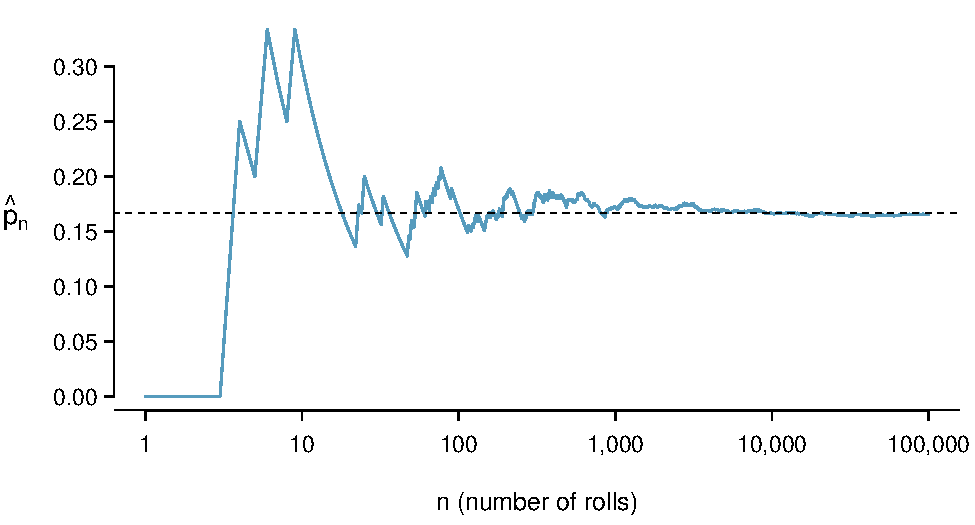
\includegraphics[width=0.8\textwidth]{ch_probability/figures/dieProp/dieProp}
\caption{The fraction of die rolls that are 1 at each stage in a simulation. The relative frequency tends to get closer to the probability $1/6 \approx 0.167$ as the number of rolls increases.}
\label{dieProp}
\end{figure}

\begin{onebox}{Law of Large Numbers}
As more observations are collected, the observed proportion $\hat{p}_n$ of occurrences with a particular outcome after $n$ trials converges to the true probability $p$ of that outcome.\end{onebox}

Occasionally the proportion will veer off from the probability and appear to defy the Law of Large Numbers, as $\hat{p}_n$ does many times in Figure~\ref{dieProp}. However, these deviations become smaller as the number of rolls increases.

Above we write $p$ as the probability of rolling a \resp{1}. We can also write this probability as
\begin{eqnarray*}
P(\text{rolling a \resp{1}})
\end{eqnarray*}

As we become more comfortable with this notation, we will abbreviate it further. For instance, if it is clear that the process is ``rolling a die'', we could abbreviate $P($rolling a \resp{1}$)$ as~$P($\resp{1}$)$.

\begin{exercisewrap}
\begin{nexercise} \label{randomProcessExercise}
Random processes include rolling a die and flipping a coin. (a) Think of another random process. (b) Describe all the possible outcomes of that process. For instance, rolling a die is a random process with potential outcomes \resp{1}, \resp{2}, ...,~\resp{6}.~\footnotemark
\end{nexercise}
\end{exercisewrap}
\footnotetext{Here are four examples. (i) Whether someone gets sick in the next month or not is an apparently random process with outcomes \resp{sick} and \resp{not}. (ii) We can \emph{generate} a random process by randomly picking a person and measuring that person's height. The outcome of this process will be a positive number. (iii) Whether the stock market goes up or down next week is a seemingly random process with possible outcomes \resp{up}, \resp{down}, and \resp{no\us{}change}. Alternatively, we could have used the percent change in the stock market as a numerical outcome. (iv) Whether your roommate cleans her dishes tonight probably seems like a random process with possible outcomes \resp{cleans\us{}dishes} and \resp{leaves\us{}dishes}.}

What we think of as random processes are not necessarily random, but they may just be too difficult to understand exactly. The fourth example in the footnote solution to Guided Practice~\ref{randomProcessExercise} suggests a roommate's behavior is a random process. However, even if a roommate's behavior is not truly random, modeling her behavior as a random process can still be useful.

\begin{onebox}{Modeling a process as random}
It can be helpful to model a process as random even if it is not truly random.\end{onebox}

\index{random process|)}

%%
\subsection{Disjoint or mutually exclusive outcomes}

\index{disjoint|(}
\index{mutually exclusive|(}

Two outcomes are called \term{disjoint} or \term{mutually exclusive} if they cannot both happen in the same trial. For instance, if we roll a die, the outcomes \resp{1} and \resp{2} are disjoint since they cannot both occur on a single roll. On the other hand, the outcomes \resp{1} and ``rolling an odd number'' are not disjoint since both occur if the outcome of the roll is a \resp{1}. The terms \emph{disjoint} and \emph{mutually exclusive} are equivalent and interchangeable.

Calculating the probability of disjoint outcomes is easy. When rolling a die, the outcomes \resp{1} and \resp{2} are disjoint, and we compute the probability that one of these outcomes will occur by adding their separate probabilities:
\begin{eqnarray*}
P(\text{\resp{1} or \resp{2}}) = P(\text{\resp{1}})+P(\text{\resp{2}}) = 1/6 + 1/6 = 1/3
\end{eqnarray*}
What about  the probability of rolling a \resp{1}, \resp{2}, \resp{3}, \resp{4}, \resp{5}, or \resp{6}? Here again, all of the outcomes are disjoint so we add the probabilities:
\begin{eqnarray*}
&&P(\text{\resp{1} or \resp{2} or \resp{3} or \resp{4} or \resp{5} or \resp{6}}) \\
	&&\quad= P(\text{\resp{1}})+P(\text{\resp{2}})+P(\text{\resp{3}})+P(\text{\resp{4}})+P(\text{\resp{5}})+P(\text{\resp{6}}) \\
	&&\quad= 1/6 + 1/6 + 1/6 + 1/6 + 1/6 + 1/6 = 1.
\end{eqnarray*}
The \term{Addition Rule} guarantees the accuracy of this approach when the outcomes are disjoint.

\begin{onebox}{Addition Rule of disjoint outcomes} If $A_1$ and $A_2$ represent two disjoint outcomes, then the probability that one of them occurs is given by
\begin{eqnarray*}
P(A_1\text{ or } A_2) = P(A_1) + P(A_2)
\end{eqnarray*}
If there are many disjoint outcomes $A_1$, ..., $A_k$, then the probability that one of these outcomes will occur is
\begin{eqnarray}
P(A_1) + P(A_2) + \cdots + P(A_k)
\end{eqnarray}
\end{onebox}

\begin{exercisewrap}
\begin{nexercise}
We are interested in the probability of rolling a \resp{1}, \resp{4}, or \resp{5}. (a) Explain why the outcomes \resp{1}, \resp{4}, and \resp{5} are disjoint. (b) Apply the Addition Rule for disjoint outcomes to determine $P($\resp{1} or \resp{4} or \resp{5}$)$.\footnotemark
\end{nexercise}
\end{exercisewrap}
\footnotetext{(a) The random process is a die roll, and at most one of these outcomes can come up. This means they are disjoint outcomes. (b)~$P($\resp{1} or \resp{4} or \resp{5}$) = P($\resp{1}$)+P($\resp{4}$)+P($\resp{5}$) = \frac{1}{6} + \frac{1}{6} + \frac{1}{6} = \frac{3}{6} = \frac{1}{2}$}

\index{data!email|(}
\begin{exercisewrap}
\begin{nexercise}
In the \data{email} data set in Chapter~\ref{summarizingData}, the \var{number} variable described whether no number (labeled \resp{none}), only one or more small numbers (\resp{small}), or whether at least one big number appeared in an email (\resp{big}). Of the 3,921 emails, 549 had no numbers, 2,827 had only one or more small numbers, and 545 had at least one big number. (a) Are the outcomes \resp{none}, \resp{small}, and \resp{big} disjoint? (b) Determine the proportion of emails with value \resp{small} and \resp{big} separately. (c) Use the Addition Rule for disjoint outcomes to compute the probability a randomly selected email from the data set has a number in it, small or big.\footnotemark
\end{nexercise}
\end{exercisewrap}
\footnotetext{(a) Yes. Each email is categorized in only one level of \var{number}. (b) Small: $\frac{2827}{3921} = 0.721$. Big: $\frac{545}{3921} = 0.139$. (c) $P($\resp{small} or \resp{big}$) = P($\resp{small}$) + P($\resp{big}$) = 0.721 + 0.139 = 0.860$.}
\index{data!email|)}

\index{event|(}

Statisticians rarely work with individual outcomes and instead consider \indexthis{\emph{sets}}{sets} or \indexthis{\emph{collections}}{collections} of outcomes. Let $A$ represent the event where a die roll results in \resp{1} or \resp{2} and $B$~represent the event that the die roll is a \resp{4} or a \resp{6}. We write $A$ as the set of outcomes $\{$\resp{1},~\resp{2}$\}$ and $B=\{$\resp{4}, \resp{6}$\}$. These sets are commonly called \termsub{events}{event}. Because $A$ and $B$ have no elements in common, they are disjoint events. $A$ and $B$ are represented in Figure~\ref{disjointSets}.

\begin{figure}[hhh]
\centering
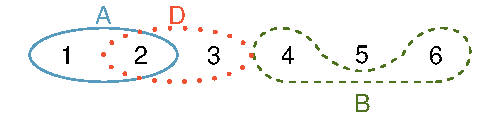
\includegraphics[height=0.7in]{ch_probability/figures/disjointSets/disjointSets}
\caption{Three events, $A$, $B$, and $D$, consist of outcomes from rolling a die. $A$ and $B$ are disjoint since they do not have any outcomes in common.}
\label{disjointSets}
\end{figure}

\D{\newpage}

The Addition Rule applies to both disjoint outcomes and disjoint events. The probability that one of the disjoint events $A$ or $B$ occurs is the sum of the separate probabilities:
\begin{eqnarray*}
P(A\text{ or }B) = P(A) + P(B) = 1/3 + 1/3 = 2/3
\end{eqnarray*}

\begin{exercisewrap}
\begin{nexercise}
(a) Verify the probability of event $A$, $P(A)$, is $1/3$ using the Addition Rule. (b) Do the same for event $B$.\footnotemark
\end{nexercise}
\end{exercisewrap}
\footnotetext{(a) $P(A) = P($\resp{1} or \resp{2}$) = P($\resp{1}$) + P($\resp{2}$) = \frac{1}{6} + \frac{1}{6} = \frac{2}{6} = \frac{1}{3}$. (b) Similarly, $P(B) = 1/3$.}

\begin{exercisewrap}
\begin{nexercise} \label{exerExaminingDisjointSetsABD}
(a) Using Figure~\ref{disjointSets} as a reference, what outcomes are represented by event $D$? (b) Are events $B$ and $D$ disjoint? (c) Are events $A$ and $D$ disjoint?\footnotemark
\end{nexercise}
\end{exercisewrap}
\footnotetext{(a)~Outcomes \resp{2} and \resp{3}. (b)~Yes, events $B$ and $D$ are disjoint because they share no outcomes. (c)~The events $A$ and $D$ share an outcome in common, \resp{2}, and so are not disjoint.}

\begin{exercisewrap}
\begin{nexercise}
In Guided Practice~\ref{exerExaminingDisjointSetsABD}, you confirmed $B$ and $D$ from Figure~\ref{disjointSets} are disjoint. Compute the probability that either event $B$ or event $D$ occurs.\footnotemark
\end{nexercise}
\end{exercisewrap}
\footnotetext{Since $B$ and $D$ are disjoint events, use the Addition Rule: $P(B$ or $D) = P(B) + P(D) = \frac{1}{3} + \frac{1}{3} = \frac{2}{3}$.}

\index{event|)}
\index{disjoint|)}
\index{mutually exclusive|)}

%%
\subsection{Probabilities when events are not disjoint}

Let's consider calculations for two events that are not disjoint in the context of a \indexthis{regular deck of 52 cards}{deck of cards}, represented in Figure~\ref{deckOfCards}. If you are unfamiliar with the cards in a regular deck, please see the footnote.\footnote{The 52 cards are split into four \term{suits}: $\clubsuit$ (club), {\color{redcards}$\diamondsuit$} (diamond), {\color{redcards}$\heartsuit$} (heart), $\spadesuit$ (spade). Each suit has its 13 cards labeled: \resp{2}, \resp{3}, ..., \resp{10}, \resp{J} (jack), \resp{Q} (queen), \resp{K} (king), and \resp{A} (ace). Thus, each card is a unique combination of a suit and a label, e.g. {\color{redcards}\resp{4$\heartsuit$}} and \resp{J$\clubsuit$}. The 12 cards represented by the jacks, queens, and kings are called \termsub{\resp{face cards}}{face card}. The cards that are {\color{redcards}$\diamondsuit$} or {\color{redcards}$\heartsuit$} are typically colored {\color{redcards}red} while the other two suits are typically colored black.}

\begin{figure}[h]
\centering
\begin{tabular}{lll lll lll lll l}
\resp{2$\clubsuit$} & \resp{3$\clubsuit$} & \resp{4$\clubsuit$} & \resp{5$\clubsuit$} & \resp{6$\clubsuit$} & \resp{7$\clubsuit$} & \resp{8$\clubsuit$} & \resp{9$\clubsuit$} & \resp{10$\clubsuit$} & \resp{J$\clubsuit$} & \resp{Q$\clubsuit$} & \resp{K$\clubsuit$} & \resp{A$\clubsuit$}  \\
\color{redcards} \resp{2$\diamondsuit$} & \color{redcards}\resp{3$\diamondsuit$} & \color{redcards}\resp{4$\diamondsuit$} & \color{redcards}\resp{5$\diamondsuit$} & \color{redcards}\resp{6$\diamondsuit$} & \color{redcards}\resp{7$\diamondsuit$} & \color{redcards}\resp{8$\diamondsuit$} & \color{redcards}\resp{9$\diamondsuit$} & \color{redcards}\resp{10$\diamondsuit$} & \color{redcards}\resp{J$\diamondsuit$} & \color{redcards}\resp{Q$\diamondsuit$} & \color{redcards}\resp{K$\diamondsuit$} & \color{redcards}\resp{A$\diamondsuit$} \\
\color{redcards}\resp{2$\heartsuit$} & \color{redcards}\resp{3$\heartsuit$} & \color{redcards}\resp{4$\heartsuit$} & \color{redcards}\resp{5$\heartsuit$} & \color{redcards}\resp{6$\heartsuit$} & \color{redcards}\resp{7$\heartsuit$} & \color{redcards}\resp{8$\heartsuit$} & \color{redcards}\resp{9$\heartsuit$} & \color{redcards}\resp{10$\heartsuit$} & \color{redcards}\resp{J$\heartsuit$} & \color{redcards}\resp{Q$\heartsuit$} & \color{redcards}\resp{K$\heartsuit$} & \color{redcards}\resp{A$\heartsuit$} \\
\resp{2$\spadesuit$} & \resp{3$\spadesuit$} & \resp{4$\spadesuit$} & \resp{5$\spadesuit$} & \resp{6$\spadesuit$} & \resp{7$\spadesuit$} & \resp{8$\spadesuit$} & \resp{9$\spadesuit$} & \resp{10$\spadesuit$} & \resp{J$\spadesuit$} & \resp{Q$\spadesuit$} & \resp{K$\spadesuit$} & \resp{A$\spadesuit$}
\end{tabular}
\caption{Representations of the 52 unique cards in a deck.}
\label{deckOfCards}
\end{figure}

\begin{exercisewrap}
\begin{nexercise}
(a) What is the probability that a randomly selected card is a diamond? (b)~What is the probability that a randomly selected card is a face~card?\footnotemark
\end{nexercise}
\end{exercisewrap}
\footnotetext{(a) There are 52 cards and 13 diamonds. If the cards are thoroughly shuffled, each card has an equal chance of being drawn, so the probability that a randomly selected card is a diamond is $P({\color{redcards}\diamondsuit}) = \frac{13}{52} = 0.250$. (b)~Likewise, there are 12 face cards, so $P($face card$) = \frac{12}{52} = \frac{3}{13} = 0.231$.}

\term{Venn diagrams} are useful when outcomes can be categorized as ``in'' or ``out'' for two or three variables, attributes, or random processes. The Venn diagram in Figure~\ref{venn} uses a circle to represent diamonds and another to represent face cards. If a card is both a diamond and a face card, it falls into the intersection of the circles. If it is a diamond but not a face card, it will be in part of the left circle that is not in the right circle (and so on). The total number of cards that are diamonds is given by the total number of cards in the diamonds circle: $10+3=13$. The probabilities are also shown (e.g. $10/52 = 0.1923$).

\begin{figure}
\centering
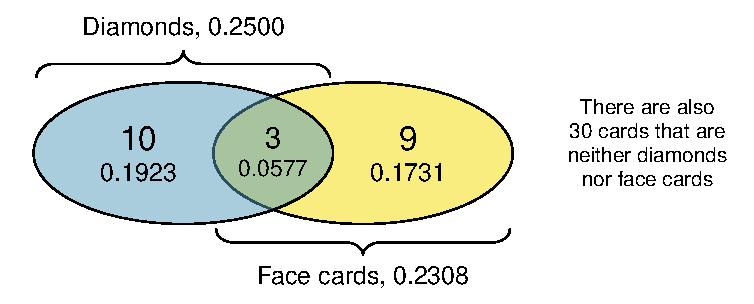
\includegraphics[height=1.4in]{ch_probability/figures/venn/venn}
\caption{A Venn diagram for diamonds and face cards.}
\label{venn}
\end{figure}

\begin{exercisewrap}
\begin{nexercise}
Using the Venn diagram, verify $P($face card$) = 12/52=3/13$.\footnotemark\end{nexercise}
\end{exercisewrap}
\footnotetext{The Venn diagram shows face cards split up into ``face card but not {\color{redcards}$\diamondsuit$}'' and ``face card and {\color{redcards}$\diamondsuit$}''. Since these correspond to disjoint events, $P($face card$)$ is found by adding the two corresponding probabilities: $\frac{3}{52} + \frac{9}{52} = \frac{12}{52} = \frac{3}{13}$.}


Let $A$ represent the event that a randomly selected card is a diamond and $B$ represent the event that it is a face card. How do we compute $P(A$ or $B)$? Events $A$ and $B$ are not disjoint -- the cards {\color{redcards}$J\diamondsuit$}, {\color{redcards}$Q\diamondsuit$}, and {\color{redcards}$K\diamondsuit$} fall into both categories -- so we cannot use the Addition Rule for disjoint events. Instead we use the Venn diagram. We start by adding the probabilities of the two events:
\begin{eqnarray*}
P(A) + P(B) = P({\color{redcards}\diamondsuit}) + P(\text{face card}) = 13/52 + 12/52
\label{overCountFaceDiamond}
\end{eqnarray*}
However, the three cards that are in both events were counted twice, once in each probability. We must correct this double counting:
\begin{eqnarray}
P(A\text{ or } B) &=&P({\color{redcards}\diamondsuit}) + P(\text{face card})  \notag \\
 &=& P({\color{redcards}\diamondsuit}) + P(\text{face card}) - P({\color{redcards}\diamondsuit}  \text{ and face card}) \label{diamondFace} \\
 &=& 13/52 + 12/52 - 3/52 \notag \\
 &=& 22/52 = 11/26 \notag
\end{eqnarray}
Equation~(\ref{diamondFace}) is an example of the \term{General Addition Rule}.

\begin{onebox}{General Addition Rule}
If $A$ and $B$ are any two events, disjoint or not, then the probability that A or B will occur is
\begin{eqnarray}
P(A\text{ or }B) = P(A) + P(B) - P(A\text{ and }B)
\label{generalAdditionRule}
\end{eqnarray}
where $P(A$ and $B)$ is the probability that both events occur.\end{onebox}


\begin{onebox}{Symbolic notation for ``and" and ``or"}
The symbol $\cap$ means intersection and is equivalent to ``and".

The symbol  $\cup$ means union and is equivalent to ``or".

It is common to see the General Addition Rule written as
\begin{eqnarray}
P(A \cup B) = P(A) + P(B) - P(A \cap B)
\end{eqnarray}
\end{onebox}

\begin{onebox}{``or'' is inclusive}
When we write, ``or"  in statistics, we mean ``and/or'' unless we explicitly state otherwise. Thus, $A$ or $B$ occurs means $A$, $B$, or both $A$ and $B$ occur. This is equivalent to at least one of $A$ or $B$ occurring.\end{onebox}

\begin{exercisewrap}
\begin{nexercise}
(a) If $A$ and $B$ are disjoint, describe why this implies $P(A$ and $B) = 0$. (b) Using part (a), verify that the General Addition Rule simplifies to the simpler Addition Rule for disjoint events if $A$ and $B$ are disjoint.\footnotemark
\end{nexercise}
\end{exercisewrap}
\footnotetext{(a) If $A$ and $B$ are disjoint, $A$ and $B$ can never occur simultaneously. (b) If $A$ and $B$ are disjoint, then the last term of Equation~(\ref{generalAdditionRule}) is 0 (see part (a)) and we are left with the Addition Rule for disjoint events.}

\index{data!email|(}

\begin{exercisewrap}
\begin{nexercise}\label{emailSpamNumberVennExer}
% library(openintro); data(email); table(email[,c("spam", "number")]); table(email[,c("number")]); table(email[,c("spam")])
In the \data{email} data set with 3,921 emails, 367 were spam, 2,827 contained some small numbers but no big numbers, and 168 had both characteristics. Create a Venn diagram for this setup.\footnotemark
\end{nexercise}
\end{exercisewrap}
\footnotetext{%
\begin{minipage}[t]{0.65\textwidth}
Both the counts and corresponding {\color{oiB}probabilities} (e.g. $2659/3921 = 0.678$) are shown. Notice that the number of emails represented in the left circle corresponds to $2659 + 168 = 2827$, and the number represented in the right circle is $168 + 199 = 367$.
\end{minipage}\ %
\begin{minipage}[c]{0.3\textwidth}
\hfill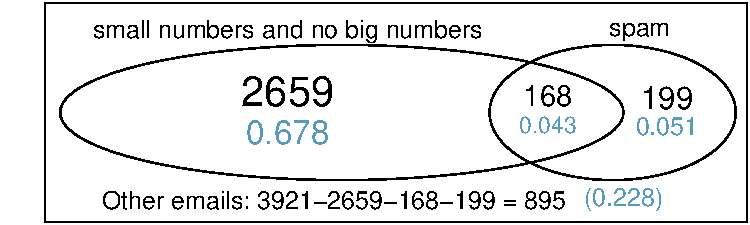
\includegraphics[height=13mm]{ch_probability/figures/emailSpamNumberVenn/emailSpamNumberVenn} \vspace{-13mm}
\end{minipage}
}

\begin{exercisewrap}
\begin{nexercise}
(a) Use your Venn diagram from Guided Practice~\ref{emailSpamNumberVennExer} to determine the probability a randomly drawn email from the \data{email} data set is spam and had small numbers (but not big numbers). (b)~What is the probability that the email had either of these attributes?\footnotemark
\index{data!email|)}
\end{nexercise}
\end{exercisewrap}
\footnotetext{(a)~The solution is represented by the intersection of the two circles: 0.043. (b)~This is the sum of the three disjoint probabilities shown in the circles: $0.678 + 0.043 + 0.051 = 0.772$.}


%%
\subsection{Complement of an event}

Rolling a die produces a value in the set $\{$\resp{1}, \resp{2}, \resp{3}, \resp{4}, \resp{5}, \resp{6}$\}$. This set of all possible outcomes is called the \term{sample space} ($S$) for rolling a die. We often use the sample space to examine the scenario where an event does not occur.

Let $D=\{$\resp{2}, \resp{3}$\}$ represent the event that the outcome of a die roll is \resp{2} or \resp{3}. Then the \term{complement} represents all outcomes in our sample space that are not in $D$, which is denoted by $D^c = \{$\resp{1}, \resp{4}, \resp{5}, \resp{6}$\}$. That is, $D^c$ is the set of all possible outcomes not already included in $D$. Figure~\ref{complementOfD} shows the relationship between $D$, $D^c$, and the sample space $S$.

\begin{figure}[hht]
\centering
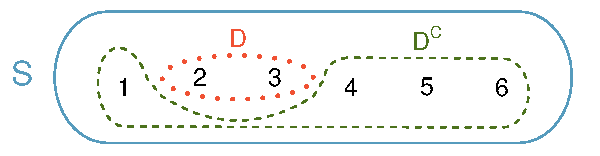
\includegraphics[width=0.5\textwidth]{ch_probability/figures/complementOfD/complementOfD}
\caption{Event $D=\{$\resp{2}, \resp{3}$\}$ and its complement, $D^c = \{$\resp{1}, \resp{4}, \resp{5}, \resp{6}$\}$. $S$~represents the sample space, which is the set of all possible events.}
\label{complementOfD}

\end{figure}

\begin{exercisewrap}
\begin{nexercise}
(a) Compute $P(D^c) = P($rolling a \resp{1}, \resp{4}, \resp{5}, or \resp{6}$)$. (b) What is $P(D) + P(D^c)$?\footnotemark
\end{nexercise}
\end{exercisewrap}
\footnotetext{(a)~The outcomes are disjoint and each has probability $1/6$, so the total probability is $4/6=2/3$. (b)~We can also see that $P(D)=\frac{1}{6} + \frac{1}{6} = 1/3$. Since $D$ and $D^c$ are disjoint, $P(D) + P(D^c) = 1$.}

\D{\newpage}

\begin{exercisewrap}
\begin{nexercise}
Events $A=\{$\resp{1}, \resp{2}$\}$ and $B=\{$\resp{4}, \resp{6}$\}$ are shown in Figure~\ref{disjointSets} on page~\pageref{disjointSets}. (a) Write out what $A^c$ and $B^c$ represent. (b)~Compute $P(A^c)$ and $P(B^c)$. (c)~Compute $P(A)+P(A^c)$ and $P(B)+P(B^c)$.\footnotemark\end{nexercise}
\end{exercisewrap}
\footnotetext{Brief solutions: (a)~$A^c=\{$\resp{3}, \resp{4}, \resp{5}, \resp{6}$\}$ and $B^c=\{$\resp{1}, \resp{2}, \resp{3}, \resp{5}$\}$. (b)~Noting that each outcome is disjoint, add the individual outcome probabilities to get $P(A^c)=2/3$ and $P(B^c)=2/3$. (c)~$A$~and~$A^c$ are disjoint, and the same is true of $B$~and~$B^c$. Therefore, $P(A) + P(A^c) = 1$ and $P(B) + P(B^c) = 1$.}


An event $A$ together with its complement $A^c$ comprise the entire sample space. Because of this we can say that $P(A) + P(A^c) = 1$.

\begin{onebox}{Complement}
The complement of event $A$ is denoted $A^c$, and $A^c$ represents all outcomes not in~$A$. $A$ and $A^c$ are mathematically related: \vspace{-2mm}
\begin{eqnarray}\label{complement}
P(A) + P(A^c) = 1, \quad\text{i.e.}\quad P(A) = 1-P(A^c)
\end{eqnarray}\vspace{-6.5mm}\end{onebox}

In simple examples, computing $A$ or $A^c$ is feasible in a few steps. However, using the complement can save a lot of time as problems grow in complexity.

\begin{exercisewrap}
\begin{nexercise}
A die is rolled 10 times. (a)~What is the complement of getting at least one 6 in 10 rolls of the die? (b)~What is the complement of getting at most three 6's in 10 rolls of the die?\footnotemark
\end{nexercise}
\end{exercisewrap}
\footnotetext{(a)~The complement of getting at least one 6 in ten rolls of a die is getting zero 6's in the 10 rolls. (b)~The complement of getting at most three 6's in 10 rolls is getting four, five, ..., nine, or ten 6's in 10~rolls.}


%%
\subsection{Independence}
\label{probabilityIndependence}

Just as variables and observations can be independent, random processes can be independent, too. Two processes are \term{independent} if knowing the outcome of one provides no useful information about the outcome of the other. For instance, flipping a coin and rolling a die are two independent processes -- knowing the coin was heads does not help determine the outcome of a die roll. On the other hand, stock prices usually move up or down together, so they are not independent.

Example~\ref{probOf2Ones} provides a basic example of two independent processes: rolling two dice. We want to determine the probability that both will be \resp{1}. Suppose one of the dice is red and the other white. If the outcome of the red die is a \resp{1}, it provides no information about the outcome of the white die. We first encountered this same question in Example~\ref{probOf2Ones} (page~\pageref{probOf2Ones}), where we calculated the probability using the following reasoning: $1/6^{th}$ of the time the red die is a \resp{1}, and $1/6^{th}$ of \emph{those} times the white die will also be \resp{1}. This is illustrated in Figure~\ref{indepForRollingTwo1s}. Because the rolls are independent, the probabilities of the corresponding outcomes can be multiplied to get the final answer: $(1/6)\times(1/6)=1/36$. This can be generalized to many independent processes.

\begin{figure}[hht]
\centering
\Figure{0.55}{indepForRollingTwo1s}
\caption{$1/6^{th}$ of the time, the first roll is a \resp{1}. Then $1/6^{th}$ of \emph{those} times, the second roll will also be a \resp{1}.}
\label{indepForRollingTwo1s}
\end{figure}

\begin{examplewrap}
\begin{nexample}{What if there was also a blue die independent of the other two? What is the probability of rolling the three dice and getting all \resp{1}s?}\label{threeDice}
The same logic applies from Example~\ref{probOf2Ones}. If $1/36^{th}$ of the time the white and red dice are both \resp{1}, then $1/6^{th}$ of \emph{those} times the blue die will also be \resp{1}, so multiply:
{\begin{align*}
P(white=\text{\small\resp{1} and } red=\text{\small\resp{1} and } blue=\text{\small\resp{1}})
	&= P(white=\text{\small\resp{1}})\times P(red=\text{\small\resp{1}})\times P(blue=\text{\small\resp{1}}) \\
	&= (1/6)\times (1/6)\times (1/6)
	= 1/216
\end{align*}} \vspace{-7mm}
\end{nexample}
\end{examplewrap}

Examples~\ref{probOf2Ones} and~\ref{threeDice} illustrate what is called the Multiplication Rule for independent processes.

\begin{onebox}{Multiplication Rule for independent processes}\index{Multiplication Rule}
If $A$ and $B$ represent events from two different and independent processes, then the probability that both $A$ and $B$ occur can be calculated as the product of their separate probabilities: \vspace{-1.5mm}
\begin{eqnarray}\label{eqForIndependentEvents}
P(A \text{ and }B) = P(A) \times  P(B)
\end{eqnarray}
Similarly, if there are $k$ events $A_1$, ..., $A_k$ from $k$ independent processes, then the probability they all occur is\vspace{-1.5mm}
\begin{eqnarray*}
P(A_1) \times  P(A_2)\times  \cdots \times  P(A_k)
\end{eqnarray*}\vspace{-6mm}\end{onebox}

\begin{exercisewrap}
\begin{nexercise} \label{ex2Handedness}
About 9\% of people are left-handed. Suppose 2 people are selected at random from the U.S. population. Because the sample size of 2 is very small relative to the population, it is reasonable to assume these two people are independent. (a)~What is the probability that both are left-handed? (b)~What is the probability that both are right-handed?\footnotemark
\end{nexercise}
\end{exercisewrap}
\footnotetext{(a) The probability the first person is left-handed is $0.09$, which is the same for the second person. We apply the Multiplication Rule for independent processes to determine the probability that both will be left-handed: $0.09\times 0.09 = 0.0081$.

(b) It is reasonable to assume the proportion of people who are ambidextrous (both right- and left-handed) is nearly 0, which results in $P($right-handed$)=1-0.09=0.91$. Using the same reasoning as in part~(a), the probability that both will be right-handed is $0.91\times 0.91 = 0.8281$.}

\begin{exercisewrap}
\begin{nexercise} \label{ex5Handedness}
Suppose 5 people are selected at random.\footnotemark{}\vspace{-1.5mm}
\begin{enumerate}
\setlength{\itemsep}{0mm}
\item[(a)] What is the probability that all are right-handed?
\item[(b)] What is the probability that all are left-handed?
\item[(c)] What is the probability that not all of the people are right-handed?
\end{enumerate}
\end{nexercise}
\end{exercisewrap}
\footnotetext{(a)~The abbreviations \resp{RH} and \resp{LH} are used for right-handed and left-handed, respectively. Since each are independent, we apply the Multiplication Rule for independent processes:
\begin{align*}
P(\text{all five are \resp{RH}})
&= P(\text{first = \resp{RH}, second = \resp{RH}, ..., fifth = \resp{RH}}) \\
&= P(\text{first = \resp{RH}})\times P(\text{second = \resp{RH}})\times  \dots \times P(\text{fifth = \resp{RH}}) \\
&= 0.91\times 0.91\times 0.91\times 0.91\times 0.91 = 0.624
\end{align*}

(b)~Using the same reasoning as in~(a), $0.09\times 0.09\times 0.09\times 0.09\times 0.09 = 0.0000059$

(c)~Use the complement, $P($all five are \resp{RH}$)$, to answer this question:
\begin{align*}
P(\text{not all \resp{RH}})
	= 1 - P(\text{all \resp{RH}})
	= 1 - 0.624 = 0.376
\end{align*}} 

\D{\newpage}

Suppose the variables \var{handedness} and \var{gender} are independent, i.e. knowing someone's \var{gender} provides no useful information about their \var{handedness} and vice-versa. Then we can compute whether a randomly selected person is right-handed and female\footnote{The actual proportion of the U.S. population that is \resp{female} is about 50\%, and so we use 0.5 for the probability of sampling a woman. However, this probability does differ in other countries.} using the Multiplication Rule:
\begin{eqnarray*}
P(\text{right-handed and female}) &=& P(\text{right-handed}) \times  P(\text{female}) \\
&=& 0.91 \times  0.50 = 0.455
\end{eqnarray*}


\begin{exercisewrap}
\begin{nexercise}
Three people are selected at random.\footnotemark \vspace{-1.5mm}
\begin{enumerate}
\setlength{\itemsep}{0mm}
\item[(a)] What is the probability that the first person is male and right-handed?
\item[(b)] What is the probability that the first two people are male and right-handed?.
\item[(c)] What is the probability that the third person is female and left-handed?
\item[(d)] What is the probability that the first two people are male and right-handed and the third person is female and left-handed?
\end{enumerate}
\end{nexercise}
\end{exercisewrap}
\footnotetext{Brief answers are provided. (a)~This can be written in probability notation as $P($a randomly selected person is male and right-handed$)=0.455$. (b) 0.207. (c) 0.045. (d) 0.0093.}

Sometimes we wonder if one outcome provides useful information about another outcome. The question we are asking is, are the occurrences of the two events independent? We say that two events $A$ and $B$ are independent if they satisfy Equation~\eqref{eqForIndependentEvents}.

\begin{examplewrap}
\begin{nexample}{If we shuffle up a deck of cards and draw one, is the event that the card is a heart independent of the event that the card is an ace?}
The probability the card is a heart is $1/4$ and the probability that it is an ace is $1/13$. The probability the card is the ace of hearts is $1/52$. We check whether Equation~\ref{eqForIndependentEvents} is satisfied:
\begin{align*}
P({\color{redcards}\heartsuit})\times P(\text{ace}) = \frac{1}{4}\times \frac{1}{13} = \frac{1}{52}
					= P({\color{redcards}\heartsuit}\text{ and ace})
\end{align*}
Because the equation holds, the event that the card is a heart and the event that the card is an ace are independent events.
\end{nexample}
\end{examplewrap}


\D{\newpage}

%%
\subsection*{Section summary}

\begin{itemize}

\item When an outcome depends upon a chance process, we can define the \term{probability} of the outcome as the proportion of times it would occur if we repeated the process an infinite number of times.  Also, even when an outcome is not truly random, modeling it with probability can be useful.

\item The \term{Law of Large Numbers} states that the \term{relative frequency}, or proportion of times an outcome occurs after $n$ repetitions, stabilizes around the true probability as $n$ gets large.

\item The probability of an event is always between 0 and 1, inclusive.

\item The probability of an event and the probability of its \term{complement} add up to 1.  Sometime we use $P(A) = 1- P(\text{not } A)$ when $P(\text{not }A)$ is easier to calculate than $P(A)$.

\item $A$ and $B$ are \term{disjoint}, i.e. \term{mutually exclusive}, if they cannot happen together.  In this case, the events do not overlap and $P(A \text { and } B) = 0$.

\item In the \emph{special case} where $A$ and $B$ are \term{disjoint} events:  $P(A \text{ or } B) = P(A) + P(B)$.  

\item When $A$ and $B$ are not disjoint, adding $P(A)$ and $P(B)$ will overestimate $P(A \text{ or } B)$ because the overlap of $A$ and $B$ will be added twice.  Therefore, when $A$ and $B$ are not disjoint, use the \term{General Addition Rule}:  \\$P(A \text{ or  B}) = P(A) + P(B) - P(A \text{ and } B)$.\footnote{Often written: $P(A \cup B) = P(A) + P(B) - P(A \cap B)$.} 

\item To find the probability that \emph{at least one} of several events occurs, use a special case of the rule of \termsub{complements}{rule of complements}\index{complement}:  $P(\text{at least one}) = 1- P(\text{none})$.  

\item When only considering two events, the probability that one \emph{or} the other happens is equal to the probability that \emph{at least one} of the two events happens.  When dealing with more than two events, the General Addition Rule becomes very complicated.  Instead, to find the probability that $A$ or $B$ or $C$ occurs, find the probability that none of them occur and subtract that value from 1.  

\item Two events are \term{independent} when the occurrence of one does not change the likelihood of the other.

\item In the \emph{special case} where $A$ and $B$ are \term{independent}:
$P(A \text{ and } B) = P(A)\times P(B)$.

\end{itemize}

%%%%%%%%%Section Exercises
{\exercisesheader{}

% 1 - tf_prob_definitions

\eoce{\qt{True or false\label{tf_prob_definitions}} Determine if the statements 
below are true or false, and explain your reasoning.
\begin{parts}
\item If a fair coin is tossed many times and the last eight tosses are all heads, 
then the chance that the next toss will be heads is somewhat less than 50\%.
\item Drawing a face card (jack, queen, or king) and drawing a red card from a 
full deck of playing cards are mutually exclusive events.
\item Drawing a face card and drawing an ace from a full deck of playing cards 
are mutually exclusive events.
\end{parts}
}{}

% 2 - roulette_wheel

\eoce{\qt{Roulette wheel\label{roulette_wheel}} The game of roulette involves 
spinning a wheel with 38 slots: 18 red, 18 black, and 2 green. A ball is spun 
onto the wheel and will eventually land in a slot, where each slot has an equal 
chance of capturing the ball.

\noindent%
\begin{minipage}[c]{0.65\textwidth}
\raggedright\begin{parts}
\item You watch a roulette wheel spin 3 consecutive times and the ball lands on a 
red slot each time. What is the probability that the ball will land on a red slot 
on the next spin?
\item You watch a roulette wheel spin 300 consecutive times and the ball lands on 
a red slot each time. What is the probability that the ball will land on a red 
slot on the next spin?
\item Are you equally confident of your answers to parts~(a) and~(b)? Why or why 
not?
\end{parts}
\end{minipage}
\begin{minipage}[c]{0.05\textwidth}
\ 
\end{minipage}
\begin{minipage}[c]{0.28\textwidth}
\begin{center}
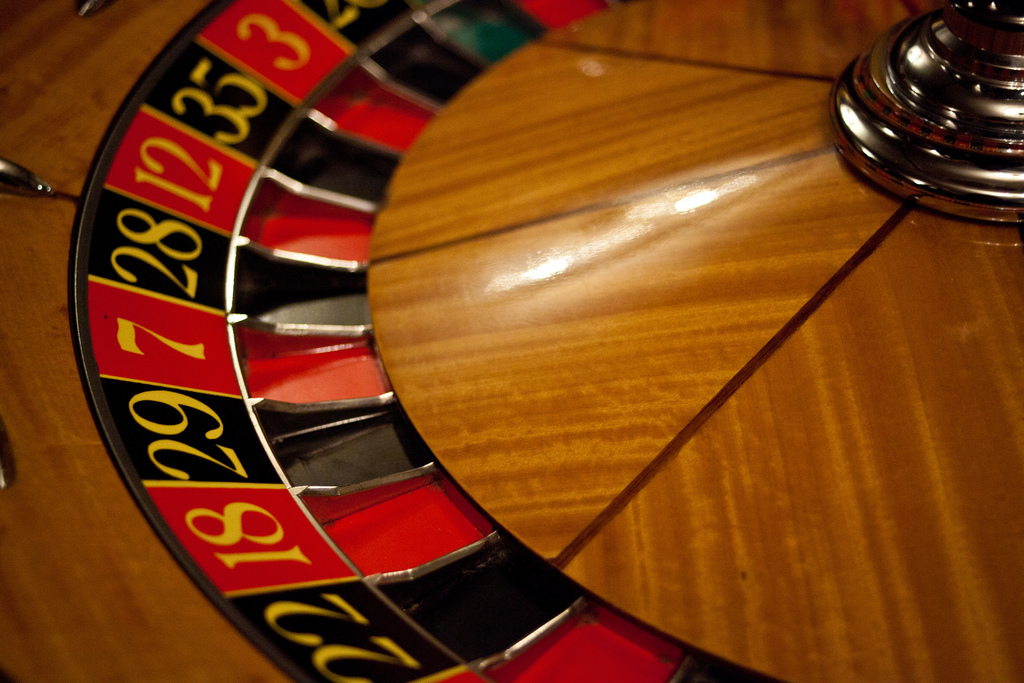
\includegraphics[width = \textwidth]{ch_probability/figures/eoce/roulette_wheel/roulette_wheel.jpg} \\
{\footnotesize Photo by H\r{a}kan Dahlstr\"{o}m \\
  (\oiRedirect{textbook-flickr_hakan_dahlstrom_roulette_wheel}{http://flic.kr/p/93fEzp}) \\
  \oiRedirect{textbook-CC_BY_2}{CC~BY~2.0~license}}
\end{center}
\end{minipage}
}{}

% 3 - four_games_one_winner

\eoce{\qt{Four games, one winner\label{four_games_one_winner}} \videosolution{ahss_eoce_sol-global_warming} Below are four 
versions of the same game. Your archnemesis gets to pick the version of the game, 
and then you get to choose how many times to flip a coin: 10 times or 100 times. 
Identify how many coin flips you should choose for each version of the game. It 
costs \$1 to play each game. Explain your reasoning.
\begin{parts}
\item If the proportion of heads is larger than 0.60, you win \$1.
\item If the proportion of heads is larger than 0.40, you win \$1.
\item If the proportion of heads is between 0.40 and 0.60, you win \$1.
\item If the proportion of heads is smaller than 0.30, you win \$1.
\end{parts}
}{}

% 4 - backgammon

\eoce{\qt{Backgammon\label{backgammon}} Backgammon is a board game for two 
players in which the playing pieces are moved according to the roll of two dice. 
Players win by removing all of their pieces from the board, so it is usually good 
to roll high numbers. You are playing backgammon with a friend and you roll two 
6s in your first roll and two 6s in your second roll. Your friend rolls two 3s in 
his first roll and again in his second row. Your friend claims that you are 
cheating, because rolling double 6s twice in a row is very unlikely. Using 
probability, show that your rolls were just as likely as~his.
}{}

% 5 - coin_flips

\eoce{\qt{Coin flips\label{coin_flips}} If you flip a fair coin 10 times, what is 
the probability of
\begin{parts}
\item getting all tails? 
\item getting all heads? 
\item getting at least one tails? 
\end{parts}
}{}

% 6 - dice_rolls

\eoce{\qt{Dice rolls\label{dice_rolls}} If you roll a pair of fair dice, what is 
the probability of
\begin{parts}
\item getting a sum of 1?
\item getting a sum of 5?
\item getting a sum of 12?
\end{parts}
}{}

\D{\newpage}

% 7 - swing_voters

\eoce{\qt{Swing voters\label{swing_voters}} \videosolution{ahss_eoce_sol-global_warming}  A Pew Research survey asked 2,373 
randomly sampled registered voters their political affiliation (Republican, 
Democrat, or Independent) and whether or not they identify as swing voters. 35\% 
of respondents identified as Independent, 23\% identified as swing voters, and 
11\% identified as both.\footfullcite{indepSwing}
\begin{parts}
\item Are being Independent and being a swing voter disjoint, i.e. mutually 
exclusive?
\item Draw a Venn diagram summarizing the variables and their associated 
probabilities.
\item What percent of voters are Independent but not swing voters?
\item What percent of voters are Independent or swing voters?
\item What percent of voters are neither Independent nor swing voters?
\item Is the event that someone is a swing voter independent of the event that 
someone is a political Independent?
\end{parts}
}{}

% 8 - poverty_language

\eoce{\qt{Poverty and language\label{poverty_language}} The American Community 
Survey is an ongoing survey that provides data every year to give communities the 
current information they need to plan investments and services. The 2010 American 
Community Survey estimates that 14.6\% of Americans live below the poverty line, 
20.7\% speak a language other than English (foreign language) at home, and 4.2\% 
fall into both categories. \footfullcite{poorLang}
\begin{parts}
\item Are living below the poverty line and speaking a foreign language at home 
disjoint?
\item Draw a Venn diagram summarizing the variables and their associated 
probabilities.
\item What percent of Americans live below the poverty line and only speak 
English at home?
\item What percent of Americans live below the poverty line or speak a foreign 
language at home?
\item What percent of Americans live above the poverty line and only speak 
English at home? 
\item Is the event that someone lives below the poverty line independent of the 
event that the person speaks a foreign language at home?
\end{parts}
}{}

% 9 - disjoint_indep

\eoce{\qt{Disjoint vs. independent\label{disjoint_indep}} In parts~(a) and~(b), 
identify whether the events are disjoint, independent, or neither (events cannot 
be both disjoint and independent).
\begin{parts}
\item You and a randomly selected student from your class both earn A's in this 
course. 
\item You and your class study partner both earn A's in this course.
\item If two events can occur at the same time, must they be dependent?
\end{parts}
}{}

% 10 - guessing_on_exam

\eoce{\qt{Guessing on an exam\label{guessing_on_exam}} In a multiple choice exam, 
there are 5 questions and 4 choices for each question (a, b, c, d). Nancy has not 
studied for the exam at all and decides to randomly guess the answers. What is 
the probability that:
\begin{parts}
\item the first question she gets right is the $5^{th}$ question?
\item she gets all of the questions right?
\item she gets at least one question right?
\end{parts}
}{}

\D{\newpage}

% 11 - edu_attain_parent_teen

\eoce{\qt{Educational attainment\label{edu_attain_parent_teen}} The \data{family\_\hspace{0.3mm}college} data set contains a sample of 792 cases with two variables, \var{teen} and \var{parents}, and is summarized below.\footnote{A simulated data set based on real population summaries at \oiRedirect{textbook-student_parent_college_2001}{nces.ed.gov/pubs2001/2001126.pdf}.} The \var{teen} variable is either \resp{college} or \resp{not}, where the \var{college} label means the teen went to college immediately after high school. The~\var{parents} variable takes the value \resp{degree} if at least one parent of the teenager completed a college degree.

\begin{table}[ht]
\centering
\begin{tabular}{ll rr r rr}
  && \multicolumn{2}{c}{\var{parents}} & \hspace{1cm} &  \\
  \cline{3-4}
	&& \resp{degree} & \resp{not} & Total  \\
  \cline{2-5}
	& \resp{college}     & 231 & 214 & 445 \\
\raisebox{1.5ex}[0pt]{\var{teen}}	& \resp{not} \hspace{0.5cm} & 49 & 298 & 347   \\
  \cline{2-5}
	& Total & 280 & 512 & 792 \\
\end{tabular}
\caption{Contingency table summarizing the \data{family\_\hspace{0.3mm}college} data set.}
\label{contTableOfParStCollege}
\end{table}
		
	\begin{parts}
		\item For a randomly selected case, what is the probability that a parent completed a college degree?
		\item For a randomly selected case, what is the probability that the teen went to college immediately after high school?
		\item For a randomly selected case, what is the probability that a parent completed a college degree \emph{and} teen went to college immediately after high school?  
		\item Is P(a parent completed college degree \emph{and} teen went to college immediately after high school) = P(parent completed college degree) x P(teen went to college immediately after high school)?  Explain why this is or is not the case.
	\end{parts}
}{}

% 12 - school_absences

\eoce{\qt{School absences\label{school_absences}} Data collected at elementary 
schools in DeKalb County, GA suggest that each year roughly 25\% of students miss 
exactly one day of school, 15\% miss 2 days, and 28\% miss 3 or more days due to 
sickness. \footfullcite{Mizan:2011}
\begin{parts}
\item What is the probability that a student chosen at random doesn't miss any 
days of school due to sickness this year?
\item What is the probability that a student chosen at random misses no more than 
one day?
\item What is the probability that a student chosen at random misses at least one 
day?
\item If a parent has two kids at a DeKalb County elementary school, what is the 
probability that neither kid will miss any school? Note any assumption you must 
make to answer this question.
\item If a parent has two kids at a DeKalb County elementary school, what is the 
probability that both kids will miss some school, i.e. at least one day? Note any 
assumption you make.
\item If you made an assumption in part~(d) or~(e), do you think it was 
reasonable? If you didn't make any assumptions, double check your earlier answers.
\end{parts}
}{}
}



%_________________
\section[Conditional probability]{Conditional probability }
\label{conditionalProbabilitySection}

\sectionintro{
\noindent%
In this section we will use conditional probabilities to answer the following questions:
\begin{itemize}
\item
    What is the likelihood that a machine learning
    algorithm will misclassify a photo as being about fashion
    if it is not actually about fashion?

\item
    How much more likely are children to attend college whose
    parents attended college than children whose parents did
    not attend college?

\item
    Given that a person receives a positive test result for a disease, what is the probability that the person actually has the disease? 
\end{itemize}


%%
\subsection*{Learning objectives}
\begin{enumerate}
\setlength{\itemsep}{0mm}

\item Understand conditional probability and how to calculate it.

\item Calculate joint and conditional probabilities based on a two-way table.

\item Use the General Multiplication Rule to find the probability of joint events.  

\item Determine whether two events are independent and whether they are mutually exclusive, based on the definitions of those terms.

\item Draw a tree diagram with at least two branches to organize possible outcomes and their probabilities.  Understand that the second branch represents conditional probabilities.  

\item Use the tree diagram or Bayes' Theorem to solve ``inverted" conditional probabilities.

\end{enumerate} 
}


\D{\newpage}

%%
\subsection{Exploring probabilities with a contingency table}

\index{data!photo\_classify|(}

\newcommand{\fashN}{1822}
% In order of ML, then Human
\newcommand{\fashYY}{197}
\newcommand{\fashYN}{22}
\newcommand{\fashYA}{219}
\newcommand{\fashNY}{112}
\newcommand{\fashNN}{1491}
\newcommand{\fashNA}{1603}
\newcommand{\fashAY}{309}
\newcommand{\fashAN}{1513}
\newcommand{\fashAA}{\fashN{}}
%\newcommand{\fashPYY}{}
%\newcommand{\fashPYN}{}
%\newcommand{\fashPNY}{}
%\newcommand{\fashPNN}{}
%\newcommand{\fashPYA}{0.12}
%\newcommand{\fashPNA}{0.88}
%\newcommand{\fashPAY}{}
%\newcommand{\fashPAN}{}
%\newcommand{\fashPYCY}{}
%\newcommand{\fashPYCN}{}
%\newcommand{\fashPNCY}{}
%\newcommand{\fashPNCN}{}
\newcommand{\fashCYPY}{0.96}
\newcommand{\fashCYPN}{0.04}
\newcommand{\fashCNPY}{0.07}
\newcommand{\fashCNPN}{0.93}

The \data{photo\us{}classify} data set represents
a sample of \fashN{} photos from a photo sharing website.
Data scientists have been working to improve a classifier for
whether the photo is about fashion or not, and these 659 photos
represent a test for their classifier.
Each photo gets two classifications:
the first is called \var{mach\us{}learn} and gives
a classification from a machine
learning~(ML)\index{machine learning (ML)} system of
either \resp{pred\us{}fashion} or \resp{pred\us{}not}.
Each of these \fashN{} photos have also been classified carefully
by a team of people, which we take to be the source of truth;
this variable is called \var{truth} and takes values
\resp{fashion} and \resp{not}.
Figure~\ref{contTableOfFashionPhotos} summarizes the results.

\begin{figure}[ht]
\centering
\begin{tabular}{ll ccc rr}
&& \multicolumn{2}{c}{\var{truth}} & \hspace{1cm} &  \\
\cline{3-4}
&& \resp{fashion} & \resp{not} & Total  \\
\cline{2-5}
& \resp{pred\us{}fashion} &
    \fashYY{} & \fashYN{} & \fashYA{} \\
\raisebox{1.5ex}[0pt]{\var{mach\us{}learn}}
    & \resp{pred\us{}not} \hspace{0.5cm} &
    \fashNY{} & \fashNN{} & \fashNA{}   \\
\cline{2-5}
& Total & \fashAY{} & \fashAN{} & \fashN{} \\
\end{tabular}
\caption{Contingency table summarizing the
    \data{photo\us{}classify} data set.}
\label{contTableOfFashionPhotos}
\end{figure}
% library(openintro); table(photo_classify)

\begin{figure}[ht]
  \centering
  \Figure{0.6}{photoClassifyVenn}
  \caption{A Venn diagram using boxes for the
      \data{photo\us{}classify} data set.}
  \label{photoClassifyVenn}
\end{figure}

\begin{examplewrap}
\begin{nexample}{If a photo is actually about fashion,
    what is the chance the ML classifier correctly identified
    the photo as being about fashion?}
  We can estimate this probability using the data.
  Of the \fashAY{} fashion photos,
  the ML algorithm correctly classified \fashYY{} of the photos:
\begin{align*}
P(\text{\var{mach\us{}learn} is \resp{pred\us{}fashion}
    given \var{truth} is \resp{fashion}})
  = \frac{\fashYY{}}{\fashAY{}}
  = 0.638
\end{align*}
\end{nexample}
\end{examplewrap}

\begin{examplewrap}
\begin{nexample}{We sample a photo from the data set
    and learn the ML algorithm predicted this photo
    was not about fashion.
    What is the probability that it was incorrect and
    the photo is about fashion?}
  If the ML classifier suggests a photo is not about fashion,
  then it comes from the second row in the data set.
  Of~these \fashNA{} photos, \fashNY{} were actually
  about fashion:
\begin{align*}
P(\text{\var{truth} is \resp{fashion}
    given \var{mach\us{}learn} is \resp{pred\us{}not}})
  = \frac{\fashNY{}}{\fashNA{}}
  = 0.070
\end{align*}
\end{nexample}
\end{examplewrap}


\D{\newpage}

%
\subsection{Marginal and joint probabilities}
\label{marginalAndJointProbabilities}

\index{marginal probability|(}
\index{joint probability|(}

Figure~\ref{contTableOfFashionPhotos} includes row and
column totals for each variable separately in the
\data{photo\us{}classify} data set.
These totals represent
\termsub{marginal probabilities}{marginal probability}
for the sample, which are the probabilities based on a
single variable without regard to any other variables.
For instance, a probability based solely on the
\var{mach\us{}learn} variable is a marginal probability:
\begin{align*}
P(\text{\var{mach\us{}learn} is \resp{pred\us{}fashion}})
    = \frac{\fashYA{}}{\fashN{}}
    = 0.12
\end{align*}
A probability of outcomes for two or more variables
or processes is called a
\termsub{joint \mbox{probability}}{joint probability}:
\begin{align*}
P(\text{\var{mach\us{}learn} is \resp{pred\us{}fashion}
    and \var{truth} is \resp{fashion}})
  = \frac{\fashYY{}}{\fashN{}}
  = 0.11
\end{align*}
It is common to substitute a comma for ``and'' in a joint
probability, although using either the word ``and'' or a
comma is acceptable:
\begin{center}
$P(\text{\var{mach\us{}learn} is \resp{pred\us{}fashion},
    \var{truth} is \resp{fashion}})$ \\[2mm]
means the same thing as \\[2mm]
$P(\text{\var{mach\us{}learn} is \resp{pred\us{}fashion}
    and \var{truth} is \resp{fashion}})$
\end{center}

\begin{onebox}{Marginal and joint probabilities}
  If a probability is based on a single variable,
  it is a \emph{\hiddenterm{marginal probability}}.
  The probability of outcomes for two or more variables
  or processes is called a \emph{\hiddenterm{joint probability}}.
\end{onebox}

We use \term{table proportions} to summarize joint probabilities
for the \data{photo\us{}classify} sample.
These proportions are computed by dividing each count in
Figure~\ref{contTableOfFashionPhotos} by the table's total,
\fashN{}, to obtain the proportions in
Figure~\ref{photoClassifyProbTable}.
The joint probability distribution of the \var{mach\us{}learn}
and \var{truth} variables is shown in
Figure~\ref{photoClassifyDistribution}.

\begin{figure}[h]
\centering
\begin{tabular}{l rr r}
\hline
& \var{truth}: \resp{fashion} &
    \var{truth}: \resp{not} & Total  \\
\hline
\var{mach\us{}learn}: \resp{pred\us{}fashion} \hspace{0.5cm}
    & 0.1081 & 0.0121 & 0.1202 \\
\var{mach\us{}learn}: \resp{pred\us{}not}
    & 0.0615 & 0.8183 & 0.8798  \\
\hline
Total & 0.1696 & 0.8304 & 1.00 \\
\hline
\end{tabular}
\caption{Probability table summarizing the
    \var{photo\us{}classify} data set.}
\label{photoClassifyProbTable}
\end{figure}

\begin{figure}[h]
\centering
\begin{tabular}{l c}
  \hline
Joint outcome & Probability \\
  \hline
\var{mach\us{}learn} is \resp{pred\us{}fashion}
    and \var{truth} is \resp{fashion} & 0.1081 \\
\var{mach\us{}learn} is \resp{pred\us{}fashion}
    and \var{truth} is \resp{not} & 0.0121 \\
\var{mach\us{}learn} is \resp{pred\us{}not}
    and \var{truth} is \resp{fashion} & 0.0615 \\
\var{mach\us{}learn} is \resp{pred\us{}not}
    and \var{truth} is \resp{not} & 0.8183 \\
   \hline
Total & 1.0000 \\
\hline
\end{tabular}
\caption{Joint probability distribution for the \data{photo\us{}classify} data set.}
\label{photoClassifyDistribution}
\end{figure}


\begin{exercisewrap}
\begin{nexercise}
Verify Figure~\ref{photoClassifyDistribution} represents
a probability distribution: events are disjoint,
all probabilities are non-negative, and the probabilities
sum to~1.\footnotemark
\end{nexercise}
\end{exercisewrap}
\footnotetext{Each of the four outcome combination are disjoint,
   all probabilities are indeed non-negative, and the sum of
   the probabilities is $0.1081 + 0.0121 + 0.0615 + 0.8183 = 1.00$.}

\D{\newpage}

We can compute marginal probabilities using joint probabilities
in simple cases.
For example, the probability that a randomly selected photo from the
data set is about fashion is found by summing the outcomes in which \var{truth} takes value \resp{fashion}:%
\index{marginal probability|)}\index{joint probability|)}
\newcommand{\ultruthfashion}[0]
    {\underline{\var{truth} is \resp{fashion}}}%
\begin{align*}
P(\text{\ultruthfashion{}})
  &= P(\text{\var{mach\us{}learn} is \resp{pred\us{}fashion}
        and \ultruthfashion{}}) \\
    & \qquad + P(\text{\var{mach\us{}learn} is \resp{pred\us{}not}
        and \ultruthfashion{}}) \\
  &= 0.1081 + 0.0615 \\
  &= 0.1696
\end{align*}


\subsection{Defining conditional probability}

\index{conditional probability|(}

The ML classifier predicts whether a photo is about fashion,
even if it is not perfect.
We would like to better understand how to use information
from a variable like \var{mach\us{}learn} to improve our
probability estimation of a second variable, which in this
example is \var{truth}.

The probability that a random photo from the data set is about
fashion is about 0.17.
If we knew the machine learning classifier predicted the
photo was about fashion, could we get a better estimate of the
probability the photo is actually about fashion?
Absolutely.
To do so, we limit our view to only those \fashYA{} cases
where the ML classifier predicted that the photo was about
fashion and look at the fraction where the photo was actually
about fashion:
\begin{align*}
P(\text{\var{truth} is \resp{fashion} given
    \var{mach\us{}learn} is \resp{pred\us{}fashion}})
  = \frac{\fashYY{}}{\fashYA{}}
  = 0.900
\end{align*}
We call this a \term{conditional probability} because
we computed the probability under a condition:
the ML classifier prediction said the photo was about fashion.

There are two parts to a conditional probability,
the \term{outcome of interest} and the \term{condition}.
It is useful to think of the condition as information we know
to be true, and this information usually can be described as
a known outcome or~event.
We generally separate the text inside our probability notation
into the outcome of interest and the condition with a
vertical bar:
\begin{align*}
&& P(\text{\var{truth} is \resp{fashion} given
    \var{mach\us{}learn} is \resp{pred\us{}fashion}}) \\
&& \quad = P(\text{\var{truth} is \resp{fashion}\ }|
    \text{\ \var{mach\us{}learn} is \resp{pred\us{}fashion}})
  = \frac{\fashYY{}}{\fashYA{}}
  = 0.900
\end{align*}
The vertical bar ``$|$'' is read as \emph{given}.


In the last equation, we computed the probability a photo
was about fashion based on the condition that the ML algorithm
predicted it was about fashion as a fraction:
\begin{align*}
& P(\text{\var{truth} is \resp{fashion}\ }|
    \text{\ \var{mach\us{}learn} is \resp{pred\us{}fashion}}) \\
  &\quad = \frac{\text{\# cases where \var{truth} is \resp{fashion}
       and \var{mach\us{}learn} is \resp{pred\us{}fashion}}}
     {\text{\# cases where \var{mach\us{}learn} is \resp{pred\us{}fashion}}}\\
  &\quad = \frac{\fashYY{}}{\fashYA{}}
      = 0.900
\end{align*}
We considered only those cases that met the condition,
\var{mach\us{}learn} is \resp{pred\us{}fashion}, and then
we computed the ratio of those cases that satisfied our
outcome of interest, photo was actually about fashion.

Frequently, marginal and joint probabilities are provided
instead of count data.
For example, disease rates are commonly listed in percentages
rather than in a count format.
We would like to be able to compute conditional probabilities
even when no counts are available, and we use the last equation
as a template to understand this technique.

We considered only those cases that satisfied the condition,
where the ML algorithm predicted fashion.
Of these cases, the conditional probability was the
fraction representing the outcome of interest, that the
photo was about fashion.
Suppose we were provided only the information in
Figure~\ref{photoClassifyProbTable}, i.e. only probability data.
Then if we took a sample of 1000 photos, we would anticipate
about 12.0\% or $0.120\times 1000 = 120$ would be predicted to be
about fashion (\var{mach\us{}learn} is \resp{pred\us{}fashion}).
Similarly, we would expect about 10.8\% or
$0.108\times 1000 = 108$ to meet both the information criteria
and represent our outcome of interest.
Then the conditional probability can be computed as
\begin{align*}
&P(\text{\var{truth} is \resp{fashion}}\ |\ 
    \text{\var{mach\us{}learn} is \resp{pred\us{}fashion}}) \\
  &= \frac{\text{\# (\var{truth} is \resp{fashion}
      and \var{mach\us{}learn} is \resp{pred\us{}fashion})}}
    {\text{\# (\var{mach\us{}learn} is \resp{pred\us{}fashion})}} \\
  &= \frac{108}{120}
		= \frac{0.108}{0.120}
		= 0.90
\end{align*}
Here we are examining exactly the fraction of two probabilities,
0.108 and 0.120, which we can write as
\begin{align*}
P(\text{\var{truth} is \resp{fashion} and
    \var{mach\us{}learn} is \resp{pred\us{}fashion}})
\quad\text{and}\quad
P(\text{\var{mach\us{}learn} is \resp{pred\us{}fashion}}).
\end{align*}
The fraction of these probabilities is an example of the
general formula for conditional probability.

\begin{onebox}{Conditional probability}
  The conditional probability of the outcome of interest $A$
  given condition $B$ is computed as the following:
  \begin{align*}
  P(A | B) = \frac{P(A\text{ and }B)}{P(B)}
  \end{align*}
\end{onebox}


\begin{exercisewrap}
\begin{nexercise}
\label{fashionProbOfMLNotGivenTruthNot}%
(a) Write out the following statement in conditional
probability notation:
``\emph{The probability that the ML prediction was correct,
if the photo was about fashion}''.
Here the condition is now based on the photo's
\var{truth} status, not the ML algorithm. \\[1mm]
(b)~Determine the probability from part (a).
Figure~\vref{photoClassifyProbTable} may be helpful.\footnotemark
\end{nexercise}
\end{exercisewrap}
\footnotetext{(a) If the photo is about fashion and the
  ML algorithm prediction was correct, then the ML algorithm
  my have a value of \resp{pred\us{}fashion}:
  \begin{align*}
  P(\text{\var{mach\us{}learn} is \resp{pred\us{}fashion}}\ |
      \ \text{\var{truth} is \resp{fashion}})
  \end{align*}
  (b)~The equation for conditional probability indicates we
  should first find
  $P(\text{\var{mach\us{}learn} is \resp{pred\us{}fashion}
    and \var{truth} is \resp{fashion}}) = 0.1081$
  and $P(\text{\var{truth} is \resp{not}}) = 0.1696$.
  Then the ratio represents the conditional probability:
  $0.1081 / 0.1696 = 0.6374$.}

\begin{exercisewrap}
\begin{nexercise}
\label{whyCondProbSumTo1}%
(a)~Determine the probability that the algorithm is incorrect
if it is known the photo is about fashion. \\[1mm]
(b)~Using the answers from part~(a) and
Guided Practice~\ref{fashionProbOfMLNotGivenTruthNot}(b),
compute
\begin{align*}
&P(\text{\var{mach\us{}learn} is \resp{pred\us{}fashion}}
    \ |\ \text{\var{truth} is \resp{fashion}}) \\
&\qquad  +\ P(\text{\var{mach\us{}learn} is \resp{pred\us{}not}}
    \ |\ \text{\var{truth} is \resp{fashion}})
\end{align*}
(c)~Provide an intuitive argument to explain why the sum
in~(b) is~1.\footnotemark
\end{nexercise}
\end{exercisewrap}
\footnotetext{(a)~This probability is
  $\frac{P(\text{\var{mach\us{}learn} is \resp{pred\us{}not},
      \var{truth} is \resp{fashion}})}
    {P(\text{\var{truth} is \resp{fashion}})}
  = \frac{0.0615}{0.1696} = 0.3626$.
  (b)~The total equals~1.
  (c)~Under the condition the photo is about fashion,
      the ML algorithm must have either predicted it was
      about fashion or predicted it was not about fashion.
      The complement still works for conditional probabilities,
      provided the probabilities are conditioned on the same
      information.}

\index{conditional probability|)}
\index{data!photo\_classify|)}


\D{\newpage}

%%
\subsection{Smallpox in Boston, 1721}

\index{data!smallpox|(}

The \data{smallpox} data set provides a sample of 6,224 individuals from the year 1721 who were exposed to smallpox in Boston.\footnote{Fenner F. 1988. \emph{Smallpox and Its Eradication (History of International Public Health, No. 6)}. Geneva: World Health Organization. ISBN 92-4-156110-6.} Doctors at the time believed that inoculation, which involves exposing a person to the disease in a controlled form, could reduce the likelihood of death.

Each case represents one person with two variables: \var{inoculated} and \var{result}. The variable \var{inoculated} takes two levels: \resp{yes} or \resp{no}, indicating whether the person was inoculated or not. The variable \var{result} has outcomes \resp{lived} or \resp{died}. These data are summarized in Tables~\ref{smallpoxContingencyTable} and~\ref{smallpoxProbabilityTable}.

\begin{figure}[h]
\centering
\begin{tabular}{ll rr r}
& & \multicolumn{2}{c}{inoculated} & \\
\cline{3-4}
& & \resp{yes} & \resp{no} & Total  \\
\cline{2-5}
		& \resp{lived}     & 238 & 5136 & 5374 \\
\raisebox{1.5ex}[0pt]{\var{result}} &  \resp{died} \hspace{0.5cm} & 6 & 844 & 850  \\
\cline{2-5}
	& Total & 244 & 5980 & 6224 \\
\end{tabular}
\caption{Contingency table for the \data{smallpox} data set.}
\label{smallpoxContingencyTable}
\end{figure}

\begin{figure}[h]
\centering
\begin{tabular}{ll rr r}
& & \multicolumn{2}{c}{inoculated} & \\
\cline{3-4}
& & \resp{yes} & \resp{no} & Total  \\
   \cline{2-5}
 & \resp{lived}     & 0.0382 & 0.8252 & 0.8634 \\
\raisebox{1.5ex}[0pt]{\var{result}} & \resp{died} \hspace{0.5cm} & 0.0010 & 0.1356  & 0.1366  \\
   \cline{2-5}
& Total & 0.0392 & 0.9608 & 1.0000 \\
\end{tabular}
\caption{Table proportions for the \data{smallpox} data, computed by dividing each count by the table total, 6224.}
\label{smallpoxProbabilityTable}
\end{figure}

\begin{exercisewrap}
\begin{nexercise} \label{probDiedIfNotInoculated}
Write out, in formal notation, the probability a randomly selected person who was not inoculated died from smallpox, and find this \mbox{probability.}\footnotemark\end{nexercise}
\end{exercisewrap}
\footnotetext{$P($\var{result} = \resp{died} $|$ \resp{not inoculated}$) = \frac{P(\text{\var{result} = \resp{died} and \resp{not inoculated}})}{P(\text{\resp{not inoculated}})} = \frac{0.1356}{0.9608} = 0.1411$.}

\begin{exercisewrap}
\begin{nexercise}
Determine the probability that an inoculated person died from smallpox. How does this result compare with the result of Guided Practice~\ref{probDiedIfNotInoculated}?\footnotemark
\end{nexercise}
\end{exercisewrap}
\footnotetext{$P($\resp{died} $|$ \resp{inoculated}$) = \frac{P(\text{\resp{died} and \resp{inoculated}})}{P(\text{\resp{inoculated}})} = \frac{0.0010}{0.0392} = 0.0255$. The death rate for individuals who were inoculated is only about 1~in~40 while the death rate is about 1~in~7 for those who were not inoculated.}

\begin{exercisewrap}
\begin{nexercise}\label{SmallpoxInoculationObsExpExercise}
The people of Boston self-selected whether or not to be inoculated. (a) Is this study observational or was this an experiment? (b) Can we infer any causal connection using these data? (c) What are some potential confounding variables that might influence whether someone lived or died and also affect whether that person was inoculated?\footnotemark
\end{nexercise}
\end{exercisewrap}
\footnotetext{Brief answers: (a)~Observational. (b)~No, we cannot infer causation from this observational study. (c)~Accessibility to the latest and best medical care, so income may play a role. There are other valid answers for part~(c).}


\D{\newpage}

%%
\subsection{General multiplication rule}

Section~\ref{probabilityIndependence} introduced the Multiplication Rule for independent processes. Here we provide the \term{General Multiplication Rule} for events that might not be independent.

\begin{onebox}{General Multiplication Rule}
If $A$ and $B$ represent two outcomes or events, then \vspace{-1.5mm}
\begin{eqnarray*}
P(A\text{ and }B) = P(A | B)\times P(B)
\end{eqnarray*} \vspace{-6.5mm} \par
For the term $P(A | B)$, it is useful to think of $A$ as the outcome of interest and $B$ as the condition.\end{onebox}
This General Multiplication Rule is simply a rearrangement of the definition for conditional probability.

\begin{examplewrap}
\begin{nexample}{Consider the \data{smallpox} data set. Suppose we are given only two pieces of information: 96.08\% of residents were not inoculated, and 85.88\% of the residents who were not inoculated ended up surviving. How could we compute the probability that a resident was not inoculated and lived?}
We will compute our answer using the General Multiplication Rule and then verify it using Figure~\ref{smallpoxProbabilityTable}. We want to determine
\begin{eqnarray*}
P(\text{\resp{lived} and \resp{not inoculated}})
\end{eqnarray*}
and we are given that
\begin{eqnarray*}
P(\text{\resp{lived}}\ |\ \text{\resp{not inoculated}})=0.8588 \\
P(\text{\resp{not inoculated}})=0.9608
\end{eqnarray*}
Among the 96.08\% of people who were not inoculated, 85.88\% survived:
\begin{eqnarray*}
P(\text{\resp{lived} and \resp{not inoculated}}) = 0.8588\times 0.9608 = 0.8251
\end{eqnarray*}
This is equivalent to the General Multiplication Rule. We can confirm this probability in Figure~\ref{smallpoxProbabilityTable} at the intersection of \resp{no} and \resp{lived} (with a small rounding error).
\end{nexample}
\end{examplewrap}

\begin{exercisewrap}
\begin{nexercise}
Use $P($\resp{inoculated}$) = 0.0392$ and $P($\resp{lived} $|$ \resp{inoculated}$) = 0.9754$ to determine the probability that a person was both inoculated and lived.\footnotemark
\end{nexercise}
\end{exercisewrap}
\footnotetext{The answer is 0.0382, which can be verified using Figure~\ref{smallpoxProbabilityTable}.}\D{\vspace{-2mm}}

\begin{exercisewrap}
\begin{nexercise}
If 97.54\% of the inoculated people lived, what proportion of inoculated people must have~died?\footnotemark{}
\end{nexercise}
\end{exercisewrap}
\footnotetext{There were only two possible outcomes: \resp{lived} or \resp{died}. This means that 100\% - 97.54\% = 2.46\% of the people who were inoculated died.}\D{\vspace{-2mm}}

\begin{exercisewrap}
\begin{nexercise}
Based on the probabilities computed above, does it appear that inoculation is effective at reducing the risk of death from smallpox?\footnotemark
\end{nexercise}
\end{exercisewrap}
\footnotetext{The samples are large relative to the difference in death rates for the ``inoculated'' and ``not inoculated'' groups, so it seems there is an association between \var{inoculated} and \var{outcome}. However, as noted in the solution to Guided Practice~\ref{SmallpoxInoculationObsExpExercise}, this is an observational study and we cannot be sure if there is a causal connection. (Further research has shown that inoculation is effective at reducing death rates.)}


\D{\newpage}

%%
\subsection{Sampling without replacement}
\label{smallPop}

\begin{examplewrap}
\begin{nexample}{Professors sometimes select a student at random to answer a question. If each student has an equal chance of being selected and there are 15 people in your class, what is the chance that she will pick you for the next question?}
If there are 15 people to ask and none are skipping class, then the probability is $1/15$, or about $0.067$.
\end{nexample}
\end{examplewrap}

\begin{examplewrap}
\begin{nexample}{If the professor asks 3 questions, what is the probability that you will not be selected? Assume that she will not pick the same person twice in a given lecture.}\label{3woRep}
For the first question, she will pick someone else with probability $14/15$. When she asks the second question, she only has 14 people who have not yet been asked. Thus, if you were not picked on the first question, the probability you are again not picked is $13/14$. Similarly, the probability you are again not picked on the third question is $12/13$, and the probability of not being picked for any of the three questions is
\begin{eqnarray*}
&&P(\text{not picked in 3 questions}) \\
&&\quad = P(\text{\var{Q1}} = \text{\resp{not\us{}picked}, }\text{\var{Q2}} = \text{\resp{not\us{}picked}, }\text{\var{Q3}} = \text{\resp{not\us{}picked}.}) \\
&&\quad = \frac{14}{15}\times\frac{13}{14}\times\frac{12}{13} = \frac{12}{15} = 0.80
\end{eqnarray*}
\end{nexample}
\end{examplewrap}

\begin{exercisewrap}
\begin{nexercise}
What rule permitted us to multiply the probabilities in Example~\ref{3woRep}?\footnotemark
\end{nexercise}
\end{exercisewrap}
\footnotetext{The three probabilities we computed were actually one marginal probability, $P($\var{Q1}$ = $\resp{not\us{}picked}$)$, and two conditional probabilities:
\begin{align*}
&P(\text{\var{Q2}} =  \text{\resp{not\us{}picked}}\ |\ \text{\var{Q1}} = \text{\resp{not\us{}picked}})
&&P(\text{\var{Q3}} =  \text{\resp{not\us{}picked}}\ |\ \text{\var{Q1}} = \text{\resp{not\us{}picked}, }\text{\var{Q2}} = \text{\resp{not\us{}picked}})
\end{align*}
Using the General Multiplication Rule, the product of these three probabilities is the probability of not being picked in 3 questions.}


\begin{examplewrap}
\begin{nexample}{Suppose the professor randomly picks without regard to who she already selected, i.e. students can be picked more than once. What is the probability that you will not be picked for any of the three questions?}\label{3wRep}
Each pick is independent, and the probability of not being picked for any individual question is $14/15$. Thus, we can use the Multiplication Rule for independent processes.
\begin{eqnarray*}
&&P(\text{not picked in 3 questions}) \\
&&\quad = P(\text{\var{Q1}} = \text{\resp{not\us{}picked}, }\text{\var{Q2}} = \text{\resp{not\us{}picked}, }\text{\var{Q3}} = \text{\resp{not\us{}picked}.}) \\
&&\quad = \frac{14}{15}\times\frac{14}{15}\times\frac{14}{15} = 0.813
\end{eqnarray*}
You have a slightly higher chance of not being picked compared to when she picked a new person for each question. However, you now may be picked more than once.
\end{nexample}
\end{examplewrap}

\D{\newpage}

\begin{exercisewrap}
\begin{nexercise}
Under the setup of Example~\ref{3wRep}, what is the probability of being picked to answer all three questions?\footnotemark
\end{nexercise}
\end{exercisewrap}
\footnotetext{$P($being picked to answer all three questions$) = \left(\frac{1}{15}\right)^3 = 0.00030$.}

If we sample from a small population \term{without replacement}, we no longer have independence between our observations. In Example~\ref{3woRep}, the probability of not being picked for the second question was conditioned on the event that you were not picked for the first question. In Example~\ref{3wRep}, the professor sampled her students \term{with replacement}: she repeatedly sampled the entire class without regard to who she already picked.

\begin{exercisewrap}
\begin{nexercise} \label{raffleOf30TicketsWWOReplacement}
Your department is holding a raffle. They sell 30 tickets and offer seven prizes. (a) They place the tickets in a hat and draw one for each prize. The tickets are sampled without replacement, i.e. the selected tickets are not placed back in the hat. What is the probability of winning a prize if you buy one ticket? (b)~What if the tickets are sampled with replacement?\footnotemark
\end{nexercise}
\end{exercisewrap}
\footnotetext{(a) First determine the probability of not winning. The tickets are sampled without replacement, which means the probability you do not win on the first draw is $29/30$, $28/29$ for the second, ..., and $23/24$ for the seventh. The probability you win no prize is the product of these separate probabilities: $23/30$. That is, the probability of winning a prize is $1 - 23/30 = 7/30 = 0.233$. (b)~When the tickets are sampled with replacement, there are seven independent draws. Again we first find the probability of not winning a prize: $(29/30)^7 = 0.789$. Thus, the probability of winning (at least) one prize when drawing with replacement is 0.211.}

\begin{exercisewrap}
\begin{nexercise} \label{followUpToRaffleOf30TicketsWWOReplacement}
Compare your answers in Guided Practice~\ref{raffleOf30TicketsWWOReplacement}. How much influence does the sampling method have on your chances of winning a prize?\footnotemark
\end{nexercise}
\end{exercisewrap}
\footnotetext{There is about a 10\% larger chance of winning a prize when using sampling without replacement. However, at most one prize may be won under this sampling procedure.}

Had we repeated Guided Practice~\ref{raffleOf30TicketsWWOReplacement} with 300 tickets instead of 30, we would have found something interesting: the results would be nearly identical. The probability would be 0.0233 without replacement and 0.0231 with replacement. 

\begin{onebox}{Sampling without replacement}
When the sample size is only a small fraction of the population (under 10\%), observations can be considered independent even when sampling without replacement.
\end{onebox}
\label{samplingworeplacement}


\D{\newpage}

%%
\subsection{Independence considerations in conditional probability}

If two processes are independent, then knowing the outcome of one should provide no information about the other. We can show this is mathematically true using conditional probabilities.

\begin{exercisewrap}
\begin{nexercise} \label{condProbOfRollingA1AfterOne1}
Let $X$ and $Y$ represent the outcomes of rolling two dice. (a)~What is the probability that the first die, $X$, is \resp{1}? (b)~What is the probability that both $X$ and $Y$ are \resp{1}? (c)~Use the formula for conditional probability to compute $P(Y =$ \resp{1} $| X = $ \resp{1}$)$. (d)~What is $P(Y=1)$? Is this different from the answer from part (c)? Explain.\footnotemark
\end{nexercise}
\end{exercisewrap}
\footnotetext{Brief solutions: (a) $1/6$. (b) $1/36$. (c)~$\frac{P(Y = \text{ \resp{1} and }X=\text{ \resp{1}})}{P(X=\text{ \resp{1}})} = \frac{1/36}{1/6} = 1/6$. (d)~The probability is the same as in part~(c): $P(Y=1)=1/6$. The probability that $Y=1$ was unchanged by knowledge about $X$, which makes sense as $X$ and $Y$ are independent.}

We can show in Guided Practice~\ref{condProbOfRollingA1AfterOne1}(c) that the conditioning information has no influence by using the Multiplication Rule for independence processes:
\begin{eqnarray*}
P(Y=\text{\resp{1}}|X=\text{\resp{1}})
	&=& \frac{P(Y=\text{\resp{1} and }X=\text{\resp{1}})}{P(X=\text{\resp{1}})} \\
	&=& \frac{P(Y=\text{\resp{1}})\times \color{oiGB}P(X=\text{\resp{1}})}{\color{oiGB}P(X=\text{\resp{1}})} \\
	&=& P(Y=\text{\resp{1}}) \\
\end{eqnarray*}

\begin{exercisewrap}
\begin{nexercise}
Ron is watching a roulette table in a casino and notices that the last five outcomes were \resp{black}. He figures that the chances of getting \resp{black} six times in a row is very small (about $1/64$) and puts his paycheck on red. What is wrong with his reasoning?\footnotemark
\end{nexercise}
\end{exercisewrap}
\footnotetext{He has forgotten that the next roulette spin is independent of the previous spins. Casinos do employ this practice; they post the last several outcomes of many betting games to trick unsuspecting gamblers into believing the odds are in their favor. This is called the \term{gambler's fallacy}.}


%%
\subsection{Checking for independent and mutually exclusive events}

If $A$ and $B$ are independent events, then the probability of $A$ being true is unchanged if $B$ is true. Mathematically, this is written as
\begin{align*}
P(A|B) &= P(A)
\end{align*}
The General Multiplication Rule states that $P(A\text{ and }B)$ equals $P(A | B)\times P(B)$. If $A$ and $B$ are independent events, we can replace $P(A|B)$ with $P(A)$ and the following multiplication rule applies:
\begin{align*}
P(A\text{ and }B) &= P(A)\times P(B)
\end{align*}

\begin{onebox}{Checking whether two events are independent}
When checking whether two events $A$ and $B$ are independent, verify one of the following equations holds (there is no need to check both equations):
\begin{align*}
P(A|B) &= P(A)&
P(A\text{ and }B) &= P(A)\times P(B)
\end{align*}
If the equation that is checked holds true (the left and right sides are equal), $A$ and $B$ are independent. If the equation does not hold, then $A$ and $B$ are dependent.\end{onebox}

\D{\newpage}

\begin{examplewrap}
\begin{nexample}{Are teenager college attendance and parent college degrees independent or dependent? Figure~\ref{contTableOfParStCollegeCopy} may be helpful.}\label{teenParentCollegeIndependentExample}
We'll use the first equation above to check for independence. If the \var{teen} and \var{parents} variables are independent, it must be true that
\begin{align*}
P(\text{\var{teen} \resp{college}}\ |\ \text{\var{parent} \resp{degree}})
	&= P(\text{\var{teen} \resp{college}})
\end{align*}
Using Figure~\ref{contTableOfParStCollegeCopy}, we check whether equality holds in this equation.
\begin{align*}
P(\text{\var{teen} \resp{college}}\ |\ \text{\var{parent} \resp{degree}})
	&\overset{?}{=} P(\text{\var{teen} \resp{college}}) \\
0.83 &\neq 0.56
\end{align*}
The value 0.83 came from a probability calculation using Figure~\ref{contTableOfParStCollegeCopy}: $\frac{231}{280} \approx 0.83$. Because the sides are not equal, teenager college attendance and parent degree are dependent. That is, we estimate the probability a teenager attended college to be higher if we know that one of the teen's parents has a college degree.
\end{nexample}
\end{examplewrap}

\begin{figure}[ht]
\centering
\begin{tabular}{ll rr r rr}
  && \multicolumn{2}{c}{\var{parents}} & \hspace{1cm} &  \\
  \cline{3-4}
	&& \resp{degree} & \resp{not} & Total  \\
  \cline{2-5}
	& \resp{college}     & 231 & 214 & 445 \\
\raisebox{1.5ex}[0pt]{\var{teen}}	& \resp{not} \hspace{0.5cm} & 49 & 298 & 347   \\
  \cline{2-5}
	& Total & 280 & 512 & 792 \\
\end{tabular}
\caption{Contingency table summarizing the \data{family\us{}college} data set.}
\label{contTableOfParStCollegeCopy}
\end{figure}

\begin{exercisewrap}
\begin{nexercise}
Use the second equation in the box above to show that teenager college attendance and parent college degrees are dependent.\footnotemark\end{nexercise}
\end{exercisewrap}
\footnotetext{We check for equality in the following equation:
\begin{align*}
P(\text{\var{teen} \resp{college}, \var{parent} \resp{degree}})&\overset{?}{=} P(\text{\var{teen} \resp{college}})\times P(\text{\var{parent} \resp{degree}})\\
\frac{231}{792}=0.292 &\neq \frac{445}{792}\times \frac{280}{792}=0.199
\end{align*}
These terms are not equal, which confirms what we learned in Example~\ref{teenParentCollegeIndependentExample}: teenager college attendance and parent college degrees are dependent.}


If $A$ and $B$ are mutually exclusive events, then $A$ and $B$ cannot occur at the same time. Mathematically, this is written as
\begin{align*}
P(A \text{ and } B) &= 0
\end{align*}
The General Addition Rule states that $P(A\text{ or }B) \text{ equals }P(A) + P(B) - P(A\text{ and }B)$. If $A$ and $B$ are mutually exclusive events, we can replace $P(A \text{ and }B)$ with 0 and the following addition rule applies:
\begin{align*}
P(A\text{ or }B) &= P(A) + P(B)
\end{align*}

\D{\newpage}

\begin{onebox}{Checking whether two events are mutually exclusive (disjoint)}
If $A$ and $B$ are mutually exclusive events, then they cannot occur at the same time. If asked to determine if events $A$ and $B$ are mutually exclusive, verify one of the following equations holds (there is no need to check both equations):
\begin{align*}
P(A \text{ and }B) &= 0&
P(A\text{ or }B) &= P(A) + P(B)
\end{align*}
If the equation that is checked holds true (the left and right sides are equal), $A$ and $B$ are mutually exclusive. If the equation does not hold, then $A$ and $B$ are not mutually exclusive.\end{onebox}

%\begin{onebox}{Checking whether two events are mutually exclusive}
%If $A$ and $B$ are mutually exclusive (disjoint) events, then the probability of $A$ and $B$ occurring at the same time is zero. Mathematically, this is written as
%\begin{align*}
%P(A \text{ and}B) &= 0
%\end{align*}
%The General Addition Rule states $P(A\text{ or}B) \text{ equals}P(A) + P(B) - P(A \text{ and}B)$. If $A$ and $B$ are mutually exclusive events, we can replace $P(A \text{ and}B)$ with 0 and the following addition rule applies:
%\begin{align*}
%P(A\text{ or}B) &= P(A) + P(B)
%\end{align*}
%If asked to determine if events $A$ and $B$ are mutually exclusive, check one of the two equations above. If the equation holds, the events $A$ and $B$ are mutually exclusive. If the equation does not hold (the left and right sides are not equal), then $A$ and $B$ are not mutually exclusive.}
%\end{tipBox}

\begin{examplewrap}
\begin{nexample}{Are teen college attendance and parent college degrees mutually exclusive?}
Looking in the table, we see that there are 231 instances where both the teenager attended college and parents have a degree, indicating the probability of both events occurring is greater than 0. Since we have found an example where both of these events happen together, these two events are not mutually exclusive. We could more formally show this by computing the probability both events occur at the same time:
\begin{align*}
P(\text{\var{teen} \resp{college}, \var{parent} \resp{degree}}) = \frac{231}{792}\neq 0
\end{align*}
Since this probability is not zero, teenager college attendance and parent college degrees are not mutually exclusive.
\end{nexample}
\end{examplewrap}

\begin{onebox}{Mutually exclusive and independent are different}
If two events are mutually exclusive, then if one is true, the other cannot be true. This implies the two events are in some way connected, meaning they must be dependent.\\
If two events are independent, then if one occurs, it is still possible for the other to occur, meaning the events are not mutually exclusive.\end{onebox}

\begin{onebox}{Dependent events need not be mutually exclusive.}
{If two events are dependent, we can\underline{not} simply conclude they are mutually exclusive. For example, the college attendance of teenagers and a college degree by one of their parents are dependent, but those events are not mutually exclusive.}
\end{onebox}


\D{\newpage}

%%
\subsection{Tree diagrams}

\index{data!smallpox|)}
\index{tree diagram|(}

\termsub{Tree diagrams}{tree diagram} are a tool to organize outcomes and probabilities around the structure of the data. They are most useful when two or more processes occur in a sequence and each process is conditioned on its predecessors.

The \data{smallpox} data fit this description. We see the population as split by \var{inoculation}: \resp{yes} and \resp{no}. Following this split, survival rates were observed for each group. This structure is reflected in the tree diagram shown in Figure~\ref{smallpoxTreeDiagram}. The first branch for \var{inoculation} is said to be the \term{primary} branch while the other branches are \term{secondary}.

\begin{figure}[ht]
\centering
\Figure{0.85}{smallpoxTreeDiagram}
\caption{A tree diagram of the \data{smallpox} data set.}
\label{smallpoxTreeDiagram}
\end{figure}

Tree diagrams are annotated with marginal and conditional probabilities, as shown in Figure~\ref{smallpoxTreeDiagram}. This tree diagram splits the smallpox data by \var{inoculation} into the \resp{yes} and \resp{no} groups with respective marginal probabilities 0.0392 and 0.9608. The secondary branches are conditioned on the first, so we assign conditional probabilities to these branches.
For example, the top branch in Figure~\ref{smallpoxTreeDiagram} is the probability that \resp{lived} conditioned on the information that \resp{inoculated}.

We may (and usually do) construct joint probabilities at the end of each branch in our tree by multiplying the numbers we come across as we move from left to right. These joint probabilities are computed using the General Multiplication Rule:
\begin{align*}
P(\text{\var{inoculated} and \resp{lived}}) &= P(\text{\var{inoculated}})\times P(\text{\resp{lived}}\ |\ \text{\var{inoculated}}) \\
	&= 0.0392\times 0.9754 \\
	&=0.0382
\end{align*}

\begin{examplewrap}
\begin{nexample}{What is the probability that a randomly selected person who was inoculated died?}This is equivalent to $P(\text{\resp{died}}\ |\ \text{\var{inoculated}})$. This conditional probability can be found in the second branch as 0.0246.
\end{nexample}
\end{examplewrap}


\D{\newpage}

\begin{examplewrap}
\begin{nexample}{What is the probability that a randomly selected person lived?}There are two ways that a person could have lived:  be inoculated \emph{and} live OR not be inoculated \emph{and} live. To find this probability, we sum the two disjoint probabilities:
\begin{align*}
P(\text{\resp{lived}}) = 0.0392 \times 0.9745 + 0.9608 \times 0.8589 = 0.03824 + 0.82523 = 0.86347
\end{align*}
\end{nexample}
\end{examplewrap}

\begin{exercisewrap}
\begin{nexercise}
After an introductory statistics course, 78\% of students can successfully construct tree diagrams. Of those who can construct tree diagrams, 97\% passed, while only 57\% of those students who could not construct tree diagrams passed. (a)~Organize this information into a tree diagram. {(b)~What is the probability that a student who was able to construct tree diagrams did not pass? (c)~What is the probability that a randomly selected student was able to successfully construct tree diagrams and passed? (d)~What is the probability that a randomly selected student passed?}\
\footnotemark
\end{nexercise}
\end{exercisewrap}
\footnotetext{\begin{minipage}[t]{0.4\linewidth}
(a) The tree diagram is shown to the right.
(b)~$P($not pass $|$ able to construct tree diagram$) = 0.03$.
(c)~$P($able to construct tree diagrams and passed$) = P($able to construct tree diagrams$) \times P($passed $|$ able to construct tree diagrams$) = 0.78 \times 0.97 = 0.7566$.
(d)~ $P($passed$) = 0.7566 + 0.1254 = 0.8820$. \vspace{10mm}\\\ 
\end{minipage}
\begin{minipage}[c]{0.55\linewidth}
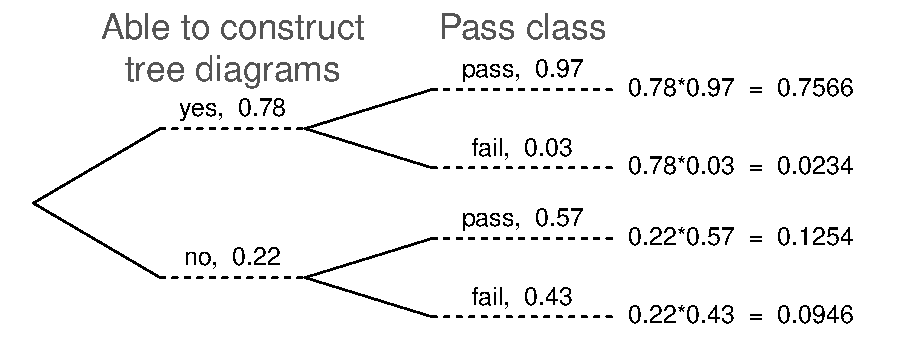
\includegraphics[width=\textwidth]{ch_probability/figures/treeDiagramAndPass/treeDiagramAndPass} \vspace{-25mm}
\end{minipage}}


%%
\subsection{Bayes' Theorem}
\label{bayesTheoremSubsection}

\index{Bayes' Theorem|(}

In many instances, we are given a conditional probability of the form
\begin{align*}
P(\text{statement about variable 1}\ |\ \text{statement about variable 2})
\end{align*}
but we would really like to know the inverted conditional probability:
\begin{align*}
P(\text{statement about variable 2}\ |\ \text{statement about variable 1})
\end{align*}
For example, instead of wanting to know $P($lived $|$ inoculated$)$, we might want to know $P($inoculated $|$ lived$)$. This is more challenging because it cannot be read directly from the tree diagram. In these instances we use \term{Bayes' Theorem}. Let's begin by looking at a new example.

\D{\newpage}

\begin{examplewrap}
\begin{nexample}{In Canada, about 0.35\% of women over 40 will develop breast cancer in any given year. A common screening test for cancer is the mammogram, but this test is not perfect. In about 11\% of patients with breast cancer, the test gives a \term{false negative}: it indicates a woman does not have breast cancer when she does have breast cancer. Similarly, the test gives a \term{false positive} in 7\% of patients who do not have breast cancer: it indicates these patients have breast cancer when they actually do not.\footnotemark If we tested a random woman over 40 for breast cancer using a mammogram and the test came back positive -- that is, the test suggested the patient has cancer -- what is the probability that the patient actually has breast cancer?}\label{probabilityOfBreastCancerGivenPositiveTestExample}
We are given sufficient information to quickly compute the probability of testing positive if a woman has breast cancer ($1.00 - 0.11 = 0.89$). However, we seek the inverted probability of cancer given a positive test result:
\begin{align*}
P(\text{has BC}\ |\ \text{mammogram$^+$})
\end{align*}
Here, ``has BC'' is an abbreviation for the patient actually having breast cancer, and ``mammogram$^+$'' means the mammogram screening was positive, which in this case means the test suggests the patient has breast cancer. (Watch out for the non-intuitive medical language: a~\emph{positive} test result suggests the possible presence of cancer in a mammogram screening.) We can use the conditional probability formula from the previous section: $P(A|B) = \frac{P(A \text{ and } B)}{P(B)}$. Our conditional probability can be found as follows:
\begin{align*}
P(\text{has BC $|$ mammogram$^+$}) &=  \frac{P(\text{has BC and mammogram$^+$})}{P(\text{mammogram$^+$})}
\end{align*}
The probability that a mammogram is positive is as follows.
\begin{align*}
P(\text{mammogram$^+$})=P(\text{has BC and mammogram$^+$}) +  P(\text{no BC and mammogram$^+$})
\end{align*}
A tree diagram is useful for identifying each probability and is shown in Figure~\ref{BreastCancerTreeDiagram}. Using the tree diagram, we find that
\begin{align*}
P(&\text{has BC $|$ mammogram$^+$}) \\
&= \frac{P(\text{has BC and mammogram$^+$})}{P(\text{has BC and mammogram$^+$}) +  P(\text{no BC and mammogram$^+$})} \\
&= \frac{0.0035(0.89)}{0.0035(0.89)+0.9965(0.07)}\\
&= \frac{0.00312}{0.07288}\approx 0.0428
\end{align*}
That is, even if a patient has a positive mammogram screening, there is still only a~4\%~chance that she has breast cancer.
\end{nexample}
\end{examplewrap}
\footnotetext{The probabilities reported here were obtained using studies reported at \oiRedirect{textbook-breastCancerDotOrg_20090831b}{www.breastcancer.org} and \oiRedirect{textbook-ncbi_nih_breast_cancer}{www.ncbi.nlm.nih.gov/pmc/articles/PMC1173421}.}

\begin{figure}[ht]
\centering
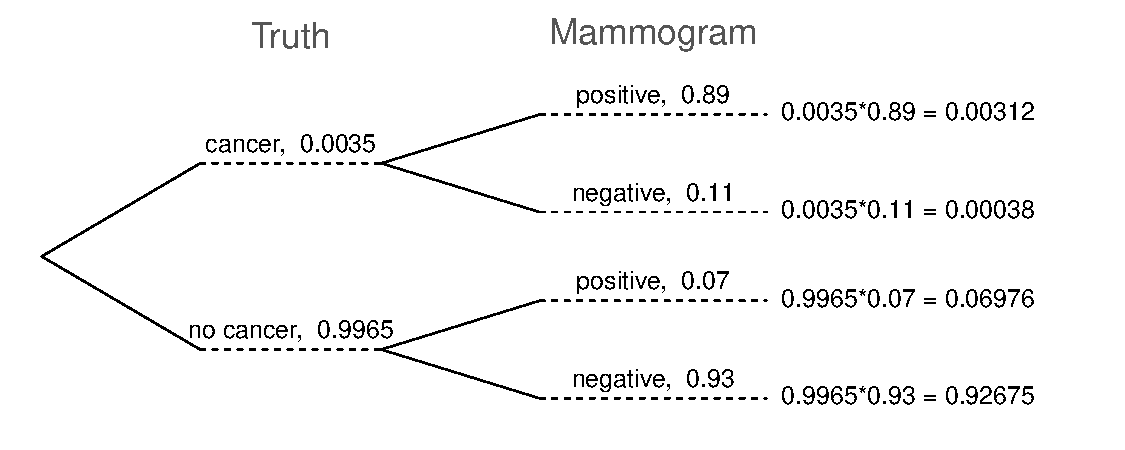
\includegraphics[width=0.9\textwidth]{ch_probability/figures/BreastCancerTreeDiagram/BreastCancerTreeDiagram}
\caption{Tree diagram for Example~\ref{probabilityOfBreastCancerGivenPositiveTestExample}, computing the probability a random patient who tests positive on a mammogram actually has breast cancer.}
\label{BreastCancerTreeDiagram}
\end{figure}

Example~\ref{probabilityOfBreastCancerGivenPositiveTestExample} highlights why doctors often run more tests regardless of a first positive test result. When a medical condition is rare, a single positive test isn't generally definitive.

\D{\newpage}

Consider again the last equation of Example~\ref{probabilityOfBreastCancerGivenPositiveTestExample}.
Using the tree diagram, we can see that the numerator (the top of the fraction) is equal to the following product:
\begin{align*}
P(\text{has BC and mammogram$^+$}) = P(\text{mammogram$^+$} | \text{ has BC})P(\text{has BC})
\end{align*}
The denominator -- the probability the screening was positive -- is equal to the sum of probabilities for each positive screening scenario:
\begin{align*}
P(\text{\underline{\color{black}mammogram$^+$}})
	&= P(\text{\underline{\color{black}mammogram$^+$} and no BC})
		+ P(\text{\underline{\color{black}mammogram$^+$} and has BC})
\end{align*}
In the example, each of the probabilities on the right side was broken down into a product of a conditional probability and marginal probability using the tree diagram.
\begin{align*}
P(\text{mammogram$^+$})
	&= P(\text{mammogram$^+$ and no BC}) + P(\text{mammogram$^+$ and has BC}) \\
	&= P(\text{mammogram$^+$} | \text{ no BC})P(\text{no BC}) \\
			   &\qquad\qquad + P(\text{mammogram$^+$} | \text{ has BC})P(\text{has BC})
\end{align*}
We can see an application of Bayes' Theorem by substituting the resulting probability expressions into the numerator and denominator of the original conditional probability.
\begin{align*}
& P(\text{has BC} | \text{ mammogram$^+$})  \\
& \qquad= \frac{P(\text{mammogram$^+$} | \text{ has BC})P(\text{has BC})}
	{P(\text{mammogram$^+$} | \text{ no BC})P(\text{no BC}) + P(\text{mammogram$^+$} | \text{ has BC})P(\text{has BC})}
\end{align*}

\begin{onebox}{Bayes' Theorem: inverting probabilities}
Consider the following conditional probability for variable 1 and variable 2:\vspace{-1.5mm}
\begin{align*}
P(\text{outcome $A_1$ of variable 1} | \text{ outcome $B$ of variable 2})
\end{align*}
Bayes' Theorem states that this conditional probability can be identified as the following fraction:\vspace{-1.5mm}
\begin{align*}
\frac{P(B | A_1) P(A_1)}
	{P(B | A_1) P(A_1) + P(B | A_2) P(A_2) + \cdots + P(B | A_k) P(A_k)}
	\label{equationOfBayesTheorem}
\end{align*}
where $A_2$, $A_3$, ..., and $A_k$ represent all other possible outcomes of the first variable.
\index{Bayes' Theorem|textbf}
\end{onebox}

\D{\newpage}

Bayes' Theorem is just a generalization of what we have done using tree diagrams. The formula need not be memorized, since it can always be derived using a tree diagram:
\begin{itemize}
\setlength{\itemsep}{0mm}
\item The numerator identifies the probability of getting both $A_1$ and $B$.
\item The denominator is the overall probability of getting $B$. Traverse each branch of the tree diagram that ends with event $B$. Add up the required products.
\end{itemize}

\begin{exercisewrap}
\begin{nexercise} \label{exerciseForParkingLotOnCampusBeingFullAndWhetherOrNotThereIsASportingEvent}
Jose visits campus every Thursday evening. However, some days the parking garage is full, often due to college events. There are academic events on 35\% of evenings, sporting events on 20\% of evenings, and no events on 45\% of evenings. When there is an academic event, the garage fills up about 25\% of the time, and it fills up 70\% of evenings with sporting events. On evenings when there are no events, it only fills up about 5\% of the time. If Jose comes to campus and finds the garage full, what is the probability that there is a sporting event? Use a tree diagram to solve this problem.\footnotetext{\begin{minipage}[t]{0.47\textwidth}
The tree diagram, with three primary branches, is shown to the right. We want
\begin{align*}
P(&\text{sporting event} | \text{garage full}) \\
&= \frac{P(\text{sporting event and garage full})}{P(\text{garage full})} \\
&=\frac{0.14}{0.0875 + 0.14 + 0.0225} = 0.56.
\end{align*}
If the garage is full, there is a 56\% probability that there is a sporting event. \vspace{0.1mm} \\\
\end{minipage}
\begin{minipage}[c]{0.5\textwidth}
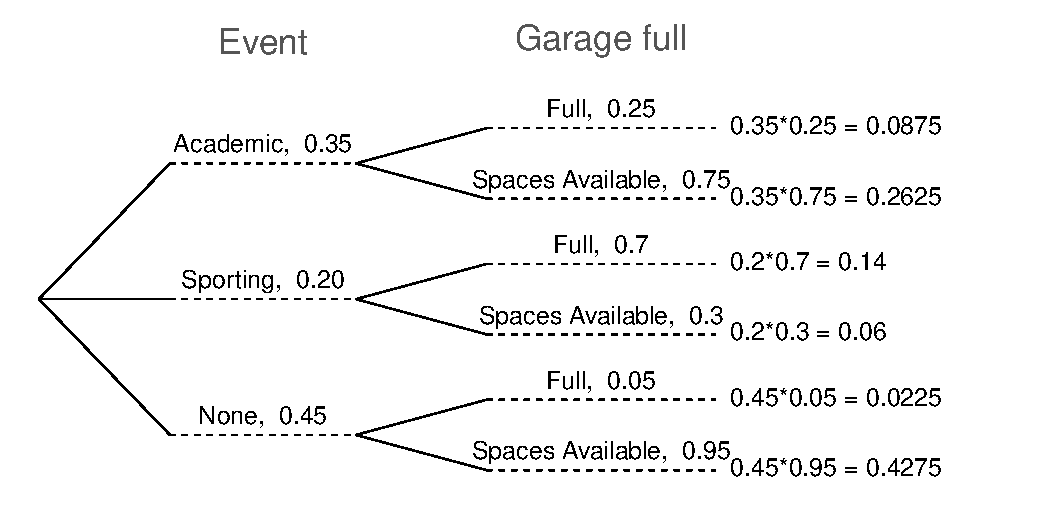
\includegraphics[width=\textwidth]{ch_probability/figures/treeDiagramGarage/treeDiagramGarage}\vspace{-30mm}
\end{minipage}}
\end{nexercise}
\end{exercisewrap}

The last several exercises offered a way to update our belief about whether there is a sporting event, academic event, or no event going on at the school based on the information that the parking lot was full. This strategy of \emph{updating beliefs} using Bayes' Theorem is actually the foundation of an entire section of statistics called \term{Bayesian statistics}. While Bayesian statistics is very important and useful, we will not have time to cover it in this book.

\index{Bayes' Theorem|)}
\index{tree diagram|)}
\index{conditional probability|)}
\index{probability|)}


\D{\newpage}

%%
\subsection*{Section summary}

\begin{itemize}

\item A \term{conditional probability} can be written as $P(A | B)$ and is read, ``Probability of $A$ given $B$".  $P(A|B)$ is the probability of $A$, given that $B$ has occurred.  In a conditional probability, we are given some information.  In an \term{unconditional probability}, such as $P(A)$, we are not given any information.

\item Sometimes $P(A | B)$ can be deduced.  For example, when drawing without replacement from a deck of cards, $P(\text{2nd draw is an Ace }| \text{ 1st draw was an Ace}) = \frac{3}{51}$.  When this is not the case, as when working with a table or a Venn diagram, one must use the conditional probability rule $P(A | B) = \frac{P(A\text{ and }B)}{P(B)}$.

\item In the last section, we saw that two events are \term{independent} when the outcome of one has no effect on the outcome of the other.  When $A$ and $B$ are independent, $P(A | B) = P(A)$.

\item When $A$ and $B$  are \term{dependent}, find the probability of $A$ \emph{and} $B$ using the \term{General Multiplication Rule}:
$P(A \text{ and } B) = P(A | B)\times P(B)$.

\item In the \emph{special case} where $A$ and $B$ are \term{independent}, $P(A \text{ and } B) = P(A)\times P(B)$.

\item If $A$ and $B$ are \term{mutually exclusive}, they must be \term{dependent}, since the occurrence of one of them changes the probability that the other occurs to 0.

\item When sampling \term{without replacement}, such as drawing cards from a deck, make sure to use \termsub{conditional probabilities}{conditional probability} when solving \emph{and} problems.  


\item Sometimes, the conditional probability $P(B|A)$ may be known, but we are interested in the ``inverted" probability $P(A|B)$.  \term{Bayes' Theorem} helps us solve such conditional probabilities that cannot be easily answered.  However, rather than memorize Bayes' Theorem, one can generally draw a tree diagram and apply the conditional probability rule $P(A | B)=\frac{P(A\text{ and }B)}{P(B)}$.  The resulting answer often has the form $\frac{w\times x\text{ }  +\text{ } y\times z}{w\times x}$, where $w, x, y, z$ are numbers from a tree diagram.


\end{itemize} 

%%%%%%%%%Section Exercises
{\exercisesheader{}

% 13 - joint_cond

\eoce{\qt{Joint and conditional probabilities\label{joint_cond}} P(A) = 0.3, 
P(B) = 0.7
\begin{parts}
\item Can you compute P(A and B) if you only know P(A) and P(B)?
\item Assuming that events A and B arise from independent random processes,
\begin{subparts}
\item what is P(A and B)?
\item what is P(A or B)?
\item what is P(A$|$B)?
\end{subparts}
\item If we are given that P(A and B) = 0.1, are the random variables giving rise 
to events A and B independent?
\item If we are given that P(A and B) = 0.1, what is P(A$|$B)?
\end{parts}
}{}

% 14 - pbj

\eoce{\qt{PB \& J\label{pbj}} Suppose 80\% of people like peanut butter, 89\% 
like jelly, and 78\% like both. Given that a randomly sampled person likes peanut 
butter, what's the probability that he also likes jelly?
}{}

% 15 - global_warming

\eoce{\qt{Global warming\label{global_warming}} \videosolution{ahss_eoce_sol-global_warming}  A Pew Research poll asked 
1,306 Americans ``From what you've read and heard, is there solid evidence that 
the average temperature on earth has been getting warmer over the past few 
decades, or not?". The table below shows the distribution of responses by party 
and ideology, where the counts have been replaced with relative frequencies.
\footfullcite{globalWarming}
\begin{center}
\begin{tabular}{ll  ccc c} 
                    &                           & \multicolumn{3}{c}{\textit{Response}} \\
\cline{3-5}
                    &                           & Earth is  & Not       & Don't Know    &   \\
                    &                           & warming   & warming   & Refuse        & Total\\
\cline{2-6}
                    & Conservative Republican   & 0.11      & 0.20      & 0.02      & 0.33  \\
\textit{Party and}  & Mod/Lib Republican        & 0.06      & 0.06      & 0.01      & 0.13 \\
\textit{Ideology}   & Mod/Cons Democrat         & 0.25      & 0.07      & 0.02      & 0.34 \\
                    & Liberal Democrat          & 0.18      & 0.01      & 0.01      & 0.20\\
\cline{2-6}
                    &Total                      & 0.60      & 0.34      & 0.06      & 1.00
\end{tabular}
\end{center}
\begin{parts}
\item Are believing that the earth is warming and being a liberal Democrat mutually 
exclusive?
\item What is the probability that a randomly chosen respondent believes the 
earth is warming or is a liberal Democrat?
\item What is the probability that a randomly chosen respondent believes the 
earth is warming given that he is a liberal Democrat?
\item What is the probability that a randomly chosen respondent believes the 
earth is warming given that he is a conservative Republican?
\item Does it appear that whether or not a respondent believes the earth is 
warming is independent of their party and ideology? Explain your reasoning.
\item What is the probability that a randomly chosen respondent is a 
moderate/liberal Republican given that he does not believe that the earth is 
warming? 
\end{parts}
}{}

\D{\newpage}
% 16 - health_coverage_rel_freqs

\eoce{\qt{Health coverage, relative frequencies\label{health_coverage_rel_freqs}} 
The Behavioral Risk Factor Surveillance System (BRFSS) is an annual telephone 
survey designed to identify risk factors in the adult population and report 
emerging health trends. The following table displays the distribution of health 
status of respondents to this survey (excellent, very good, good, fair, poor) 
and whether or not they have health insurance.
\begin{center}
\begin{tabular}{rrrrrrrr}
& &  \multicolumn{5}{c}{\textit{Health Status}} &  \\ 
\cline{3-7}
                    &       & Excellent & Very good & Good      & Fair      & Poor      & Total \\ 
\cline{2-8}
\textit{Health}     & No    & 0.0230    & 0.0364    & 0.0427    & 0.0192    & 0.0050    & 0.1262 \\ 
\textit{Coverage}   & Yes   & 0.2099    & 0.3123    & 0.2410    & 0.0817    & 0.0289    & 0.8738 \\ 
\cline{2-8}
                    & Total & 0.2329    & 0.3486    & 0.2838    & 0.1009    & 0.0338    & 1.0000
\end{tabular}
\end{center}
\begin{parts}
\item Are being in excellent health and having health coverage mutually 
exclusive?
\item What is the probability that a randomly chosen individual has excellent 
health?
\item What is the probability that a randomly chosen individual has excellent 
health given that he has health coverage?
\item What is the probability that a randomly chosen individual has excellent 
health given that he doesn't have health coverage?
\item Do having excellent health and having health coverage appear to be 
independent?
\end{parts}
}{}

% 17 - marbles_in_urn

\eoce{\qt{Marbles in an urn\label{marbles_in_urn}} Imagine you have an urn 
containing 5 red, 3 blue, and 2 orange marbles in it. 
\begin{parts}
\item What is the probability that the first marble you draw is blue?
\item Suppose you drew a blue marble in the first draw. If drawing with 
replacement, what is the probability of drawing a blue marble in the second draw?
\item Suppose you instead drew an orange marble in the first draw. If drawing 
with replacement, what is the probability of drawing a blue marble in the second 
draw?
\item If drawing with replacement, what is the probability of drawing two blue 
marbles in a row?
\item When drawing with replacement, are the draws independent? Explain.
\end{parts}
}{}

% 18 - socks_in_drawer

\eoce{\qt{Socks in a drawer\label{socks_in_drawer}} In your sock drawer you have 
4 blue, 5 gray, and 3 black socks. Half asleep one morning you grab 2 socks at 
random and put them on. Find the probability you end up wearing
\begin{parts}
\item 2 blue socks
\item no gray socks
\item at least 1 black sock
\item a green sock
\item matching socks
\end{parts}
}{}

% 19 - chips_in_bag

\eoce{\qt{Chips in a bag\label{chips_in_bag}} Imagine you have a bag 
containing 5 red, 3 blue, and 2 orange chips.
\begin{parts}
\item Suppose you draw a chip and it is blue. If drawing without replacement, 
what is the probability the next is also blue?
\item Suppose you draw a chip and it is orange, and then you draw a second chip 
without replacement. What is the probability this second chip is blue?
\item If drawing without replacement, what is the probability of drawing two blue 
chips in a row?
\item When drawing without replacement, are the draws independent? Explain.
\end{parts}
}{}

% 20 - books_on_shelf

\eoce{\qt{Books on a bookshelf\label{books_on_shelf}} The table below shows the 
distribution of books on a bookcase based on whether they are nonfiction or 
fiction and hardcover or paperback.
\begin{center}
\begin{tabular}{ll  cc c} 
                                &           & \multicolumn{2}{c}{\textit{Format}} \\
\cline{3-4}
                                &           & Hardcover     & Paperback     & Total \\
\cline{2-5}
\multirow{2}{*}{\textit{Type}}  & Fiction   & 13            & 59            & 72 \\
                                & Nonfiction& 15            & 8             & 23 \\
\cline{2-5} 
                                & Total     & 28            & 67            & 95 \\
\cline{2-5}
\end{tabular}
\end{center}
\begin{parts}
\item Find the probability of drawing a hardcover book first then a paperback 
fiction book second when drawing without replacement.
\item Determine the probability of drawing a fiction book first and then a 
hardcover book second, when drawing without replacement.
\item Calculate the probability of the scenario in part~(b), except this time 
complete the calculations under the scenario where the first book is placed back 
on the bookcase before randomly drawing the second book.
\item The final answers to parts~(b) and~(c) are very similar. Explain why this 
is the case.
\end{parts}
}{}

% 21 - student_outfits

\eoce{\qt{Student outfits\label{student_outfits}} \videosolution{ahss_eoce_sol-student_outfits} In a classroom with 24 
students, 7 students are wearing jeans, 4 are wearing shorts, 8 are wearing 
skirts, and the rest are wearing leggings. If we randomly select 3 students 
without replacement, what is the probability that one of the selected students is 
wearing leggings and the other two are wearing jeans? Note that these are 
mutually exclusive clothing options.
}{}

% 22 - birthday_problem

\eoce{\qt{The birthday problem\label{birthday_problem}} Suppose we pick three 
people at random. For each of the following questions, ignore the special case 
where someone might be born on February 29th, and assume that births are evenly 
distributed throughout the year.
\begin{parts}
\item What is the probability that the first two people share a birthday? 
\item What is the probability that at least two people share a birthday?
\end{parts}
}{}

% 23 - tree_drawing_box_plots

\eoce{\qt{Drawing box plots\label{tree_drawing_box_plots}} After an introductory 
statistics course, 80\% of students can successfully construct box plots. Of 
those who can construct box plots, 86\% passed, while only 65\% of those students 
who could not construct box plots passed.
\begin{parts}
\item Construct a tree diagram of this scenario.
\item Calculate the probability that a student is able to construct a box plot 
if it is known that he passed.
\end{parts}
}{}

% 24 - tree_thrombosis

\eoce{\qt{Predisposition for thrombosis\label{tree_thrombosis}} A genetic test is 
used to determine if people have a predisposition for \textit{thrombosis}, which 
is the formation of a blood clot inside a blood vessel that obstructs the flow of 
blood through the circulatory system. It is believed that 3\% of people actually 
have this predisposition. The genetic test is 99\% accurate if a person actually 
has the predisposition, meaning that the probability of a positive test result 
when a person actually has the predisposition is 0.99. The test is 98\% accurate 
if a person does not have the predisposition. What is the probability that a 
randomly selected person who tests positive for the predisposition by the test 
actually has the predisposition?
}{}

% 25 - tree_lupus

\eoce{\qt{It's never lupus\label{tree_lupus}} \videosolution{ahss_eoce_sol-tree_lupus} Lupus is a medical phenomenon where 
antibodies that are supposed to attack foreign cells to prevent infections 
instead see plasma proteins as foreign bodies, leading to a high risk of blood 
clotting. It is believed that 2\% of the population suffer from this disease. The 
test is 98\% accurate if a person actually has the disease. The test is 74\% 
accurate if a person does not have the disease. There is a line from the Fox 
television show \emph{House} that is often used after a patient tests positive 
for lupus: ``It's never lupus." Do you think there is truth to this statement? 
Use appropriate probabilities to support your answer.
}{}

% 26 - tree_exit_poll

\eoce{\qt{Exit poll\label{tree_exit_poll}} Edison Research gathered exit poll 
results from several sources for the Wisconsin recall election of Scott Walker. 
They found that 53\% of the respondents voted in favor of Scott Walker. 
Additionally, they estimated that of those who did vote in favor for Scott 
Walker, 37\% had a college degree, while 44\% of those who voted against Scott 
Walker had a college degree. Suppose we randomly sampled a person who 
participated in the exit poll and found that he had a college degree. What is the 
probability that he voted in favor of Scott Walker?
\footfullcite{data:scott}
}{}
}





%______________________________________________
\section[The binomial formula]{The binomial formula }
\label{binomialForm}

\sectionintro{
\noindent%
What is the probability of exactly 50 heads in
100 coin tosses?
Or the probability of randomly sampling 8 people and having
exactly 1 of them be left-handed?
Or of at most 3~people exceeding their insurance deductible
in a random sample of 20 people?
The binomial formula can help us answer these questions.


%%
\subsection*{Learning objectives}
\begin{enumerate}
\setlength{\itemsep}{0mm}
\item Calculate the number of possible scenarios for obtaining $x$ successes in $n$ trials.

\item Determine whether a scenario is binomial or not.

\item Calculate the probability of obtaining exactly $x$ successes in $n$ independent trials.  

\item Recognize that the binomial formula uses the special Addition Rule for mutually exclusive events.

\item Find probabilities of the form ``at least” or ``at most” by applying the binomial formula multiple times.

\end{enumerate}
}

%%
\subsection{Introducing the binomial formula}

\newcommand{\insureSprob}{0.7}
\newcommand{\insureSperc}{70\%}
\newcommand{\insureFprob}{0.3}
\newcommand{\insureFperc}{30\%}
\newcommand{\insureDistA}{0.7}
\newcommand{\insureDistB}{0.21}
\newcommand{\insureDistC}{0.063}
\newcommand{\insureDistD}{0.019}
\newcommand{\insureDistE}{0.006}
\newcommand{\insureCDistA}{0.7}
\newcommand{\insureCDistB}{0.91}
\newcommand{\insureCDistC}{0.973}
\newcommand{\insureCDistCComplement}{0.027}
\newcommand{\insureCDistD}{0.992}
\newcommand{\insureCDistE}{0.998}
\newcommand{\insureGeomMean}{1.43}
\newcommand{\insureS}{\resp{not}}
\newcommand{\insureF}{\resp{exceed}}
% Doesn't consider binomial coefficient in next calculated value.
\newcommand{\insureBinomCinDSingleScenario}{0.103}
\newcommand{\insureBinomCinD}{0.412}
\newcommand{\insureBinomEinHSingleScenario}{0.00454}
\newcommand{\insureBinomEinH}{0.254}
\newcommand{\insureBinomFourtyExpValue}{28}
\newcommand{\insureBinomFourtySD}{2.9}
\newcommand{\insureBinomFourtyLower}{22}
\newcommand{\insureBinomFourtyUpper}{34}

Many health insurance plans in the United States have
a deductible, where the insured individual is responsible
for costs up to the deductible, and then the costs above
the deductible are shared between the individual and
insurance company for the remainder of the year.

Suppose a health insurance company found that \insureSperc{} of the
people they insure stay below their deductible in any given year.
Each of these people can be thought of as a \term{trial}.
We label a person a \term{success} if her healthcare costs
do not exceed the deductible.
We label a person a \term{failure} if she does exceed her
deductible in the year.
Because 70\% of the individuals will not hit their deductible,
we denote the \term{probability of a success} as
$p = \insureSprob{}$.


\begin{examplewrap}
\begin{nexample}{Suppose the insurance agency is considering
    a random sample of four individuals they insure.
    What is the chance exactly one of them will exceed
    the deductible and the other three will not?
    Let's call the four people
    Ariana ($A$),
    Brittany ($B$),
    Carlton ($C$),
    and Damian ($D$)
    for convenience.}
  \label{insureOneOfFourExceedsDeductible}%
  Let's consider a scenario where one person exceeds
  the deductible:
  \begin{align*}
  &P(A=\text{\insureF{}},
      \text{ }B=\text{\insureS{}},
      \text{ }C=\text{\insureS{}},
      \text{ }D=\text{\insureS{}}) \\
    &\quad = P(A=\text{\insureF{}})\ 
        P(B=\text{\insureS{}})\ 
        P(C=\text{\insureS{}})\ 
        P(D=\text{\insureS{}}) \\
    &\quad =  (\insureFprob{})
        (\insureSprob{})
        (\insureSprob{})
        (\insureSprob{}) \\
    &\quad = (\insureSprob{})^3 (\insureFprob{})^1 \\
    &\quad = \insureBinomCinDSingleScenario{}
  \end{align*}
  But there are three other scenarios: Brittany, Carlton,
  or Damian could have been the one to exceed the deductible.
  In each of these cases, the probability is again
  $(\insureSprob{})^3 (\insureFprob{})^1$.
  These four scenarios exhaust all the possible ways that
  exactly one of these four people could have exceeded
  the deductible, so the total probability is
  $4 \times (\insureSprob{})^3 (\insureFprob{})^1
      = \insureBinomCinD{}$.
\end{nexample}
\end{examplewrap}

\begin{exercisewrap}
\begin{nexercise}
Verify that the scenario where Brittany is the only one to exceed the deductible has probability
$(\insureSprob{})^3 (\insureFprob{})^1$.~\footnotemark{}
\end{nexercise}
\end{exercisewrap}
\footnotetext{
  $P(A=\text{\insureS{}},
      \text{ }B=\text{\insureF{}},
      \text{ }C=\text{\insureS{}},
      \text{ }D=\text{\insureS{}})
    = (\insureSprob{})(\insureFprob{})
        (\insureSprob{})(\insureSprob{})
    = (\insureSprob{})^3 (\insureFprob{})^1$.}


The binomial distribution describes the probability of having exactly $x$ successes
in $n$ independent trials with probability
of a success $p$
(in Example~\ref{insureOneOfFourExceedsDeductible},
$n=4$, $x=3$, $p=\insureSprob{}$).
We would like to determine the probabilities associated
with the binomial distribution more generally,
i.e. we want a formula where we can use $n$, $x$, and $p$
to obtain the probability.
To do this, we reexamine each part of
Example~\ref{insureOneOfFourExceedsDeductible}.

There were four individuals who could have been the one
to exceed the deductible, and each of these four scenarios
had the same probability.
Thus, we could identify the final probability as
\begin{align*}
[\text{\# of scenarios}] \times P(\text{single scenario})
\end{align*}
The first component of this equation is the number of ways
to arrange the $x=3$ successes among the $n=4$ trials.
The second component is the probability of any of the four
(equally probable) scenarios.

Consider $P($single scenario$)$ under the general case of
$x$ successes and $n-x$ failures in the $n$ trials.
In any such scenario, we apply the Multiplication Rule
for independent events:
\begin{align*}
p^x (1 - p)^{n - x}
\end{align*}
This is our general formula for $P($single scenario$)$.

Secondly, we introduce the \term{binomial coefficient}, which gives the number
of ways to choose $x$ successes in $n$ trials,
i.e. arrange $x$ successes and $n - x$ failures:
\begin{align*}
{n\choose x} = \frac{n!}{x! (n - x)!}
\end{align*}
The quantity ${n\choose x}$ is read
\term{n choose x}.\footnote{Other notations for
  $n$ choose $x$ includes $_nC_x$, $C_n^x$, and $C(n,x)$.}
The exclamation point notation (e.g. $n!$) denotes
a \term{factorial} expression.
\begin{align*}
& 0! = 1 \\
& 1! = 1 \\
& 2! = 2\times1 = 2 \\
& 3! = 3\times2\times1 = 6 \\
& 4! = 4\times3\times2\times1 = 24 \\
& \vdots \\
& n! = n\times(n-1)\times...\times3\times2\times1
\end{align*}
Using the formula, we can compute the number of ways
to choose $x = 3$ successes in $n = 4$ trials:
\begin{align*}
{4 \choose 3} = \frac{4!}{3!(4-3)!}
  = \frac{4!}{3!1!} 
  = \frac{4\times3\times2\times1}{(3\times2\times1) (1)}
  = 4
\end{align*}
This result is exactly what we found by carefully thinking
of each possible scenario in
Example~\ref{insureOneOfFourExceedsDeductible}.

Substituting $n$ choose $x$ for the number of scenarios
and $p^x(1-p)^{n-x}$ for the single scenario probability
yields the \term{binomial formula}.

\D{\newpage}

\begin{onebox}{Binomial formula}
Suppose the probability of a single trial being a success is $p$. Then the probability of observing exactly $x$ successes in $n$ independent trials is given by\vspace{-1mm}
\begin{eqnarray*}
P(X=x)={n\choose x}p^x(1-p)^{n-x} = \frac{n!}{x!(n-x)!}p^x(1-p)^{n-x}
\label{binomialFormula}
\end{eqnarray*}
\end{onebox}


%%
\subsection{When and how to apply the formula}

\begin{onebox}{Is it binomial? Four conditions to check.}
  \label{isItBinomialTipBox}%
  (1) The trials are independent. \\
  (2) The number of trials, $n$, is fixed. \\
  (3) Each trial outcome can be classified as a \emph{success}
      or \emph{failure}. \\
  (4) The probability of a success, $p$, is the same for
      each trial.
\end{onebox}

\begin{examplewrap}
\begin{nexample}{What is the probability that 3 of 8 randomly
    selected individuals will have exceeded the insurance
    deductible, i.e. that 5 of 8 will not exceed the deductible?
    Recall that 70\% of individuals will not exceed the
    deductible.}
  We would like to apply the binomial model,
  so we check the conditions.
  The number of trials is fixed ($n = 8$) (condition 2)
  and each trial outcome can be classified as a success
  or failure (condition 3).
  Because the sample is random, the trials are independent
  (condition~1) and the probability of a success is the same
  for each trial (condition~4).

  In the outcome of interest, there are $x = 5$ successes
  in $n = 8$ trials (recall that a success is an individual
  who does \emph{not} exceed the deductible, and the
  probability of a success is $p = \insureSprob{}$.
  So the probability that 5 of 8 will not exceed the
  deductible and 3 will exceed the deductible is given by
  \begin{align*}
  { 8 \choose 5}(\insureSprob{})^5
  (1-\insureSprob{})^{8-5}
    &= \frac{8!}{5!(5-3)!}
        (\insureSprob{})^5(1-\insureSprob{})^{8-5} \\
    &= \frac{8!}{5!3!}
        (\insureSprob{})^5(\insureFprob{})^3
  \end{align*}
  Dealing with the factorial part:
  \begin{align*}
  \frac{8!}{5!3!}
    = \frac{8\times7\times6\times5\times4\times3\times2\times1}
        {(5\times4\times3\times2\times1)(3\times2\times1)}
    = \frac{8\times7\times6}{3\times2\times1}
    = 56
  \end{align*}
  Using $(\insureSprob{})^5(\insureFprob{})^3
    \approx \insureBinomEinHSingleScenario{}$,
  the final probability is about
  $56\times \insureBinomEinHSingleScenario{}
    \approx \insureBinomEinH{}$.
\end{nexample}
\end{examplewrap}


  If you must calculate the binomial coefficient by hand, it's often useful
  to cancel out as many terms as possible in the top and
  bottom.  See Section~\ref{calculatorBinomial} for how to evaluate the binomial coefficient and the binomial formula using a calculator.

\begin{onebox}{Computing binomial probabilities}
  The first step in using the binomial model is to check
  that the model is appropriate.
  The second step is to identify $n$, $p$, and $x$.
  Finally, apply the binomial formula to determine the probability and interpret the results.%
  \vspace{3mm}

\end{onebox}



%%%%%%%
\begin{examplewrap}
\begin{nexample}{Approximately 35\% of a population has blood type O+.  Suppose four people show up at a hospital and we want to find the probability that exactly one of them has blood type O+.  Can we use the binomial formula?  }
To check if the binomial model is appropriate,
  we must verify the conditions.
\begin{enumerate}
\setlength{\itemsep}{0mm}
\item If we suppose that these 4 people comprise a random sample, then we can treat them as independent.  This seems reasonable, since one person with a particular blood type showing up at a hospital seems unlikely to affect the chance that other people with that blood type would show up at the hospital.  
\item We have a fixed number of trials ($n=4$).
\item Each outcome is a success or failure (blood type O+ or not blood type O+).
\item The probability of a success is the same for each
  trial  since the individuals are like a random sample
  ($p=0.35$ if we say a ``success'' is someone having blood type O+).
\end{enumerate}
\end{nexample}
\end{examplewrap}

 \begin{exercisewrap}
\begin{nexercise}
The probability that a random smoker will develop a severe
lung condition in his or her lifetime is about $0.3$.
If you have 4 friends who smoke and you want to find the probability that 1 of them will develop a severe lung condition in his or her lifetime, can you apply the binomial formula?\footnotemark{}
\end{nexercise}
\end{exercisewrap}
\footnotetext{While conditions (2) and (3) are met, most likely the friends know each other, so the independence
  assumption (1) is probably not satisfied.
  For example, acquaintances may have similar smoking habits,
  or those friends might make a pact to quit together.  Condition (4) is also not satisfied since this is not a random sample of people.}


\begin{examplewrap}
\begin{nexample}
{Given that 35\% of a population has blood type O+, what is the probabilty that in a random sample of 4 people:  
\begin{enumerate}[(a)]
\setlength{\itemsep}{0mm}
\item
    none of them have blood type O+?
\item
    one will have blood type O+?
\item
    no more than one will have blood type O+?
\end{enumerate}
}
  Compute parts~(a) and~(b) using the binomial formula:
\begin{enumerate}[(a)]
\item
  $P(X=0)
    = {4 \choose 0} (0.35)^0 (0.65)^4
    = 1\times1\times 0.65^4 = 0.65^4
    = 0.179$\\
Note that we could have answered this question without the binomial formula, using methods from the previous section.
\item 
  $P(X=1)
    = {4 \choose 1} (0.35)^1(0.65)^{3}
    = 0.384$.
  \item This can be computed as the sum of parts~(a) and~(b):
  $P(X=0) + P(X=1) = 0.179 + 0.384 = 0.563$.
  That is, there is about a 56.3\% chance that no more than
  one of them will have blood type O+.
\end{enumerate}
\label{bloodTypeOPos}
\end{nexample}
\end{examplewrap}

\D{\newpage}

\begin{exercisewrap}
\begin{nexercise}
What is the probability that at least 3 of 4 people in a random sample will have blood type O+ if 35\% of the population has blood type O+?\footnotemark
\end{nexercise}
\end{exercisewrap}
\footnotetext{$P(\text{at least 3 of 4 have blood type O+})
      = P(X=3) + P(X=4) = {4 \choose 3} (0.35)^3 (0.65)^1+(0.35)^4= 0.111 + 0.015 = 0.126$}





\begin{examplewrap}
\begin{nexample}{There are 13 marbles in a bag. 4 are blue and 9 are red. Randomly draw 5 marbles \emph{without replacement}. Find the probability you get exactly 3 blue marbles.}Because the probability of success $p$ is not the same for each trial, we cannot use the binomial formula. However, we can use the same logic to arrive at the following answer. 
\begin{align*}
P(X = 3) &= (\text{\# of combinations with 3 blue})\times P(\text{3 blue and 2 red in a \emph{specific} order}) \\
&={5\choose 3}\times P(\text{BBBRR}) \\
&= {5\choose 3}\left(\frac{4}{13}\times \frac{3}{12}\times \frac{2}{11} \times \frac{9}{10} \times \frac{8}{9}\right) \\
&= 0.1119
\end{align*}
\end{nexample}
\end{examplewrap}

\begin{exercisewrap}
\begin{nexercise}
{Draw 4 cards without replacement from a deck of 52 cards.  What is the probability that you get at least two hearts?}\footnotemark
\end{nexercise}
\end{exercisewrap}
\footnotetext{$P\text{(at least 2 hearts in 4 draws from a deck)} = 1 - [P(X=0) + P(X=1)] = 1 - [(\frac{39}{52})(\frac{38}{51})(\frac{37}{50})(\frac{36}{49}) + {4 \choose 1}(\frac{13}{52})(\frac{39}{51})(\frac{38}{50})(\frac{37}{49})] = 1 - [.0.3038 + 0.4388] = 0.2574$.
}

Lastly, we consider the binomial coefficient,,
$n$ choose $x$, under some special scenarios.

\begin{exercisewrap}
\begin{nexercise}
Why is it true that ${n \choose 0}=1$ and ${n \choose n}=1$
for any number $n$?\footnotemark{}
\end{nexercise}
\end{exercisewrap}
\footnotetext{Frame these expressions into words.
  How many different ways are there to arrange 0 successes
  and $n$ failures in $n$ trials?
  (1 way.)
  How many different ways are there to arrange $n$ successes
  and 0 failures in $n$ trials?
  (1 way.)}

\begin{exercisewrap}
\begin{nexercise}
How many ways can you arrange one success and $n-1$ failures
in $n$ trials?
How many ways can you arrange $n-1$ successes and one failure
in $n$ trials?\footnotemark{}
\end{nexercise}
\end{exercisewrap}
\footnotetext{One success and $n-1$ failures:
  there are exactly $n$ unique places we can put
  the success, so there are $n$ ways to arrange one
  success and $n-1$ failures.
  A~similar argument is used for the second question.
  Mathematically, we show these results by verifying
  the following two equations:
  \begin{align*}
  {n \choose 1} = n,
    \qquad {n \choose n-1} = n
  \end{align*}}


\D{\newpage}

%%
\subsection{Calculator: binomial probabilities}
\label{calculatorBinomial}

\begin{onebox}{\videohref{ti84_binomial_coefficient} TI-83/84: Computing the binomial coefficient \MakeLowercase{\pmb{${n\choose x}$}}}
Use \calctext{MATH}, \calctext{PRB}, \calctext{nCr} to evaluate $n$ choose $r$. Here $r$ and $x$ are different letters for the same quantity.
\begin{enumerate}
\setlength{\itemsep}{0mm}
\item Type the value of $n$.
\item Select \calctext{MATH}.
\item Right arrow to \calctext{PRB}.
\item Choose \calctext{3:nCr}.
\item Type the value of $x$.
\item Hit \calcbutton{ENTER}.
\end{enumerate}
Example: \calctext{5 nCr 3} means {5 choose 3}.\end{onebox}

\begin{onebox}{\videohref{casio_binomial_coefficient} Casio fx-9750GII: Computing the binomial coefficient \MakeLowercase{\pmb{${n\choose x}$}}}
\begin{enumerate}
\setlength{\itemsep}{0mm}
\item Navigate to the \calctext{RUN-MAT} section (hit \calcbutton{MENU}, then hit \calcbutton{1}).
\item Enter a value for $n$.
\item Go to \calctext{CATALOG} (hit buttons \calcbutton{SHIFT} and then \calcbutton{7}).
\item Type \calctext{C} (hit the \calcbutton{ln} button), then navigate down to the bolded \calctext{\textbf{C}} and hit \calcbutton{EXE}.
\item Enter the value of $x$. Example of what it should look like: \calctext{7\textbf{C}3}.
\item Hit \calcbutton{EXE}.
\end{enumerate}
\end{onebox}

\begin{onebox}{\videohref{ti84_binomial_formula} TI-84: Computing the binomial formula, \pmb{$P(X = \MakeLowercase{x)={n\choose x}p^x(1-p)^{n-x}}$}}
\label{binomialformula}
Use \calcbutton{2ND} \calcbutton{VARS}, \calctext{binompdf} to evaluate the probability of \emph{exactly} $x$ occurrences out of $n$ independent trials of an event with probability $p$. 
\begin{enumerate}
\setlength{\itemsep}{0mm}
\item Select \calcbutton{2ND} \calcbutton{VARS} (i.e. \calctext{DISTR})
\item Choose \calctext{A:binompdf} (use the down arrow to scroll down).
\item Let \calctext{trials} be $n$.
\item Let \calctext{p} be $p$
\item Let \calctext{x value} be $x$.
\item Select \calctext{Paste} and hit \calcbutton{ENTER}.\vspace{-1.5mm}
\end{enumerate}
TI-83: Do step 1, choose \calctext{0:binompdf}, then enter $n$, $p$, and $x$ separated by commas:\\
	\calctext{binompdf(n,~p,~x)}. Then hit \calcbutton{ENTER}. 
\end{onebox}

\begin{onebox}{\videohref{ti84_binomial_cdf} TI-84: Computing \pmb{$P(X \le \MakeLowercase{x)= {n\choose 0}p^0(1-p)^{n-0} + ... + {n\choose x}p^x(1-p)^{n-x}}$} }
\label{binomialcumulative}
Use \calcbutton{2ND} \calcbutton{VARS}, \calctext{binomcdf} to evaluate the cumulative probability of \emph{at most} $x$ occurrences out of $n$ independent trials of an event with probability $p$. 
\begin{enumerate}
\setlength{\itemsep}{0mm}
\item Select \calcbutton{2ND} \calcbutton{VARS} (i.e. \calctext{DISTR})
\item Choose \calctext{B:binomcdf} (use the down arrow).
\item Let \calctext{trials} be $n$.
\item Let \calctext{p} be $p$
\item Let \calctext{x value} be $x$.
\item Select \calctext{Paste} and hit \calcbutton{ENTER}.\vspace{-1.5mm}
\end{enumerate}
TI-83: Do steps 1-2, then enter the values for $n$, $p$, and $x$ separated by commas as follows: \calctext{binomcdf(n,~p,~x)}. Then hit \calctext{ENTER}.\end{onebox}


\begin{onebox}{\videohref{casio_binomial_calculations} Casio fx-9750GII: Binomial calculations}
\begin{enumerate}
\setlength{\itemsep}{0mm}
\item Navigate to \calctext{STAT} (\calcbutton{MENU}, then hit \calcbutton{2}).
\item Select \calctext{DIST} (\calcbutton{F5}), and then \calctext{BINM} (\calcbutton{F5}).
\item Choose whether to calculate the binomial distribution for a specific number of successes, $P(X = k)$, or for a range $P(X \leq k)$ of values (0~successes, 1~success, ..., $x$~successes).\vspace{-1.5mm}
  \begin{itemize}
  \setlength{\itemsep}{0mm}
  \item For a specific number of successes, choose \calctext{Bpd} (\calcbutton{F1}). %, which stands for \emph{binomial probability distribution}.
  \item To consider the range 0, 1, ..., $x$ successes, choose \calctext{Bcd}(\calcbutton{F1}). %, which stands for \emph{binomial cumulative distribution}.
  \end{itemize}
\item If needed, set \calctext{Data} to \calctext{Variable} (\calctext{Var} option, which is \calcbutton{F2}).
\item Enter the value for \calctext{x} ($x$), \calctext{Numtrial} ($n$), and \calctext{p} (probability of a success).
\item Hit \calctext{EXE}.
\end{enumerate}
\end{onebox}

\begin{exercisewrap}
\begin{nexercise}
Find the number of ways of arranging 3 blue marbles and 2 red marbles.\footnotemark
\end{nexercise}
\end{exercisewrap}
\footnotetext{Here \calctext{$n$} = 5 and \calctext{$x$} = 3.  Doing 5 \calctext{nCr} 3 gives the number of combinations as 10.}

\begin{exercisewrap}
\begin{nexercise}There are 13 marbles in a bag. 4 are blue and 9 are red. Randomly draw 5 marbles \emph{with replacement}. Find the probability you get exactly 3 blue marbles.\footnotemark
\end{nexercise}
\end{exercisewrap}
\footnotetext{Here, $n$ = 5, $p$ = 4/13, and $x$ = 3, so set \calctext{trials} = 5, \calctext{p} = 4/13 and \calctext{x value} = 3.  The probability is 0.1396.}

\begin{exercisewrap}
\begin{nexercise}There are 13 marbles in a bag. 4 are blue and 9 are red. Randomly draw 5 marbles \emph{with replacement}. Find the probability you get \emph{at most} 3 blue marbles (i.e. less than or equal to 3 blue marbles).\footnotemark\end{nexercise}
\end{exercisewrap}
\footnotetext{Similarly, set \calctext{trials} = 5, \calctext{p} = 4/13 and \calctext{x value} = 3.  The cumulative probability is 0.9662.}


\D{\newpage}

%%
\subsection*{Section summary}

\begin{itemize}
\item $n\choose x$, the \term{binomial coefficient}, describes the number of combinations for arranging $x$ successes among $n$ trials.  $n\choose x$ $=\frac{n!}{x!(n-x)!}$, where $n!=1\times 2\times 3\times...n$, and $0!$=0.

\item The \term{binomial formula} can be used to find the probability that something happens \textit{exactly x times in n trials}.  Suppose the probability of a single trial being a success is $p$. Then the probability of observing exactly $x$ successes in $n$ independent trials is given by\vspace{-1mm}
\begin{eqnarray*}
{n\choose x}p^x(1-p)^{n-x}   \quad= \quad  \frac{n!}{x!(n-x)!}p^x(1-p)^{n-x}
\end{eqnarray*}

\item To apply the binomial formula, the events must be \term{independent} from trial to trial.  Additionally, $n$, the number of trials must be fixed in advance, and $p$, the probability of the event occurring in a given trial, must be the same for each trial.

\item To use the binomial formula, first confirm that the binomial conditions are met.  Next, identify the number of trials $n$, the number of times the event is to be a ``success'' $x$, and the probability that a single trial is a success $p$. Finally, plug these three numbers into the formula to get the probability of exactly $x$ successes in $n$ trials.

\item The $p^x(1-p)^{n-x}$ part of the binomial formula is the probability of just one combination.  Since there are $n\choose x$ combinations, we add $p^x(1-p)^{n-x}$ up $n\choose x$ times.  We can think of the binomial formula as: $[\# \text{ of combinations}] \times P(\text{a single combination})$.

\item To find a probability involving \emph{at least} or \emph{at most}, first determine if the scenario is binomial.  If so, apply the binomial formula as many times as needed and add up the results.  e.g. $P(\text{at least 3 Heads in 5 tosses of a fair coin})=P(\text{exactly 3 Heads})+P(\text{exactly 4 Heads})+P(\text{exactly 5 Heads})$, where each probability can be found using the binomial formula.

\end{itemize}

%%%%%%%%%Section Exercises
{\exercisesheader{}

% 29
\eoce{\qt{Exploring combinations} A coin is tossed 5 times.  How many sequences / combinations of Heads/Tails are there that have: 
\begin{parts}
\item Exactly 1 Tail?
\item Exactly 4 Tails?
\item Exactly 3 Tails?
\item At least 3 Tails?
\end{parts}
}{}

% 30

\eoce{\qt{Political affiliation}  Suppose that in a large population, 51\% identify as Democrat. A researcher takes a random sample of 3 people.
\begin{parts}
\item Use the binomial model to calculate the probability that two of them identify as Democrat.
\item Write out all possible orderings of 3 people, 2 of whom identify as Democrat. Use these scenarios to calculate the same probability from part (a) but using the Addition Rule for disjoint events. Confirm that your answers from parts (a) and (b) match.
\item If we wanted to calculate the probability that a random sample of 8 people will have 3 that identify as Democrat, briefly describe why the approach from part (b) would be more tedious than the approach from part (a).
\end{parts}
}{}

% 31

\eoce{\qt{Underage drinking, Part I\label{underage_drinking_intro}} \ \videohref{ahss_eoce_sol-underage_drinking_intro}\ \ 
Data collected by the Substance Abuse and Mental Health
Services Administration (SAMSHA) suggests that 69.7\% of
18-20 year olds consumed alcoholic beverages in any given
year.\footfullcite{webpage:alcohol}
\begin{parts}
\item Suppose a random sample of ten 18-20 year olds is taken. Is the use 
of the binomial distribution appropriate for calculating the probability that 
exactly six consumed alcoholic beverages? Explain.
\item Calculate the probability that exactly 6 out of 10 randomly sampled 18-
20 year olds consumed an alcoholic drink.
\item What is the probability that exactly four out of ten 18-20 year 
olds have \textit{not} consumed an alcoholic beverage?
\item What is the probability that at most 2 out of 5 randomly sampled 18-20 
year olds have consumed alcoholic beverages?
\item What is the probability that at least 1 out of 5 randomly sampled 18-20 
year olds have consumed alcoholic beverages?
\end{parts}
}{}

% 32

\eoce{\qt{Chicken pox, Part I\label{chicken_pox_intro}} The National Vaccine 
Information Center estimates that 90\% of Americans have had chickenpox by 
the time they reach adulthood.  \footfullcite{webpage:chickenpox}
\begin{parts}
\item Suppose we take a random sample of 100 American adults. Is the use of 
the binomial distribution appropriate for calculating the probability that exactly 97 
out of 100 randomly sampled American adults had chickenpox during childhood? Explain.
\item Calculate the probability that exactly 97 out of 100 randomly sampled 
American adults had chickenpox during childhood.
\item What is the probability that exactly 3 out of a new sample of 100 
American adults have \textit{not} had chickenpox in their childhood?
\item What is the probability that at least 1 out of 10 randomly sampled 
American adults have had chickenpox?
\item What is the probability that at most 3 out of 10 randomly sampled 
American adults have \textit{not} had chickenpox?
\end{parts}
}{}

}



%__________________________________________
\section[Simulations]{Simulations}
\label{simulations}
\index{simulations|(}

\sectionintro{
\noindent%
What is the probability of getting a sum greater than 16 in three rolls of a die?  Finding all possible combinations that satisfy this would be tedious, but we could conduct a physical simulation or a computer simulation to estimate this probability.  With modern computing power, simulations have become an important and powerful tool for data scientists.
In this section, we will look at the concepts that underlie simulations.


%%
\subsection*{Learning objectives}
\begin{enumerate}
\setlength{\itemsep}{0mm}
\item Understand the purpose of a simulation and recognize the application of the long-run relative frequency interpretation of probability.

\item Understand how random digit tables work and how to assign digits to outcomes.

\item Be able to repeat a simulation a set number of trials or until a condition is true, and use the results to estimate the probability of interest.

\end{enumerate}
}


\subsection{Setting up and carrying out simulations}
In the previous section we saw how to apply the binomial formula to find the probability of exactly $x$ successes in $n$ independent trials when a success has probability $p$. Sometimes we have a problem we want to solve but we don't know the appropriate formula, or even worse, a formula may not exist. In this case, one common approach is to estimate the probability using \termsub{simulations}{simulation}.

You may already be familiar with simulations. Want to know the probability of rolling a sum of 7 with a pair of dice?  Roll a pair of dice many, many, many times and see what proportion of times the sum is 7. The more times you roll the pair of dice, the better the estimate will tend to be. Of course, such experiments can be time consuming or even infeasible.

In this section, we consider simulations using \term{random numbers}. Random numbers (or technically, \emph{psuedo-random numbers}\index{random numbers!psuedo-random numbers}) can be produced using a calculator or computer. Random digits are produced such that each digit, \emph{0-9}, is equally likely to come up in each spot. You'll find that occasionally we may have the same number in a row -- sometimes multiple times -- but in the long run, each digit should appear 1/10th of the time.

\begin{figure}[h]
\centering
\begin{tabular}{cc cc cc cc cc}
& \multicolumn{7}{c}{Column} \\
  \cline{2-8}
\quad\ Row\quad\ \  & 1-5 && 6-10 && 11-15 && 16-20 \\
  \hline
1 & 43087 & \quad & 41864 & \quad & 51009 & \quad & 39689 \\
2 & 63432 & \quad & 72132 & \quad & 40269 & \quad & 56103 \\
3 & 19025 & \quad & 83056 & \quad & 62511 & \quad & 52598 \\
4 & 85117 & \quad & 16706 & \quad & 31083 & \quad & 24816 \\
5 & 16285 & \quad & 56280 & \quad & 01494 & \quad & 90240 \\
  \hline
6 & 94342 & \quad & 18473 & \quad & 50845 & \quad & 77757 \\
7 & 61099 & \quad & 14136 & \quad & 39052 & \quad & 50235 \\
8 & 37537 & \quad & 58839 & \quad & 56876 & \quad & 02960 \\
9 & 04510 & \quad & 16172 & \quad & 90838 & \quad & 15210 \\
10 & 27217 & \quad & 12151 & \quad & 52645 & \quad & 96218 \\
  \hline
\end{tabular}
\caption{Random number table. A full page of random numbers may be found in Appendix~\ref{randomNumberTable} on page~\pageref{randomNumberTable}.}
\label{sampleRandomNumberTable}
\end{figure}


\begin{examplewrap}
\begin{nexample}{Mika's favorite brand of cereal is running a special where 20\% of the cereal boxes contain a prize. Mika really wants that prize. If her mother buys 6 boxes of the cereal over the next few months, what is the probability Mika will get a prize?}
To solve this problem using simulation, we need to be able to assign digits to outcomes. Each box should have a 20\% chance of having a prize and an 80\% chance of not having a prize. Therefore, a valid assignment would be:
\begin{align*}
\emph{0, 1} &\rightarrow \text{prize}\\
\emph{2-9} &\rightarrow \text{no prize}
\end{align*}
Of the ten possible digits (\emph{0, 1, 2, ..., 8, 9}), two of them, i.e. 20\% of them, correspond to winning a prize, which exactly matches the odds that a cereal box contains a prize.

In Mika's simulation, one trial will consist of 6 boxes of cereal, and therefore a trial will require six digits (each digit will correspond to one box of cereal). We will repeat the simulation for 20 trials. Therefore we will need 20 sets of 6 digits. Let's begin on row 1 of the random digit table, shown in Figure~\ref{sampleRandomNumberTable}. If a trial consisted of 5 digits, we could use the first 5 digits going across: \emph{43087}. Because here a trial consists of 6 digits, it may be easier to read down the table, rather than read across. We will let trial 1 consist of the first 6 digits in column 1 (\emph{461819}), trial 2 consist of the first 6 digits in column 2 (\emph{339564}), etc. For this simulation, we will end up using the first 6 rows of each of the 20 columns. 

In trial 1, there are two \emph{1}'s, so we record that as a success; in this trial there were actually two prizes. In trial 2 there were no \emph{0}'s or \emph{1}'s, therefore we do not record this as a success. In trial 3 there were three prizes, so we record this as a success. The rest of this exercise is left as a Guided Practice problem for you to complete.
\end{nexample}
\end{examplewrap}

\D{\newpage}

\begin{exercisewrap}
\begin{nexercise}Finish the simulation above and report the estimate for the probability that Mika will get a prize if her mother buys 6 boxes of cereal where each one has a 20\% chance of containing a prize.\footnotemark
\end{nexercise}
\end{exercisewrap}
\footnotetext{The trials that contain at least one 0 or 1 and therefore are successes are trials: 1, 3, 4, 6, 7, 8, 9, 10, 11, 12, 13, 14, 15, 17, 18, 19, and 20. There were 17 successes among the 20 trials, so our estimate of the probability based on this simulation is 17/20 = 0.85.}

\begin{exercisewrap}
\begin{nexercise}In the previous example, the probability that a box of cereal contains a prize is 20\%. The question presented is equivalent to asking, what is the probability of getting at least one prize in six randomly selected boxes of cereal. This probability question can be solved explicitly using the method of complements. Find this probability. How does the estimate arrived at by simulation compare to this probability?\footnotemark
\end{nexercise}
\end{exercisewrap}
\footnotetext{The true probability is given by $1 - P(\text{no prizes in six boxes}) = 1- 0.8^6 = 0.74$. The estimate arrived at by simulation was 11\% too high. Note: We only repeated the simulation 20 times. If we had repeated it 1000 times, we would (very likely) have gotten an estimate closer to the true probability.}

We can also use simulations to estimate quantities other than probabilities. Consider the following example.

\begin{examplewrap}
\begin{nexample}{Let's say that instead of buying exactly 6 boxes of cereal, Mika's mother agrees to buy boxes of this cereal \emph{until} she finds one with a prize. On average, how many boxes of cereal would one have to buy until one gets a prize?}
For this question, we can use the same digit assignment. However, our stopping rule is different. Each trial may require a different number of digits. For each trial, the stopping rule is:  look at digits until we encounter a \emph{0} or a \emph{1}. Then, record how many digits/boxes of cereal it took. Repeat the simulation for 20 trials, and then average the numbers from each trial.

Let's begin again at row 1. We can read across or down, depending upon what is most convenient. Since there are 20 columns and we want 20 trials, we will read down the columns. Starting at column 1, we count how many digits (boxes of cereal) we encounter until we reach a \emph{0} or \emph{1} (which represent a prize). For trial 1 we see \emph{461}, so we record 3. For trial 2 we see \emph{3395641}, so we record 7. For trial 3, we see \emph{0}, so we record 1. The rest of this exercise is left as a Guided Practice problem for you to complete.
\end{nexample}
\end{examplewrap}

\begin{exercisewrap}
\begin{nexercise}Finish the simulation above and report your estimate for the average number of boxes of cereal one would have to buy until encountering a prize, where the probability of a prize in each box is 20\%.\footnotemark
\end{nexercise}
\end{exercisewrap}
\footnotetext{For the 20 trials, the number of digits we see until we encounter a \emph{0} or \emph{1} is: 3,7,1,4,9,  4,1,2,4,5,  5,1,1,1,3,   8,5,2,2,6. Now we take the average of these 20 numbers to get 74/20 = 3.7.}

\D{\newpage}

\begin{examplewrap}
\begin{nexample}{Now, consider a case where the probability of interest is not 20\%, but rather 28\%. Which digits should correspond to success and which to failure?}
This example is more complicated because with only 10 digits, there is no way to select exactly 28\% of them. Therefore, each observation will have to consist of \emph{two} digits. We can use two digits at a time and assign pairs of digits as follows:
\begin{align*}
\text{\emph{00-27}} &\rightarrow \text{success}\\
\text{\emph{28-99}} &\rightarrow \text{failure}
\end{align*}
\end{nexample}
\end{examplewrap}

\begin{exercisewrap}
\begin{nexercise}Assume the probability of winning a particular casino game is 45\%. We want to carry out a simulation to estimate the probability that we will win at least 5 times in 10 plays. We will use 30 trials of the simulation. Assign digits to outcomes. Also, how many total digits will we require to run this simulation?\footnotemark
\end{nexercise}
\end{exercisewrap}
\footnotetext{One possible assignment is: \emph{00-44} $\rightarrow$ win and \emph{45-99} $\rightarrow$ lose. Each trial requires 10 pairs of digits, so we will need 30 sets of 10 pairs of digits for a total of $30 \times 10 \times 2 = 600$ digits.}

\begin{exercisewrap}
\begin{nexercise}Assume carnival spinner has 7 slots. We want to carry out a simulation to estimate the probability that we will win at least 10 times in 60 plays. Repeat 100 trials of the simulation. Assign digits to outcomes. Also, how many total digits will we require to run this simulation?\footnotemark
\end{nexercise}
\end{exercisewrap}
\footnotetext{Note that $1/7 = 0.142857...$ This makes it tricky to assign digits to outcomes. The best approach here would be to exclude some of the digits from the simulation. We can assign \emph{0} to success and \emph{1-6} to failure. This corresponds to a $1/7$ chance of getting a success. If we encounter a \emph{7}, \emph{8}, or \emph{9}, we will just skip over it. Because we don't know how many \emph{7}, \emph{8}, or \emph{9}'s we will encounter, we do not know how many total digits we will end up using for the simulation. (If you want a challenge, try to estimate the total number of digits you would need.)}

Does anyone perform simulations like this? Sort of. Simulations are used a lot in statistics, and these often require the same principles covered in this section to properly set up those simulations. The difference is in implementation after the setup. Rather than use a random number table, a data scientist will write a program that uses a pseudo-random number generator in a computer to run the simulations very quickly -- often times millions of trials each second, which provides much more accurate estimates than running a couple dozen trials by hand.

\index{simulations|)}


\D{\newpage}

%%
\subsection*{Section summary}

\begin{itemize}
\item When a probability is difficult to determine via a formula, one can set up a \term{simulation} to estimate the probability.

\item The \term{relative frequency} theory of probability and the \term{Law of Large Numbers} are the mathematical underpinning of simulations.  A larger number of trials should tend to produce better estimates.  

\item The first step to setting up a simulation is to assign digits to represent outcomes.  This should be done in such a way as to give the event of interest the correct probability.  Then, using a random number table, calculator, or computer, generate random digits (outcomes). Repeat this a specified number of trials or until a given stopping rule.  When this is finished, count up how many times the event happened and divide that by the number of trials to get the estimate of the probability.

\end{itemize}


%%%%%%%%%Section Exercises
{\exercisesheader{}

% 27 - smog_check_1

\eoce{\qt{Smog check, Part I \label{smog_check_1}} Suppose 16\% of cars fail pollution tests (smog checks) in California. We would like to estimate the probability that an entire fleet of seven cars would pass using a simulation. We assume each car is independent. We only want to know if the entire fleet passed, i.e. none of the cars failed. What is wrong with each of the following simulations to represent whether an entire (simulated) fleet passed?
\begin{parts}
\item Flip a coin seven times where each toss represents a car. A head means the car passed and a tail means it failed. If all cars passed, we report PASS for the fleet. If at least one car failed, we report FAIL.
\item Read across a random number table starting at line 5. If a number is a 0 or 1, let it represent a failed car. Otherwise the car passes. We report PASS if all cars passed and FAIL otherwise.
\item Read across a random number table, looking at two digits for each simulated car. If a pair is in the range [00-16], then the corresponding car failed. If it is in [17-99], the car passed. We report PASS if all cars passed and FAIL otherwise.
\end{parts}
}{}

% 28 - left_handed

\eoce{\qt{Left-handed\label{left_handed}} Studies suggest that approximately 10\% of the world population is left-handed. Use ten simulations to answer each of the following questions. For each question, describe your simulation scheme clearly.
\begin{parts}
\item What is the probability that at least one out of eight people are left-handed?
\item On average, how many people would you have to sample until the first person who is left-handed?
\item On average, how many left-handed people would you expect to find among a random sample of six people?
\end{parts}
}{}

% 29 - smog_check_2

\eoce{\qt{Smog check, Part I \label{smog_check_1}} Suppose 16\% of cars fail pollution tests (smog checks) in California. We would like to estimate the probability that an entire fleet of seven cars would pass using a simulation. We assume each car is independent. We only want to know if the entire fleet passed, i.e. none of the cars failed. What is wrong with each of the following simulations to represent whether an entire (simulated) fleet passed?
\begin{parts}
\item Flip a coin seven times where each toss represents a car. A head means the car passed and a tail means it failed. If all cars passed, we report PASS for the fleet. If at least one car failed, we report FAIL.
\item Read across a random number table starting at line 5. If a number is a 0 or 1, let it represent a failed car. Otherwise the car passes. We report PASS if all cars passed and FAIL otherwise.
\item Read across a random number table, looking at two digits for each simulated car. If a pair is in the range [00-16], then the corresponding car failed. If it is in [17-99], the car passed. We report PASS if all cars passed and FAIL otherwise.
\end{parts}
}{}

% 30 - thief

\eoce{\qt{To catch a thief} \label{thief} Suppose that at a retail store, $1/5^{th}$ of all employees steal some amount of merchandise. The stores would like to put an end to this practice, and one idea is to use lie detector tests to catch and fire thieves. However, there is a problem: lie detectors are not 100\% accurate. Suppose it is known that a lie detector has a failure rate of 25\%. A thief will slip by the test 25\% of the time and an honest employee will only pass 75\% of the time. 
\begin{parts}
\item Describe how you would simulate whether an employee is honest or is a thief using a random number table. Write your simulation very carefully so someone else can read it and follow the directions exactly.
\item Using a random number table, simulate 20 employees working at this store and determine if they are honest or not. Make sure to record the random digits assigned to each employee as you will refer back to these in part (c).
\item Determine the result of the lie detector test for each simulated employee  from part (b) using a new simulation scheme.
\item How many of these employees are ``honest and passed" and how many are ``honest and failed"?
\item How many of these employees are ``thief and passed" and how many are ``thief and failed"?
\item Suppose the management decided to fire everyone who failed the lie detector test. What percent of fired employees were honest? What percent of not fired employees were thieves?
\end{parts}
}{}
}



%________________________________________
\section[Random variables]{Random variables }
\label{randomVariablesSection}
\index{random variable|(}

\sectionintro{
\noindent%
The chance of landing on single number in the game of
roulette is 1/38 and the pay is 35:1.
The chance of landing on Red is 18/38 and the pay is 1:1.  Which game has the higher expected value?
The higher standard deviation of expected winnings?
How do we interpret these quantities in this context?  If you were to play each game 20 times, what would the \emph{distribution} of possible outcomes look like?
In this section, we define and summarize random variables such as this, and we look at some of their properties.


%%
\subsection*{Learning objectives}

\begin{enumerate}
\setlength{\itemsep}{0mm}
\item Define a probability distribution and what makes a distribution a valid probability distribution.

\item Summarize a discrete probability distribution graphically using a histogram and verbally with respect to center, spread, and shape.

\item Calculate and interpret the mean (expected value) and standard deviation of a random variable.

\item Calculate the mean and standard deviation of a transformed random variable.

\item Calculate the mean of the sum or difference of random variables.  

\item Calculate the standard deviation of the sum or difference of random variables when those variables are independent.  
\end{enumerate}
}


%%
\subsection{Introduction to expected value}

\begin{examplewrap}
\begin{nexample}{Two books are assigned for a statistics class: a textbook and its corresponding study guide. The university bookstore determined 20\% of enrolled students do not buy either book, 55\% buy the textbook only, and 25\% buy both books, and these percentages are relatively constant from one term to another. If~there are 100 students enrolled, how many books should the bookstore expect to sell to this class?}\label{bookStoreSales}
Around 20 students will not buy either book (0 books total), about 55 will buy one book (55 books total), and approximately 25 will buy two books (totaling 50 books for these 25 students). The bookstore should expect to sell about 105 books for this class.
\end{nexample}
\end{examplewrap}

\begin{exercisewrap}
\begin{nexercise}
Would you be surprised if the bookstore sold slightly more or less than 105 books?\footnotemark
\end{nexercise}
\end{exercisewrap}
\footnotetext{If they sell a little more or a little less, this should not be a surprise. Hopefully Chapter~\ref{summarizingData} helped make clear that there is natural variability in observed data. For example, if we would flip a coin 100 times, it will not usually come up heads exactly half the time, but it will probably be close.}

\begin{examplewrap}
\begin{nexample}{The textbook costs \$137 and the study guide \$33. How much revenue should the bookstore expect from this class of 100 students?}\label{bookStoreRev}
About 55 students will just buy a textbook, providing revenue of
\begin{eqnarray*}
\$137 \times  55 = \$7,535
\end{eqnarray*}
The roughly 25 students who buy both the textbook and the study guide would pay a total of
\begin{eqnarray*}
(\$137 + \$33) \times  25 = \$170 \times  25 = \$4,250
\end{eqnarray*}
Thus, the bookstore should expect to generate about $\$7,535 + \$4,250 = \$11,785$ from these 100 students for this one class. However, there might be some \emph{sampling variability} so the actual amount may differ by a little bit.
\end{nexample}
\end{examplewrap}

\begin{figure}[hhh]
\centering
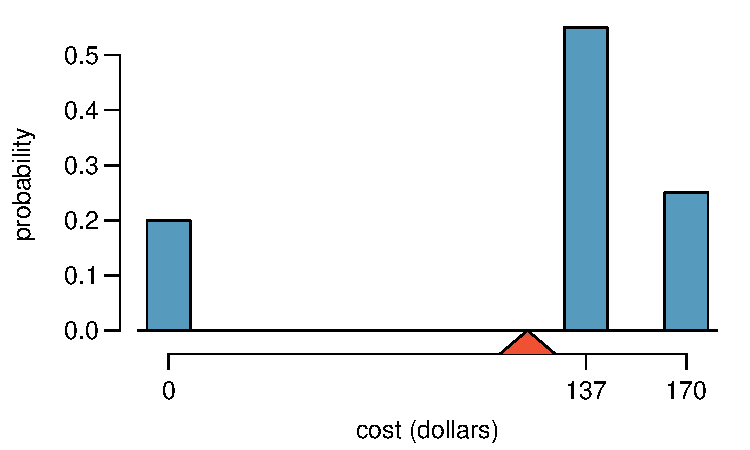
\includegraphics[width=0.72\textwidth]{ch_probability/figures/bookCostDist/bookCostDist}
\caption{Probability distribution for the bookstore's revenue from one student.   The triangle represents the average revenue per student.}
\label{bookCostDist}
\end{figure}

\begin{examplewrap}
\begin{nexample}{What is the average revenue per student for this course?}\label{revFromStudent}
The expected total revenue is \$11,785, and there are 100 students. Therefore the expected revenue per student is $\$11,785/100 =  \$117.85$.
\end{nexample}
\end{examplewrap}


%%
\subsection{Probability distributions}

A \term{probability distribution} is a table of all disjoint outcomes and their associated probabilities. Figure~\ref{diceProb} shows the probability distribution for the sum of two dice.

\begin{onebox}{Rules for probability distributions}
A probability distribution is a list of the possible outcomes with corresponding probabilities that satisfies three rules: \vspace{-2mm}
\begin{enumerate}
\setlength{\itemsep}{0mm}
\item The outcomes listed must be disjoint.
\item Each probability must be between 0 and 1.
\item The probabilities must total 1. \vspace{1mm}
\end{enumerate}\end{onebox}

\begin{exercisewrap}
\begin{nexercise}\label{usHouseholdIncomeDistsExercise}
Figure~\ref{usHouseholdIncomeDists} suggests three distributions for household income in the United States. Only one is correct. Which one must it be? What is wrong with the other two?\footnotemark
\end{nexercise}
\end{exercisewrap}
\footnotetext{The probabilities of (a) do not sum to 1. The second probability in (b) is negative. This leaves (c), which sure enough satisfies the requirements of a distribution. One of the three was said to be the actual distribution of US household incomes, so it must be (c).}

\begin{figure}[hhh]
\centering
\begin{tabular}{l ccc ccc ccc cc}
  \hline
  \ \vspace{-3mm} \\
Dice sum\vspace{0.3mm} & 2 & 3 & 4 & 5 & 6 & 7 & 8 & 9 & 10 & 11 & 12  \\
Probability & $\frac{1}{36}$ & $\frac{2}{36}$ & $\frac{3}{36}$ & $\frac{4}{36}$ & $\frac{5}{36}$ & $\frac{6}{36}$ & $\frac{5}{36}$ & $\frac{4}{36}$ & $\frac{3}{36}$ & $\frac{2}{36}$ & $\frac{1}{36}$\vspace{1mm} \\
   \hline
\end{tabular}
\caption{Probability distribution for the sum of two dice.}
\label{diceProb}
\ \\[5mm]
\begin{tabular}{r | rr rr}
  \hline
Income range (\$1000s) & 0-25    & 25-50    & 50-100     & 100+    \\
  \hline
(a)\hspace{0.2mm}	 & 0.18 & 0.39 & 0.33 & 0.16 \\
(b)				 & 0.38 & -0.27 & 0.52 & 0.37 \\
(c)\hspace{0.2mm}	 & 0.28 & 0.27 & 0.29 & 0.16 \\
  \hline
\end{tabular}
\caption{Proposed distributions of US household incomes (Guided Practice~\ref{usHouseholdIncomeDistsExercise}).}
\label{usHouseholdIncomeDists}
\end{figure}


Chapter~\ref{summarizingData} emphasized the importance of plotting data to provide quick summaries. Probability distributions can also be summarized in a histogram or bar plot. The probability distribution for the sum of two dice is shown in Figure~\ref{diceProb} and its histogram is plotted in Figure~\ref{diceSumDist}. The distribution of US household incomes is shown in Figure~\ref{usHouseholdIncomeDistBar} as a bar plot. The presence of the 100+ category makes it difficult to represent it with a regular histogram.\footnote{It is also possible to construct a distribution plot when income is not artificially binned into four groups. Density histograms for \emph{continuous} distributions are considered in Section~\ref{contDist}.}

\begin{figure}[h]
\centering
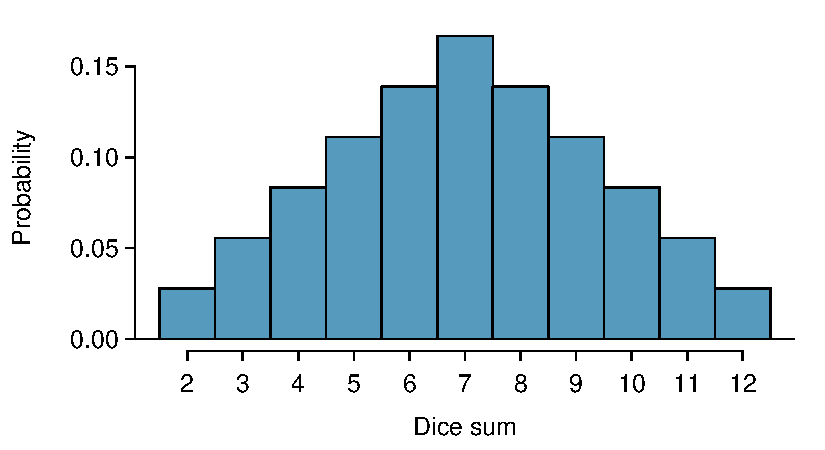
\includegraphics[width=0.65\textwidth]{ch_probability/figures/diceSumDist/diceSumDist}
\caption{A histogram for the probability distribution of the sum of two~dice.}
\label{diceSumDist}
\end{figure}

\begin{figure}[h]
\centering
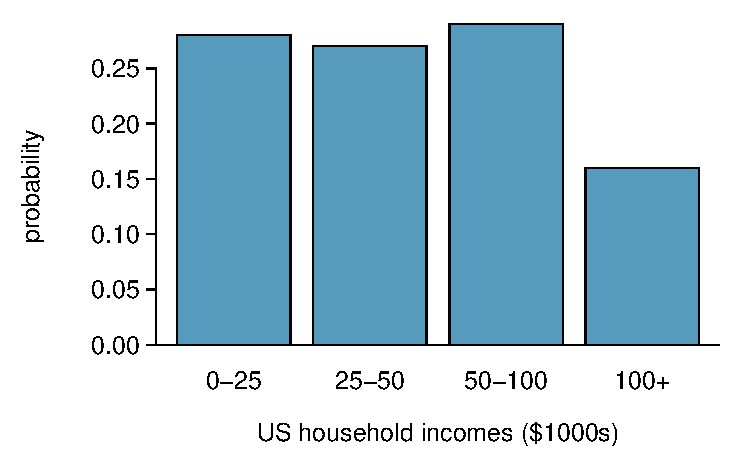
\includegraphics[width=0.63\textwidth]{ch_probability/figures/usHouseholdIncomeDistBar/usHouseholdIncomeDistBar}
\caption{A bar graph for the probability distribution of US household income. Because it is artificially separated into four unequal bins, this graph fails to show the shape or skew of the distribution.}
\label{usHouseholdIncomeDistBar}
\end{figure}

In these bar plots, the bar heights represent the probabilities of outcomes. If the outcomes are numerical and discrete, it is usually (visually) convenient to make a histogram, as in the case of the sum of two dice. Another example of plotting the bars at their respective locations is shown in Figure~\ref{bookCostDist}.



\D{\newpage}

%%
\subsection{Expectation}

\index{expectation|(}

We call a variable or process with a numerical outcome a \term{random variable}, and we usually represent this random variable with a capital letter such as $X$, $Y$, or $Z$. The amount of money a single student will spend on her statistics books is a random variable, and we represent it by $X$.

\begin{onebox}{Random variable}
A random process or variable with a numerical outcome.\end{onebox}

The possible outcomes of $X$ are labeled with a corresponding lower case letter $x$ and subscripts. For example, we write $x_1=\$0$, $x_2=\$137$, and $x_3=\$170$, which occur with probabilities $0.20$, $0.55$, and $0.25$. The distribution of $X$ is summarized in Figure~\ref{bookCostDist} and Figure~\ref{statSpendDist}.

\begin{figure}[hhh]
\centering
\begin{tabular}{l ccc r}
\hline
$i$	  & 1 & 2 & 3  & Total\\
\hline
$x_i$ & \$0 & \$137 & \$170 & --\\
$P(x_i)$ & 0.20 & 0.55 & 0.25 & 1.00 \\
\hline
\end{tabular}
\caption{The probability distribution for the random variable $X$, representing the bookstore's revenue from a single student. We use $P(x_i)$ to represent the probability of $x_i$.}
\label{statSpendDist}
\end{figure}

We computed the average outcome of $X$ as \$117.85 in Example~\ref{revFromStudent}. We call this average the \term{expected value} of $X$, denoted by $E(X)$\index{EX@$E(X)$}. The expected value of a random variable is computed by adding each outcome weighted by its probability:
\begin{align*}
E(X) &= 0 \cdot  P(0) + 137 \cdot  P(137) + 170 \cdot  P(170) \\
	&= 0 \cdot  0.20 + 137 \cdot  0.55 + 170 \cdot  0.25 = 117.85
\end{align*}

\begin{onebox}{Expected value of a discrete random variable}
If $X$ takes outcomes $x_1$, $x_2$, ..., $x_n$ with probabilities $P(x_1)$, $P(x_2)$, ..., $P(x_n)$, the mean, or expected value, of $X$ is the sum of each outcome multiplied by its corresponding probability:
\begin{align*}
\mu_{\scriptscriptstyle{X}} = E(X) &= x_1\cdot P(x_1) + x_2\cdot P(x_2) + \cdots + x_n\cdot P(x_n) \notag \\
	&= \sum_{i=1}^{n}x_i\cdot P(x_i)
\end{align*}
\end{onebox}

The expected value for a random variable represents the average outcome. For example, $E(X)=117.85$ represents the average amount the bookstore expects to make from a single student, which we could also write as $\mu=117.85$. While the bookstore will make more than this on some students and less than this on other students, the average of many randomly selected students will be near \$117.85.

It is also possible to compute the expected value of a continuous random variable (see Section~\ref{contDist}). However, it requires a little calculus and we save it for a later class.\footnote{$\mu_{\scriptscriptstyle{X}} = \int xf(x)dx$ where $f(x)$ represents a function for the density curve.}

In physics, the expectation holds the same meaning as the center of gravity. The distribution can be represented by a series of weights at each outcome, and the mean represents the balancing point. This is represented in Figures~\ref{bookCostDist} and~\ref{bookWts}. The idea of a center of gravity also expands to continuous probability distributions. Figure~\ref{contBalance} shows a continuous probability distribution balanced atop a wedge placed at the mean.

\begin{figure}[h]
\centering
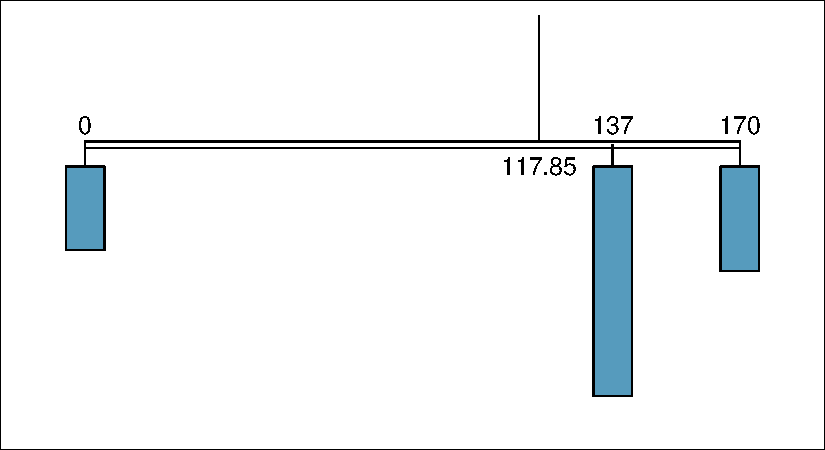
\includegraphics[width=0.72\textwidth]{ch_probability/figures/bookWts/bookWts}
\caption{A weight system representing the probability distribution for $X$. The string holds the distribution at the mean to keep the system balanced.}
\label{bookWts}
\end{figure}

\begin{figure}[h]
\centering
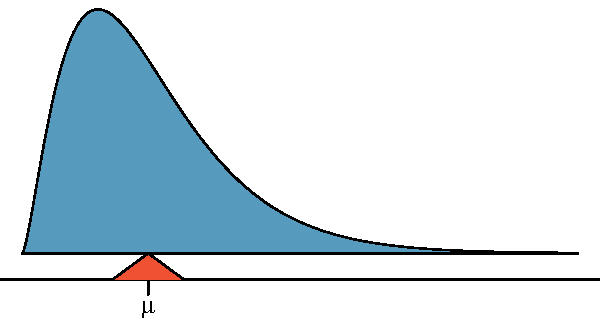
\includegraphics[width=0.7\textwidth]{ch_probability/figures/contBalance/contBalance}
\caption{A continuous distribution can also be balanced at its mean.}
\label{contBalance}
\end{figure}

\index{expectation|)}



\D{\newpage}

%%
\subsection{Variability in random variables}

Suppose you ran the university bookstore. Besides how much revenue you expect to generate, you might also want to know the volatility (variability) in your revenue.

The \indexthis{variance}{variance} and \indexthis{standard deviation}{standard deviation} can be used to describe the variability of a random variable. Section~\ref{variability}
introduced a method for finding the variance and standard deviation for a data set. We first computed deviations from the mean ($x_i - \mu$), squared those deviations, and took an average to get the variance. In the case of a random variable, we again compute squared deviations. However, we take their sum weighted by their corresponding probabilities, just like we did for the expectation. This weighted sum of squared deviations equals the variance, and we calculate the standard deviation by taking the square root of the variance, just as we did in Section~\ref{variability}.

\begin{onebox}{Variance and standard deviation of a discrete random variable}
If $X$ takes outcomes $x_1$, $x_2$, ..., $x_n$ with probabilities $P(x_1)$,  $P(x_2)$, ..., $P(x_n)$ and expected value $\mu_{\scriptscriptstyle{X}}=E(X)$, then to find the standard deviation of $X$, we first find the variance and then take its square root.
\begin{align*}
Var(X) = \sigma^2_x &= (x_1-\mu_{\scriptscriptstyle{X}})^2\cdot P(x_1) + (x_2-\mu_{\scriptscriptstyle{X}})^2\cdot P(x_2) + \cdots +  (x_n-\mu_{\scriptscriptstyle{X}})^2\cdot P(x_n) \notag \\
	&= \sum_{i=1}^{n} (x_i - \mu_{\scriptscriptstyle{X}})^2 \cdot P(x_i) \notag \\
SD(X) = \sigma_{\scriptscriptstyle{X}} &= \sqrt{ \sum_{i=1}^{n} (x_i - \mu_{\scriptscriptstyle{X}})^2 \cdot P(x_i)}
\end{align*}
\end{onebox}

Just as it is possible to compute the mean of a continuous random variable using calculus, we can also use calculus to compute the variance.\footnote{$\sigma^2_x = \int (x - \mu_{\scriptscriptstyle{X}})^2f(x)dx$ where $f(x)$ represents a function for the density curve.} However, this topic is beyond the scope of the AP exam.

\begin{examplewrap}
\begin{nexample}{Compute the expected value, variance, and standard deviation of $X$, the revenue of a single statistics student for the bookstore.}
It is useful to construct a table that holds computations for each outcome separately, then add up the results.
\begin{center}
\begin{tabular}{l rrr r}
\hline
$i$ & 1 & 2&  3& Total \\
\hline
$x_i$ & \$0 & \$137 & \$170 &  \\
$P(x_i)$ & 0.20 & 0.55 & 0.25 &  \\
\hline
$x_i \cdot  P(x_i)$ & 0 & 75.35 & 42.50 & 117.85 \\
\hline
\end{tabular}
\end{center}

Thus, the expected value is $\mu_{\scriptscriptstyle{X}}=117.85$, which we computed earlier. The variance can be constructed using a similar table:
\begin{center}
\begin{tabular}{l rrr r}
\hline
$i$ & 1 & 2 & 3 & Total \\
\hline
$x_i$ & \$0 & \$137 & \$170 &  \\
$P(x_i)$ & 0.20 & 0.55 & 0.25 &  \\
\hline
$x_i - \mu_{\mbox{\tiny\itshape X}}$ & -117.85 & 19.15 & 52.15 &  \\
$(x_i-\mu_{\mbox{\tiny\itshape X}})^2$ & 13888.62 &  366.72 & 2719.62 &  \\
$(x_i-\mu_{\mbox{\tiny\itshape X}})^2\cdot P(x_i)$ & 2777.7 & 201.7 & 679.9 & 3659.3 \\
\hline
\end{tabular}
\end{center}
The variance of $X$ is $\sigma_{\scriptscriptstyle{X}}^2 = 3659.3$, which means the standard deviation is $\sigma_{\scriptscriptstyle{X}} = \sqrt{3659.3} = \$60.49$.
\end{nexample}
\end{examplewrap}

\begin{exercisewrap}
\begin{nexercise}
The bookstore also offers a chemistry textbook for \$159 and a book supplement for \$41. From past experience, they know about 25\% of chemistry students just buy the textbook while 60\% buy both the textbook and supplement.\footnotemark
\begin{enumerate}
\item[(a)] What proportion of students don't buy either book? Assume no students buy the supplement without the textbook.
\item[(b)] Let $Y$ represent the revenue from a single student. Write out the probability distribution of $Y$, i.e. a table for each outcome and its associated probability.
\item[(c)] Compute the expected revenue from a single chemistry student.
\item[(d)] Find the standard deviation to describe the variability associated with the revenue from a single student.
\end{enumerate}
\end{nexercise}
\end{exercisewrap}
\footnotetext{(a) 100\% - 25\% - 60\% = 15\% of students do not buy any books for the class. Part~(b) is represented by the first two lines in the table below. The expectation for part~(c) is given as the total on the line $y_i\cdot P(y_i)$. The result of part~(d) is the square-root of the variance listed on in the total on the last line: $\sigma_{\mbox{\tiny\itshape Y}} = \sqrt{Var(Y)} =\sqrt{4800} =69.28$.
\begin{center}
\begin{tabular}{rrrrr}
$i$ (scenario) & 1 (\resp{noBook}) & 2 (\resp{textbook}) & 3 (\resp{both}) & Total \\
  \hline
$y_i$ & 0.00 & 159.00 & 200.00 &  \\
$P(y_i)$ & 0.15 & 0.25 & 0.60 & \\
\hline
$y_i\cdot P(y_i)$ & 0.00 & 39.75 & 120.00 & $E(Y) = 159.75$\\
$y_i-\mu_{\mbox{\tiny\itshape Y}}$ & -159.75 & -0.75 & 40.25 & \\
$(y_i-\mu_{\mbox{\tiny\itshape Y}})^2$ & 25520.06 & 0.56 & 1620.06 & \\
$(y_i-\mu_{\mbox{\tiny\itshape Y}})^2\cdot P(y_i)$ & 3828.0 & 0.1 & 972.0 & $Var(Y) \approx 4800$ \\
\hline
\end{tabular}
\end{center}}

%%
\subsection{Linear transformations of a random variable}

An online store is selling a limited edition t-shirt.  The maximum a person is allowed to buy is~3.  Let X be a random variable that represents how many of the t-shirts a t-shirt buyer orders.  The probability distribution of X is given in the following table.

\begin{center}
\begin{tabular}{l rrr}
\hline
$x_i$ & 1 & 2 & 3  \\
\hline
$P(x_i)$  & 0.6 & 0.3 & 0.1 \\
\hline
\end{tabular}
\end{center}

Using the methods of the previous section we can find that the mean $\mu_{\scriptscriptstyle{X}} = 1.5$ and the standard deviation $\sigma_{\scriptscriptstyle{X}} = 0.67$.
Suppose that the cost of each t-shirt is \$30 and that there is flat rate \$5 shipping fee.  The amount of money a t-shirt buyer pays, then, is $30X + 5$, where X is the number of t-shirts ordered. To calculate the mean and standard deviation for the amount of money a t-shirt buyers pays, we could define a new variable $Y$ as follows:

\begin{align*}
Y = 30X + 5
\end{align*}

\begin{exercisewrap}
\begin{nexercise}Verify that the distribution of $Y$ is given by the table below.\footnotemark

\begin{center}
\begin{tabular}{l rrr}
\hline
$y_i$ & \$35 & \$65 & \$95  \\
\hline
$P(y_i)$ & 0.6 & 0.3 & 0.1 \\
\hline
\end{tabular}
\end{center}

\end{nexercise}
\end{exercisewrap}
\footnotetext{$30 \times 1 + 5 = 35$;  $30 \times 2 + 5 = 65$; $30 \times 3 + 5 = 95$}

\D{\newpage}

Using this new table, we can compute the mean and standard deviation of the cost for t-shirt orders. However, because Y is a linear transformation of X, we can use the properties from Section~\ref{linearTransformationOfData}. Recall that multiplying every X by 30 multiplies both the mean and standard deviation by 30. Adding 5 only adds 5 to the mean, not the standard deviation. Therefore,
\begin{align*}
\mu_{30X+5}&=E(30X+5) 
	& \sigma_{30X+5}&=SD(30X+5)\\
&= 30\times E(X) + 5
	& &= 30\times SD(X) \\
&= 30\times 1.5+5
	& &= 30 \times 0.67 \\
&= 45.00
	& &= 20.10
\end{align*}
Among t-shirt buyers, they spend an average of \$45.00, with a standard deviation of \$20.10.

\begin{onebox}{Linear transformations of a random variable}
If $X$ is a random variable, then a linear transformation is given by $aX + b$, where $a$ and $b$ are some fixed numbers.
\begin{align*}
E(aX+b) &= a\times E(X) + b
&
SD(aX+b) &= \lvert a\rvert \times SD(X)
\end{align*}
\end{onebox}

%%
\subsection{Linear combinations of random variables}

So far, we have thought of each variable as being a complete story in and of itself. Sometimes it is more appropriate to use a combination of variables. For instance, the amount of time a person spends commuting to work each week can be broken down into several daily commutes. Similarly, the total gain or loss in a stock portfolio is the sum of the gains and losses in its components.

\begin{examplewrap}
\begin{nexample}{John travels to work five days a week. We will use $X_1$ to represent his travel time on Monday, $X_2$ to represent his travel time on Tuesday, and so on. Write an equation using $X_1$, ..., $X_5$ that represents his travel time for the week, denoted by $W$.}
His total weekly travel time is the sum of the five daily values:
$$ W = X_1 + X_2 + X_3 + X_4 + X_5 $$
Breaking the weekly travel time $W$ into pieces provides a framework for understanding each source of randomness and is useful for modeling $W$.
\end{nexample}
\end{examplewrap}

\begin{examplewrap}
\begin{nexample}{It takes John an average of 18 minutes each day to commute to work. What would you expect his average commute time to be for the week?}
We were told that the average (i.e. expected value) of the commute time is 18 minutes per day: $E(X_i) = 18$. To get the expected time for the sum of the five days, we can add up the expected time for each individual day:
\begin{align*}
E(W) &= E(X_1 + X_2 + X_3 + X_4 + X_5) \\
	&= E(X_1) + E(X_2) + E(X_3) + E(X_4) + E(X_5) \\
	&= 18 + 18 + 18 + 18 + 18 = 90\text{ minutes}
\end{align*}
The expectation of the total time is equal to the sum of the expected individual times. More generally, the expectation of a sum of random variables is always the sum of the expectation for each random variable.
\end{nexample}
\end{examplewrap}

\begin{exercisewrap}
\begin{nexercise} \label{elenaIsSellingATVAndBuyingAToasterOvenAtAnAuction}
Elena is selling a TV at a cash auction and also intends to buy a toaster oven in the auction. If $X$ represents the profit for selling the TV and $Y$ represents the cost of the toaster oven, write an equation that represents the net change in Elena's cash.\footnotemark
\end{nexercise}
\end{exercisewrap}
\footnotetext{She will make $X$ dollars on the TV but spend $Y$ dollars on the toaster oven: $X-Y$.}

\begin{exercisewrap}
\begin{nexercise}
Based on past auctions, Elena figures she should expect to make about \$175 on the TV and pay about \$23 for the toaster oven. In total, how much should she expect to make or spend?\footnotemark
\end{nexercise}
\end{exercisewrap}
\footnotetext{$E(X-Y) = E(X) - E(Y) = 175 - 23 = \$152$. She should expect to make about \$152.}

\begin{exercisewrap}
\begin{nexercise} \label{explainWhyThereIsUncertaintyInTheSum}
Would you be surprised if John's weekly commute wasn't exactly 90 minutes or if Elena didn't make exactly \$152? Explain.\footnotemark
\end{nexercise}
\end{exercisewrap}
\footnotetext{No, since there is probably some variability. For example, the traffic will vary from one day to next, and auction prices will vary depending on the quality of the merchandise and the interest of the attendees.}

Two important concepts concerning combinations of random variables have so far been introduced. First, a final value can sometimes be described as the sum of its parts in an equation. Second, intuition suggests that putting the individual average values into this equation gives the average value we would expect in total. This second point needs clarification -- it is guaranteed to be true in what are called \emph{linear combinations of random variables}.

A \term{linear combination} of two random variables $X$ and $Y$ is a fancy phrase to describe a combination
$$ aX + bY$$
where $a$ and $b$ are some fixed and known numbers. For John's commute time, there were five random variables -- one for each work day -- and each random variable could be written as having a fixed coefficient of 1:
$$ 1X_1 + 1 X_2 + 1 X_3 + 1 X_4 + 1 X_5 $$
For Elena's net gain or loss, the $X$ random variable had a coefficient of +1 and the $Y$ random variable had a coefficient of -1.

When considering the average of a linear combination of random variables, it is safe to plug in the mean of each random variable and then compute the final result. For a few examples of nonlinear combinations of random variables -- cases where we cannot simply plug in the means -- see the footnote.\footnote{If $X$ and $Y$ are random variables, consider the following combinations: $X^{1+Y}$, $X\times Y$, $X/Y$. In such cases, plugging in the average value for each random variable and computing the result will not generally lead to an accurate average value for the end result.}

\begin{onebox}{Linear combinations of random variables and the average result}
If $X$ and $Y$ are random variables, then a linear combination of the random variables is given by $aX + bY$, where $a$ and $b$ are some fixed numbers. To compute the average value of a linear combination of random variables, plug in the average of each individual random variable and compute the result:
\begin{align*}
E(aX+bY) = a\times E(X) + b\times E(Y)
\end{align*}
Recall that the expected value is the same as the mean, i.e. $E(X) = \mu_{\mbox{\tiny\itshape X}}$.
\end{onebox}

\D{\newpage}

\begin{examplewrap}
\begin{nexample}{Leonard has invested \$6000 in Google Inc. (stock ticker: GOOG) and \$2000 in Exxon Mobil Corp. (XOM). If $X$ represents the change in Google's stock next month and $Y$ represents the change in Exxon Mobil stock next month, write an equation that describes how much money will be made or lost in Leonard's stocks for the month.}
For simplicity, we will suppose $X$ and $Y$ are not in percents but are in decimal form (e.g. if Google's stock increases 1\%, then $X=0.01$; or if it loses 1\%, then $X=-0.01$). Then we can write an equation for Leonard's gain as
\begin{align*}
\$6000\times X + \$2000\times Y
\end{align*}
If we plug in the change in the stock value for $X$ and $Y$, this equation gives the change in value of Leonard's stock portfolio for the month. A positive value represents a gain, and a negative value represents a loss.
\end{nexample}
\end{examplewrap}

\begin{exercisewrap}
\begin{nexercise}\label{expectedChangeInLeonardsStockPortfolio}
Suppose Google and Exxon Mobil stocks have recently been rising 2.1\% and 0.4\% per month, respectively. Compute the expected change in Leonard's stock portfolio for next month.\footnotemark
% library(stockPortfolio); gr <- getReturns(c("GOOG", "XOM"), start="2006-01-01"); gr
\end{nexercise}
\end{exercisewrap}
\footnotetext{$E(\$6000\times X + \$2000\times Y) = \$6000\times 0.021 + \$2000\times 0.004 = \$134$.}

\begin{exercisewrap}
\begin{nexercise}
You should have found that Leonard expects a positive gain in Guided Practice~\ref{expectedChangeInLeonardsStockPortfolio}. However, would you be surprised if he actually had a loss this month?\footnotemark
\end{nexercise}
\end{exercisewrap}
\footnotetext{No. While stocks tend to rise over time, they are often volatile in the short term.}

%%
\subsection{Variability in linear combinations of random variables}

Quantifying the average outcome from a linear combination of random variables is helpful, but it is also important to have some sense of the uncertainty associated with the total outcome of that combination of random variables. The expected net gain or loss of Leonard's stock portfolio was considered in Guided Practice~\ref{expectedChangeInLeonardsStockPortfolio}. However, there was no quantitative discussion of the volatility of this portfolio. For instance, while the average monthly gain might be about \$134 according to the data, that gain is not guaranteed. Figure~\ref{changeInLeonardsStockPortfolioFor36Months} shows the monthly changes in a portfolio like Leonard's during the 36 months from 2009 to 2011. The gains and losses vary widely, and quantifying these fluctuations is important when investing in stocks.

\begin{figure}[ht]
\centering
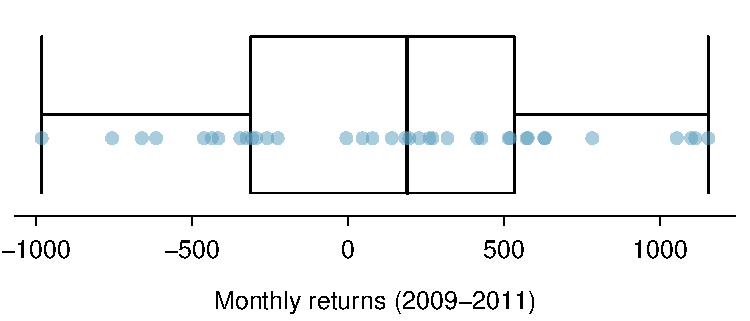
\includegraphics[width=0.55\textwidth]{ch_probability/figures/changeInLeonardsStockPortfolioFor36Months/changeInLeonardsStockPortfolioFor36Months}
\caption{The change in a portfolio like Leonard's for the 36 months from 2009 to 2011, where \$6000 is in Google's stock and \$2000 is in Exxon Mobil's.}
\label{changeInLeonardsStockPortfolioFor36Months}
\end{figure}

Just as we have done in many previous cases, we use the variance and standard deviation to describe the uncertainty associated with Leonard's monthly returns. To do so, the standard deviations and variances of each stock's monthly return will be useful, and these are shown in Figure~\ref{sumStatOfGOOGXOM}. The stocks' returns are nearly independent.

\begin{figure}
\centering
\begin{tabular}{lrrr}
\hline
	& Mean ($\bar{x}$) & Standard deviation ($s$) & Variance ($s^2$) \\
\hline
GOOG & 0.0210	& 0.0849				&	0.0072	\\
XOM & 0.0038		& 0.0520					&	0.0027	\\
\hline
\end{tabular}
\caption{The mean, standard deviation, and variance of the GOOG and XOM stocks. These statistics were estimated from historical stock data, so notation used for sample statistics has been used.}
\label{sumStatOfGOOGXOM}
\end{figure}

We want to describe the uncertainty of Leonard's monthly returns by finding the standard deviation of the return on his combined portfolio. First, we note that the variance of a sum has a nice property: the variance of a sum is the sum of the variances. That~is, if X and Y are independent random variables:
\begin{align*}
Var(X + Y) &= Var(X) + Var(Y)
\end{align*}
Because the standard deviation is the square root of the variance, we can rewrite this equation using standard deviations:
\begin{align*}
(SD_{X + Y})^2 = (SD_X)^2 + (SD_Y)^2
\end{align*}
This equation might remind you of a theorem from geometry:  $c^2 = a^2 + b^2$. The equation for the standard deviation of the sum of two independent random variables looks analogous to the Pythagorean Theorem. Just as the Pythagorean Theorem only holds for right triangles, this equation only holds when X and Y are \emph{independent}.\footnote{Another word for independent is orthogonal, meaning right angle!  When X and Y are dependent, the equation for $SD_{X+Y}$ becomes analogous to the law of cosines.}

\begin{onebox}{Standard deviation of the sum and difference of random variables}
If X and Y are \emph{independent} random variables:
\begin{align*}
SD_{X + Y} = SD_{X - Y} = \sqrt{(SD_X)^2 + (SD_Y)^2}
\end{align*}
\end{onebox}

Because $SD_Y$ = $SD_{-Y}$, the standard deviation of the difference of two variables equals the standard deviation of the sum of two variables. This property holds for more than two variables as well. For example, if X, Y, and Z are independent random variables:
\begin{align*}
SD_{X + Y + Z} = SD_{X - Y - Z}  = \sqrt{(SD_X)^2 + (SD_Y)^2 + (SD_Z)^2}
\end{align*}

If we need the standard deviation of a linear combination of independent variables, such as $aX + bY$, we can consider $aX$ and $bY$ as two new variables. Recall that multiplying all of the values of variable by a positive constant multiplies the standard deviation by that constant. Thus, $SD_{aX}$ =  $a \times SD_X$ and $SD_{bY}$ =  $b \times SD_Y$. It follows that:
\begin{align*}
SD_{aX + bY} = \sqrt{(a \times SD_X)^2 + (b \times SD_Y)^2}
\end{align*}
This equation can be used to compute the standard deviation of Leonard's monthly return. Recall that Leonard has \$6,000 in Google stock and \$2,000 in Exxon Mobil's stock. From Figure~\ref{sumStatOfGOOGXOM}, the standard deviation of Google stock is 0.0849 and the standard deviation of Exxon Mobile stock is 0.0520.
\begin{align*}
SD_{6000X + 2000Y}
	&= \sqrt{(6000\times SD_X)^2 + (2000\times SD_Y)^2} \\
	&= \sqrt{(6000\times 0.0849)^2 + (2000\times .0520)^2} \\
	&= \sqrt{\text{270,304}} = 520
\end{align*}
The standard deviation of the total is \$520. While an average monthly return of \$134 on an \$8000 investment is nothing to scoff at, the monthly returns are so volatile that Leonard should not expect this income to be very stable.

\begin{onebox}{Standard deviation of linear combinations of random variables}
To find the standard deviation of a linear combination of random variables, we first consider $aX$ and $bY$ separately. We find the standard deviation of each, and then we apply the equation for the standard deviation of the sum of two variables:
\begin{align*}
SD_{aX + bY} = \sqrt{(a\times SD_X)^2 + (b\times SD_Y)^2}
\end{align*}
This equation is valid as long as the random variables $X$ and $Y$ are \emph{independent} of each other.\end{onebox}

\begin{examplewrap}
\begin{nexample}{Suppose John's daily commute has a standard deviation of 4 minutes. What is the uncertainty in his total commute time for the week?} \label{sdOfJohnsCommuteWeeklyTime}
The expression for John's commute time is
\begin{align*}
X_1 + X_2 + X_3 + X_4 + X_5
\end{align*}
Each coefficient is 1, so the standard deviation of the total weekly commute time is
\begin{align*}
\text{SD}&= \sqrt{(1 \times 4)^2 + (1 \times 4)^2 + (1 \times 4)^2 + (1 \times 4)^2 + (1 \times 4)^2} \\
&= \sqrt{5\times (4)^2} \\
&= 8.94
\end{align*}
The standard deviation for John's weekly work commute time is about 9 minutes.
\end{nexample}
\end{examplewrap}

\begin{exercisewrap}
\begin{nexercise}
The computation in Example~\ref{sdOfJohnsCommuteWeeklyTime} relied on an important assumption: the commute time for each day is independent of the time on other days of that week. Do you think this is valid? Explain.\footnotemark
\end{nexercise}
\end{exercisewrap}
\footnotetext{One concern is whether traffic patterns tend to have a weekly cycle (e.g. Fridays may be worse than other days). If that is the case, and John drives, then the assumption is probably not reasonable. However, if John walks to work, then his commute is probably not affected by any weekly traffic cycle.}

\begin{exercisewrap}
\begin{nexercise}\label{elenaIsSellingATVAndBuyingAToasterOvenAtAnAuctionVariability}
Consider Elena's two auctions from Guided Practice~\ref{elenaIsSellingATVAndBuyingAToasterOvenAtAnAuction} on page~\pageref{elenaIsSellingATVAndBuyingAToasterOvenAtAnAuction}. Suppose these auctions are approximately independent and the variability in auction prices associated with the TV and toaster oven can be described using standard deviations of \$25 and \$8. Compute the standard deviation of Elena's net gain.\footnotemark
\end{nexercise}
\end{exercisewrap}
\footnotetext{The equation for Elena can be written as:  $(1)\times X + (-1)\times Y$.
To find the SD of this new variable we do:
\begin{align*}
SD_{(1)\times X + (-1)\times Y} = \sqrt{(1\times SD_X)^2 + (-1\times SD_Y)^2 = (1\times 25)^2 + (-1\times 8)^2} = 26.25
\end{align*}
The SD is about \$26.25.}

Consider again Guided Practice~\ref{elenaIsSellingATVAndBuyingAToasterOvenAtAnAuctionVariability}. The negative coefficient for $Y$ in the linear combination was eliminated when we squared the coefficients. This generally holds true: negatives in a linear combination will have no impact on the variability computed for a linear combination, but they do impact the expected value computations.

\index{random variable|)}

\D{\newpage}

%%
\subsection*{Section summary}

\begin{itemize}

\item A \term{discrete probability distribution} can be summarized in a table that consists of all possible outcomes of a random variable and the probabilities of those outcomes.  The outcomes must be disjoint, and the sum of the probabilities must equal 1.

\item A probability distribution can be represented with a histogram and, like the distributions of data that we saw in Chapter 2, can be summarized by its \term{center}, \term{spread}, and \term{shape}.

\item When given a probability distribution table, we can calculate the \term{mean} (expected value) and \term{standard deviation} of a random variable using the following formulas.  \vspace{-1mm}
\begin{flalign*}
E(X) = \mu_{\scriptscriptstyle{X}} &= \sum{x_i\cdot P(x_i)} &\\
&= x_1\cdot P(x_1) + x_2\cdot P(x_2) + \cdots + x_n\cdot P(x_n) \notag \\
Var(X) = \sigma^2_x &= \sum(x_i - \mu_{\scriptscriptstyle{X}})^2 \cdot P(x_i) \\
	SD(X) = \sigma_{\scriptscriptstyle{X}} 
	&=\sqrt{\sum(x_i - \mu_{\scriptscriptstyle{X}})^2 \cdot P(x_i)} \notag \\
	 &=\sqrt{(x_1-\mu_{\scriptscriptstyle{X}})^2\cdot P(x_1) + (x_2-\mu_{\scriptscriptstyle{X}})^2\cdot P(x_2) + \cdots +  (x_n-\mu_{\scriptscriptstyle{X}})^2\cdot P(x_n) }
\end{flalign*}
We can think of $P(x_i)$ as the \emph{weight}, and each term is weighted its appropriate amount.

\item The \term{mean} of a probability distribution does not need to be a value in the distribution.  It represents the average of many, many repetitions of a random process.  The \term{standard deviation} represents the typical variation of the outcomes from the mean, when the random process is repeated over and over.

\item \textbf{Linear transformations}.  Adding a constant to every value in a probability distribution adds that value to the mean, but it does not affect the standard deviation.  When multiplying every value by a constant, this multiplies the mean by the constant and it multiplies the standard deviation by the absolute value of the constant.
\item \termsub{Combining random variables}{combining random variables}\index{random variable!combine|textbf}.  Let $X$ and $Y$ be random variables and let $a$ and $b$ be constants.\vspace{-1mm}
\begin{itemize}
 \item The expected value of the sum is the sum of the expected values.

\item[] $E(X+Y) = E(X) + E(Y)$
  
\item[] $E(aX+bY) = a\times E(X) + b\times E(Y)$
\end{itemize}

\begin{itemize}
\item When X and Y are \term{independent}: 
The standard deviation of a sum or a difference is the square root of the sum of each standard deviation squared. 
\item[]
  $SD(X + Y) =  \sqrt{(SD(X))^2 + (SD(Y))^2}$ 

\item[] $SD(X - Y) =  \sqrt{(SD(X))^2 + (SD(Y))^2}$
  
\item[] $SD(aX + bY) = \sqrt{(a\times SD(X))^2 + (b\times SD(Y))^2}$
 
\end{itemize}

The SD properties require that $X$ and $Y$ be independent.  The expected value properties hold true whether or not $X$ and $Y$ are independent.
\end{itemize}



%%%%%%%%%%Section Exercises
{\exercisesheader{}

% 37

\eoce{\qt{College smokers\label{college_smokers}} At a university, 13\% of 
students smoke.
\begin{parts}
\item Calculate the expected number of smokers in a random sample of 100 students 
from this university.
\item The university gym opens at 9 am on Saturday mornings. One Saturday morning 
at 8:55 am there are 27 students outside the gym waiting for it to open. Should 
you use the same approach from part (a) to calculate the expected number of 
smokers among these 27 students?
\end{parts}
}{}

% 38

\eoce{\qt{Ace of clubs wins\label{ace_of_clubs}} Consider the following card game 
with a well-shuffled deck of cards. If you draw a red card, you win nothing. If 
you get a spade, you win \$5. For any club, you win \$10 plus an extra \$20 for 
the ace of clubs.
\begin{parts}
\item Create a probability model for the amount you win at this game. Also, find 
the expected winnings for a single game and the standard deviation of the 
winnings.
\item What is the maximum amount you would be willing to pay to play this game? 
Explain your reasoning.
\end{parts}
}{}

% 39

\eoce{\qt{Hearts win\label{hearts}} In a new card game, you start
with a well-shuffled full deck and draw 3 cards without replacement.
If you draw 3 hearts, 
you win \$50. If you draw 3 black cards, you win \$25. For any other draws, you 
win nothing.
\begin{parts}
\item Create a probability model for the amount you win at this game, and find 
the expected winnings. Also compute the standard deviation of this distribution.
\item If the game costs \$5 to play, what would be the expected value and 
standard deviation of the net profit (or loss)? \textit{(Hint: 
profit = winnings $-$ cost; $X-5$)}
\item If the game costs \$5 to play, should you play this game? Explain.
\end{parts}
}{}

% 40

\eoce{\qtq{Is it worth it\label{worth_it}} Andy is always looking for ways to 
make money fast. Lately, he has been trying to make money by gambling. Here is 
the game he is considering playing: The game costs \$2 to play. He draws a card 
from a deck. If he gets a number card (2-10), he wins nothing. For any face card (
jack, queen or king), he wins \$3. For any ace, he wins \$5, and he wins an 
\textit{extra} \$20 if he draws the ace of clubs.
\begin{parts}
\item Create a probability model and find Andy's expected profit per game.
\item Would you recommend this game to Andy as a good way to make money? Explain.
\end{parts}
}{}

% 41

\eoce{\qt{Portfolio return\label{portfolio_return}} A portfolio's value increases 
by 18\% during a financial boom and by 9\% during normal times. It decreases by 
12\% during a recession. What is the expected return on this portfolio if each 
scenario is equally likely?
}{}

% 42

\eoce{\qt{Baggage fees\label{baggage_fees}} An airline charges the following 
baggage fees: \$25 for the first bag and \$35 for the second. Suppose 54\% of 
passengers have no checked luggage, 34\% have one piece of checked luggage and 
12\% have two pieces. We suppose a negligible portion of people check more than 
two bags.
\begin{parts}
\item Build a probability model, compute the average revenue per passenger, and 
compute the corresponding standard deviation.
\item About how much revenue should the airline expect for a flight of 120 
passengers? With what standard deviation? Note any assumptions you make and if 
you think they are justified.
\end{parts}
}{}

% 43

\eoce{\qt{American roulette\label{roulette_american}} The game of American 
roulette involves spinning a wheel with 38 slots: 18 red, 18 black, and 2 green. 
A ball is spun onto the wheel and will eventually land in a slot, where each slot 
has an equal chance of capturing the ball. Gamblers can place bets on red or 
black. If the ball lands on their color, they double their money. If it lands on 
another color, they lose their money. Suppose you bet \$1 on red. What's the 
expected value and standard deviation of your winnings?
}{}

% 44

\eoce{\qt{European roulette\label{roulette_european}} The game of European 
roulette involves spinning a wheel with 37 slots: 18 red, 18 black, and 1 green. 
A ball is spun onto the wheel and will eventually land in a slot, where each slot 
has an equal chance of capturing the ball. Gamblers can place bets on red or 
black. If the ball lands on their color, they double their money. If it lands on 
another color, they lose their money.
\begin{parts}
\item Suppose you play roulette and bet \$3 on a single round. What is the 
expected value and standard deviation of your total winnings?
\item Suppose you bet \$1 in three different rounds. What is the expected value 
and standard deviation of your total winnings?
\item How do your answers to parts (a) and (b) compare? What does this say about 
the riskiness of the two games?
\end{parts}
}{}
}




%_______________________________________
\section[Continuous distributions]{Continuous distributions }
\label{contDist}

\sectionintro{
\noindent%
So far we have looked only at cases where the random variable takes on integer values.
What happens when we consider random variables that produce a continuous numerical variable, such as wait time for a bus?
In this section, we introduce the concept of a continuous distribution.
In the next chapter, you will encounter the most famous continuous distribution of all.\footnote{It's the normal distribution!}


%%
\subsection*{Learning objectives}
\begin{enumerate}
\setlength{\itemsep}{0mm}
\item Understand the difference between a discrete random variable and a continuous random variable.

\item Recognize that when working with continuous probability distributions area represents probability and the total area under the curve must equal 1. 

\end{enumerate}
}

%%
\subsection{From histograms to continuous distributions}

\index{data!FCID|(}
\index{hollow histogram|(}
\begin{examplewrap}
\begin{nexample}{Figure~\ref{fdicHistograms} shows a few different hollow histograms of the variable \var{height} for 3 million US adults from the mid-90's.\footnotemark\, How does changing the number of bins allow you to make different interpretations of the data?}\label{usHeights}
Adding more bins provides greater detail. This sample is extremely large, which is why much smaller bins still work well. Usually we do not use so many bins with smaller sample sizes since small counts per bin mean the bin heights are very volatile.
\end{nexample}
\end{examplewrap}
\footnotetext{This sample can be considered a simple random sample from the US population. It relies on the USDA Food Commodity Intake Database.} 

\begin{figure}[ht]
\centering
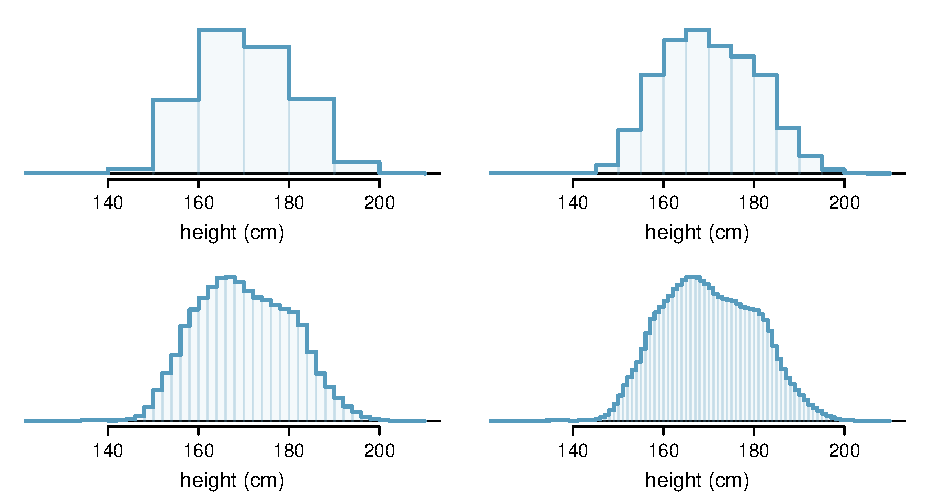
\includegraphics[width=\textwidth]{ch_probability/figures/fdicHistograms/fdicHistograms}
\caption{Four hollow histograms of US adults heights with varying bin widths.}
\label{fdicHistograms}
\end{figure}

\begin{examplewrap}
\begin{nexample}{What proportion of the sample is between 180 cm and 185 cm tall (about 5'11" to 6'1")?}\label{contDistProb}
We can add up the heights of the bins in the range 180 cm and 185 and divide by the sample size. For instance, this can be done with the two shaded bins shown in Figure~\ref{usHeightsHist180185}. The two bins in this region have counts of 195,307 and 156,239 people, resulting in the following estimate of the probability:
\begin{eqnarray*}
\frac{195307+156239}{\text{3,000,000}} = 0.1172
\end{eqnarray*}
This fraction is the same as the proportion of the histogram's area that falls in the range 180 to 185~cm.
\end{nexample}
\end{examplewrap}

\begin{figure}
\centering
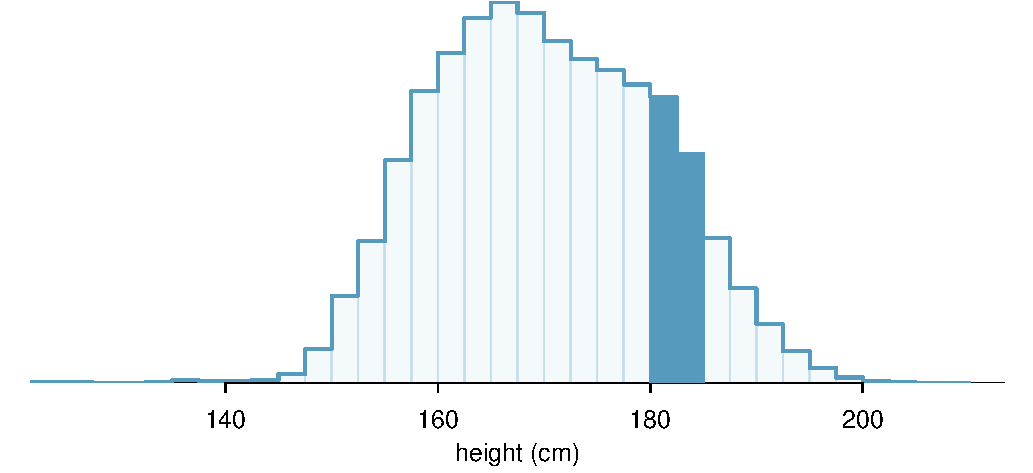
\includegraphics[width=0.95\textwidth]{ch_probability/figures/usHeightsHist180185/usHeightsHist180185}
\caption{A histogram with bin sizes of 2.5 cm. The shaded region represents individuals with heights between 180 and 185 cm.}
\label{usHeightsHist180185}
\end{figure}

\D{\newpage}

Examine the transition from a boxy hollow histogram in the top-left of Figure~\ref{fdicHistograms} to the much smoother plot in the lower-right. In this last plot, the bins are so slim that the hollow histogram is starting to resemble a smooth curve. This suggests the population height as a \emph{continuous} numerical variable might best be explained by a curve that represents the outline of extremely slim bins.

This smooth curve represents a \term{probability density function} (also called a \term{density} or \term{distribution}), and such a curve is shown in Figure~\ref{fdicHeightContDist} overlaid on a histogram of the sample. A density has a special property: the total area under the density's curve is 1.

\begin{figure}[tbh]
\centering
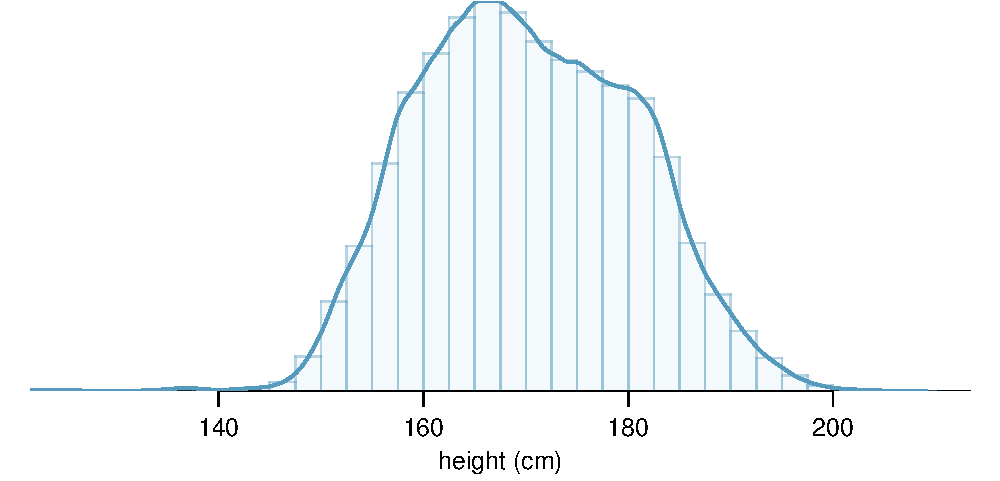
\includegraphics[width=0.87\textwidth]{ch_probability/figures/fdicHeightContDist/fdicHeightContDist}
\caption{The continuous probability distribution of heights for US adults.}
\label{fdicHeightContDist}
\end{figure}

\index{hollow histogram|)}


%%
\subsection{Probabilities from continuous distributions}

We computed the proportion of individuals with heights 180 to 185 cm in Example~\ref{contDistProb} as a fraction:
\begin{eqnarray*}
\frac{\text{number of people between 180 and 185}}{\text{total sample size}}
\end{eqnarray*}
We found the number of people with heights between 180 and 185 cm by determining the fraction of the histogram's area in this region. Similarly, we can use the area in the shaded region under the curve to find a probability (with the help of a computer):
\begin{eqnarray*}
P(\text{\var{height} between 180 and 185})
	= \text{area between 180 and 185}
	= 0.1157
\end{eqnarray*}
The probability that a randomly selected person is between 180 and 185 cm is 0.1157. This is very close to the estimate from Example~\ref{contDistProb}: 0.1172.


\begin{exercisewrap}
\begin{nexercise}
Three US adults are randomly selected. The probability a single adult is between 180 and 185 cm is 0.1157.\footnotemark \vspace{-1.5mm}
\begin{enumerate}
\setlength{\itemsep}{0mm}
\item[(a)] What is the probability that all three are between 180 and 185 cm tall?
\item[(b)] What is the probability that none are between 180 and 185 cm?
\end{enumerate}
\end{nexercise}
\end{exercisewrap}
\footnotetext{Brief answers: (a) $0.1157 \times 0.1157 \times 0.1157 = 0.0015$. (b) $(1-0.1157)^3 = 0.692$}

\D{\newpage}

\begin{examplewrap}
\begin{nexample}{What is the probability that a randomly selected person is \textbf{exactly} 180~cm? Assume you can measure perfectly.}
\label{probabilityOfExactly180cm}
This probability is zero. A person might be close to 180 cm, but not exactly 180 cm tall. This also makes sense with the definition of probability as area; there is no area captured between 180~cm and 180~cm.
\end{nexample}
\end{examplewrap}

\begin{exercisewrap}
\begin{nexercise}
Suppose a person's height is rounded to the nearest centimeter. Is there a chance that a random person's \textbf{measured} height will be 180~cm?\footnotemark
\end{nexercise}
\end{exercisewrap}
\footnotetext{This has positive probability. Anyone between 179.5 cm and 180.5 cm will have a \emph{measured} height of 180 cm. This is probably a more realistic scenario to encounter in practice versus Example~\ref{probabilityOfExactly180cm}.}

\index{data!FCID|)}


\D{\newpage}

%%
\subsection*{Section summary}
\begin{itemize}
\item Histograms use bins with a specific width to display the distribution of a variable.  When there is enough data and the data does not have gaps, as the bin width gets smaller and smaller, the histogram begins to resemble a smooth curve, or a \term{continuous distribution}. 

\item Continuous distributions are often used to approximate relative frequencies and probabilities.  In a continuous distribution, the \emph{area under the curve} corresponds to relative frequency or probability.  The total area under a continuous probability distribution must equal 1.  

\item Because the area under the curve for a single point is zero, the probability of any specific value is zero.  This implies that, for example, $P(X < 5) = P(X \le 5)$ for a continuous probability distribution.

\item Finding areas under curves is challenging; it is common to use distribution tables, calculators, or other technology to find such areas.

\end{itemize}



%%%%%%Section Exercises
{\exercisesheader{}

% 45

\eoce{\qt{Cat weights\label{cat_weights}} The histogram shown below represents 
the weights (in kg) of 47 female and 97 male cats. \footfullcite{cats} \\
\begin{minipage}[c]{0.47\textwidth}
\begin{parts}
\item What fraction of these cats weigh less than 2.5 kg?
\item What fraction of these cats weigh between 2.5 and 2.75 kg?
\item What fraction of these cats weigh between 2.75 and 3.5 kg?
\end{parts} \vspace{27mm}
\end{minipage}
\begin{minipage}[c]{0.05\textwidth}
$\:$ 
\end{minipage}
\begin{minipage}[c]{0.48\textwidth}
\begin{center}
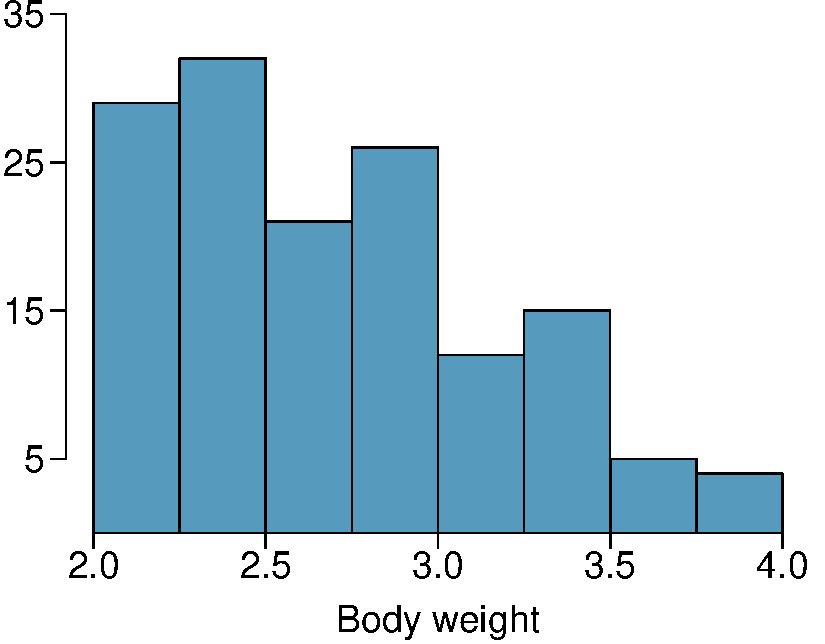
\includegraphics[width=\textwidth]{ch_probability/figures/eoce/cat_weights/cat_weights.pdf}
\end{center}
\end{minipage}
}{}

% 46

\eoce{\qt{Income and gender\label{income_gender}} The relative frequency table 
below displays the distribution of annual total personal income (in 2009 
inflation-adjusted dollars) for a representative sample of 96,420,486 Americans. 
These data come from the American Community Survey for 2005-2009. This sample is 
comprised of 59\% males and 41\% females. \footfullcite{acsIncome2005-2009} \\

\noindent\begin{minipage}[c]{0.60\textwidth}
\begin{parts}
\item Describe the distribution of total personal income.
\item What is the probability that a randomly chosen US resident makes less than 
\$50,000 per year?
\item What is the probability that a randomly chosen US resident makes less than 
\$50,000 per year and is female? Note any assumptions you make.
\item The same data source indicates that 71.8\% of females make less than 
\$50,000 per year. Use this value to determine whether or not the assumption you 
made in part (c) is valid.
\end{parts} 
\end{minipage}
\begin{minipage}[c]{0.4\textwidth}
{\small
\begin{center}
\begin{tabular}{lr}
  \hline
\textit{Income}         & \textit{Total} \\
  \hline
\$1 to \$9,999 or loss  & 2.2\% \\
\$10,000 to \$14,999    & 4.7\% \\
\$15,000 to \$24,999    & 15.8\% \\
\$25,000 to \$34,999    & 18.3\% \\
\$35,000 to \$49,999    & 21.2\% \\
\$50,000 to \$64,999    & 13.9\% \\
\$65,000 to \$74,999    & 5.8\% \\
\$75,000 to \$99,999    & 8.4\% \\
\$100,000 or more       & 9.7\% \\
   \hline
\end{tabular}
\end{center}
}
\end{minipage}
}{}
}


%______________________________________________
\reviewchapterheader{}

\noindent This chapter focused on understanding likelihood and chance variation, first by solving individual probability questions and then by investigating probability distributions. 
\\
\\The main probability techniques covered in this chapter are as follows:
\begin{itemize}
\item The \term{General Multiplication Rule} for \textbf{and} probabilities (intersection), along with the special case when events are \term{independent}.
\item The \term{General Addition Rule} for \textbf{or} probabilities (union), along with the special case when events are \term{mutually exclusive}.  
\item The \term{Conditional Probability Rule}.
\item Tree diagrams and \term{Bayes' Theorem} to solve more complex conditional problems.
\item The \termsub{Binomial Formula}{binomial formula} for finding the probability of exactly $x$ successes in $n$ independent trials.
\item \termsub{Simulations}{simulation} and the use of random digits to estimate probabilities.
\end{itemize}
Fundamental to all of these problems is understanding when events are independent and when they are mutually exclusive.  Two events are \term{independent} when the outcome of one does not affect the outcome of the other, i.e. $P(A | B) = P(A)$.  Two events are \term{mutually exclusive} when they cannot both happen together, i.e. $P(A \text{ and } B) = 0$.
\\ 
\\
Moving from solving individual probability questions to studying probability distributions helps us better understand chance processes and quantify expected chance variation. 
\begin{itemize}
\item For a \term{discrete probability distribution}, the \term{sum} of the probabilities must equal 1.  For a \term{continuous probability distribution}, the \term{area under the curve} represents a probability and the total area under the curve must equal~1.

\item As with any distribution, one can calculate the mean and standard deviation of a probability distribution.  In the context of a probability distribution, the \term{mean} and \term{standard deviation} describe the average and the typical  deviation from the average, respectively, after many, many repetitions of the chance process.  

\item A probability distribution can be summarized by its \term{center} (mean, median), \term{spread} (SD, IQR), and \term{shape} (right skewed, left skewed, approximately symmetric).  

\item Adding a constant to every value in a probability distribution adds that value to the mean, but it does not affect the standard deviation. When multiplying every value by a constant, this multiplies the mean by the constant and it multiplies the standard deviation by the absolute value of the
constant.

\item The mean of the sum of two random variables equals the sum of the means.  However, this is not true for standard deviations.  Instead, when finding the standard deviation of a sum or difference of random variables, take the square root of the sum of each of the standard deviations squared.

\end{itemize}
The study of probability is useful for measuring uncertainty and assessing risk.  In addition, probability serves as the foundation for inference, providing a framework for evaluating when an outcome falls outside of the range of what would be expected by chance alone.

